\documentclass[a4paper]{article}

\usepackage[utf8]{inputenc}
\usepackage[portuges]{babel}
\usepackage{graphicx}
\usepackage{a4wide}
\usepackage[pdftex]{hyperref}
\usepackage{float}
\usepackage{indentfirst}
\usepackage{subcaption}

\begin{document}

\title{Trabalho Prático\\ Programação Orientada a Objetos\\Grupo 18}
\author{Catarina Machado (a81047) \and Cecília Soares (a34900) \and João Vilaça (a82339)}
\date{\today}

\begin{titlepage}

  %título
  \thispagestyle{empty}
  \begin{center}
  \begin{minipage}{0.75\linewidth}
      \centering
  %engenharia logo
      
\includegraphics[width=0.4\textwidth]{imgs/eng.jpeg}\par\vspace{1cm}
      \vspace{1.5cm}
  %titulos
      \href{https://www.uminho.pt/PT}{\scshape\LARGE Universidade do Minho} \par
      \vspace{1cm}
      \href{https://www.di.uminho.pt/}{\scshape\Large Departamento de Informática} \par
      \vspace{1.5cm}

  \maketitle
  \end{minipage}
  \end{center}

  \vspace{2cm}

  \begin{figure}[h!]
    \centering
    \begin{subfigure}[b]{0.2\linewidth}
      
\includegraphics[width=\linewidth]{imgs/catarina.jpeg}
       \caption{Catarina.}
    \end{subfigure}
    \begin{subfigure}[b]{0.2\linewidth}
      
\includegraphics[width=\linewidth]{imgs/cecilia.jpeg}
      \caption{Cecília.}
    \end{subfigure}
    \begin{subfigure}[b]{0.2\linewidth}
      
\includegraphics[width=\linewidth]{imgs/joao.jpeg}
      \caption{João.}
    \end{subfigure}
  \end{figure}


  \clearpage

 \end{titlepage}


\begin{abstract}
O presente relatório descreve o trabalho prático realizado no âmbito da disciplina de
\href{http://miei.di.uminho.pt/plano_estudos.html#programa_o_orientada_aos_objetos}
{\emph {Programação Orientada a Objetos} (POO)}, ao longo do segundo semestre,
do segundo ano, do \href{http://miei.di.uminho.pt}{Mestrado Integrado em Engenharia Informática}
da \href{https://www.uminho.pt}{Universidade do Minho}.

O objetivo do projeto foi efetuar uma plataforma informática, semelhante
à do e-factura,
que consiste em disponibilizar aos contribuintes a informação referente às faturas
emitidas em seu nome.

Neste documento descrevemos sucintamente a aplicação desenvolvida, as classes
e interfaces utilizadas, bem como discutimos as decisões tomadas durante o
projeto.

\end{abstract}

\pagebreak


\tableofcontents


\pagebreak

\section{Introdução}
\label{sec:intro}

O presente relatório foi elaborado no âmbito da unidade curricular
\href{http://miei.di.uminho.pt/plano_estudos.html#programa_o_orientada_aos_objetos}
{\emph {Programação Orientada a Objetos} (POO)}, ao longo do segundo semestre,
do segundo ano, do \href{http://miei.di.uminho.pt}{Mestrado Integrado em Engenharia Informática}
da \href{https://www.uminho.pt}{Universidade do Minho}, e tem como objetivo a criação
de uma plataforma onde os contribuintes possam acompanhar as suas faturas e
os montantes de todas as deduções a que têm direito, entre muitas outras operações que
serão explicitadas em seguida e que são intrínsecas a esta principal funcionalidade.

\subsection{Descrição do Problema}
\label{sec:problema}

O projeto proposto implica desenvolver uma plataforma que permita a criação de
contribuintes e empresas, a emissão de faturas, a associação das empresas a
determinada(s) atividade(s) económica(s) e o cálculo dos montantes
de deduções fiscais que cabe a cada contribuinte.
Acresce que, a empresa deve ser capaz de emitir uma fatura a um determinado
contribuinte, em virtude de um serviço prestado ou venda de bens ao mesmo.
Por seu turno, o contribuinte poderá ter de associar as faturas ainda por classificar,
caso em que a empresa tem mais do que um setor de atividade definido.
A aplicação deve ainda guardar registo de todas as operações
efetuadas e deve também ter mecanismos para as disponibilizar, por exemplo,
as faturas emitidas por uma empresa, extrato de faturação de uma empresa num
determinado período, valor total de despesas de um contribuinte, valor total de
despesas de um contribuinte por atividade económica, entre outras.
Finalmente, pretende-se que seja criada a definição de Família Numerosa
e de Empresa do Interior, as quais concedem um beneficio fiscal ao contribuinte
que tem mais de quatro filhos ou que compra ou bem ou obtém um serviço de uma
empresa sediada num concelho do interior, respetivamente.

\vspace{0.2cm}

De forma mais clara e sucinta os requisitos básicos do programa são os seguintes:

\begin{itemize}
\item Registar um contribuinte, quer seja individual ou empresa;
\item Validar o acesso à aplicação utilizando as credenciais (nif e password), por parte
de diferentes atores;
\item Criar faturas associadas a despesas feitas por um contribuinte individual.
São as empresas que alimentam esta informação no sistema;
\item Verificar, por parte do contribuinte individual, as despesas que foram emitidas
em seu nome e verificar o montante de dedução fiscal acumulado, por si e pelo agregado familiar;
\item Associar classificação de actividade económica a um documento de despesa;
\item Corrigir a classificação de actividade económica de um documento de despesa.
Esta alteração deve deixar registo para ser depois rastreada;
\item Obter a listagem das faturas de uma determinada empresa, ordenada por data
de emissão ou por valor;
\item Obter por parte das empresas, as listagens das faturas por contribuinte num
determinado intervalo de datas;
\item Obter por parte das empresas, as listagens das faturas por contribuinte ordenadas
por valor decrescente de despesa;
\item Indicar o total faturado por uma empresa num determinado período;
\item Determinar a relação dos 10 contribuintes que mais gastam em todo o sistema (esta operação
deve ser só disponibilizada para o administrador da aplicação);
\item Determinar a relação das X empresas que mais faturas em todo o sistema e
o montante de deduções fiscais que as despesas registadas (dessas empresas)
representam (esta operação deve ser só disponibilizada para o administrador da aplicação);
\item Gravar o estado da aplicação em ficheiro, para que seja possível retomar mais tarde a execução.
\item O sistema deverá ser capaz de gerir a definição de número de filhos para qualificação
de uma família como sendo numerosa (mais de quatro filhos).
\item O sistema deverá ser capaz de tratar de forma privilegiada uma Empresa do Interior,
 mantendo uma lista que associa os concelhos com incentivo ao valor (percentual) definido.
\end{itemize}


\subsection{Conceção da Solução}
\label{sec:solucao}

Para resolvermos este problema foram cruciais três momentos. Numa primeira fase,
analisamos o problema e implementamos as classes e interfaces que iríamos
precisar para a realização do trabalho. Posteriormente, averiguamos todos os requisitos
do trabalho prático e fizemos as funções que dão respostas aos objetivos do mesmo.
Em último lugar, construímos uma interface gráfica de utilizador, com o auxílio da biblioteca
\emph{javafx}, que permite o acesso às funcionalidades implementadas.

O relatório está organizado da seguinte forma: a
Secção~\ref{sec:classes} descreve as \textbf{classes} adoptadas,
a Secção~\ref{sec:interfaces} descreve as \textbf{interfaces}
usadas e a Secção~\ref{sec:excecoes} refere-se às
\textbf{classes de exceções} utilizadas. A Secção~\ref{sec:implementacao}
refere-se à \textbf{apresentação dos requisitos} do trabalho prático e respetiva
\textbf{implementação e manual de utilizador}.



\section{Classes}
\label{sec:classes}

Para desenvolvermos este trabalho adotamos as seguintes classes, com o intuito de
detalhar as caraterísticas das principais entidades do sistema:

\begin{figure}[H]
\centering
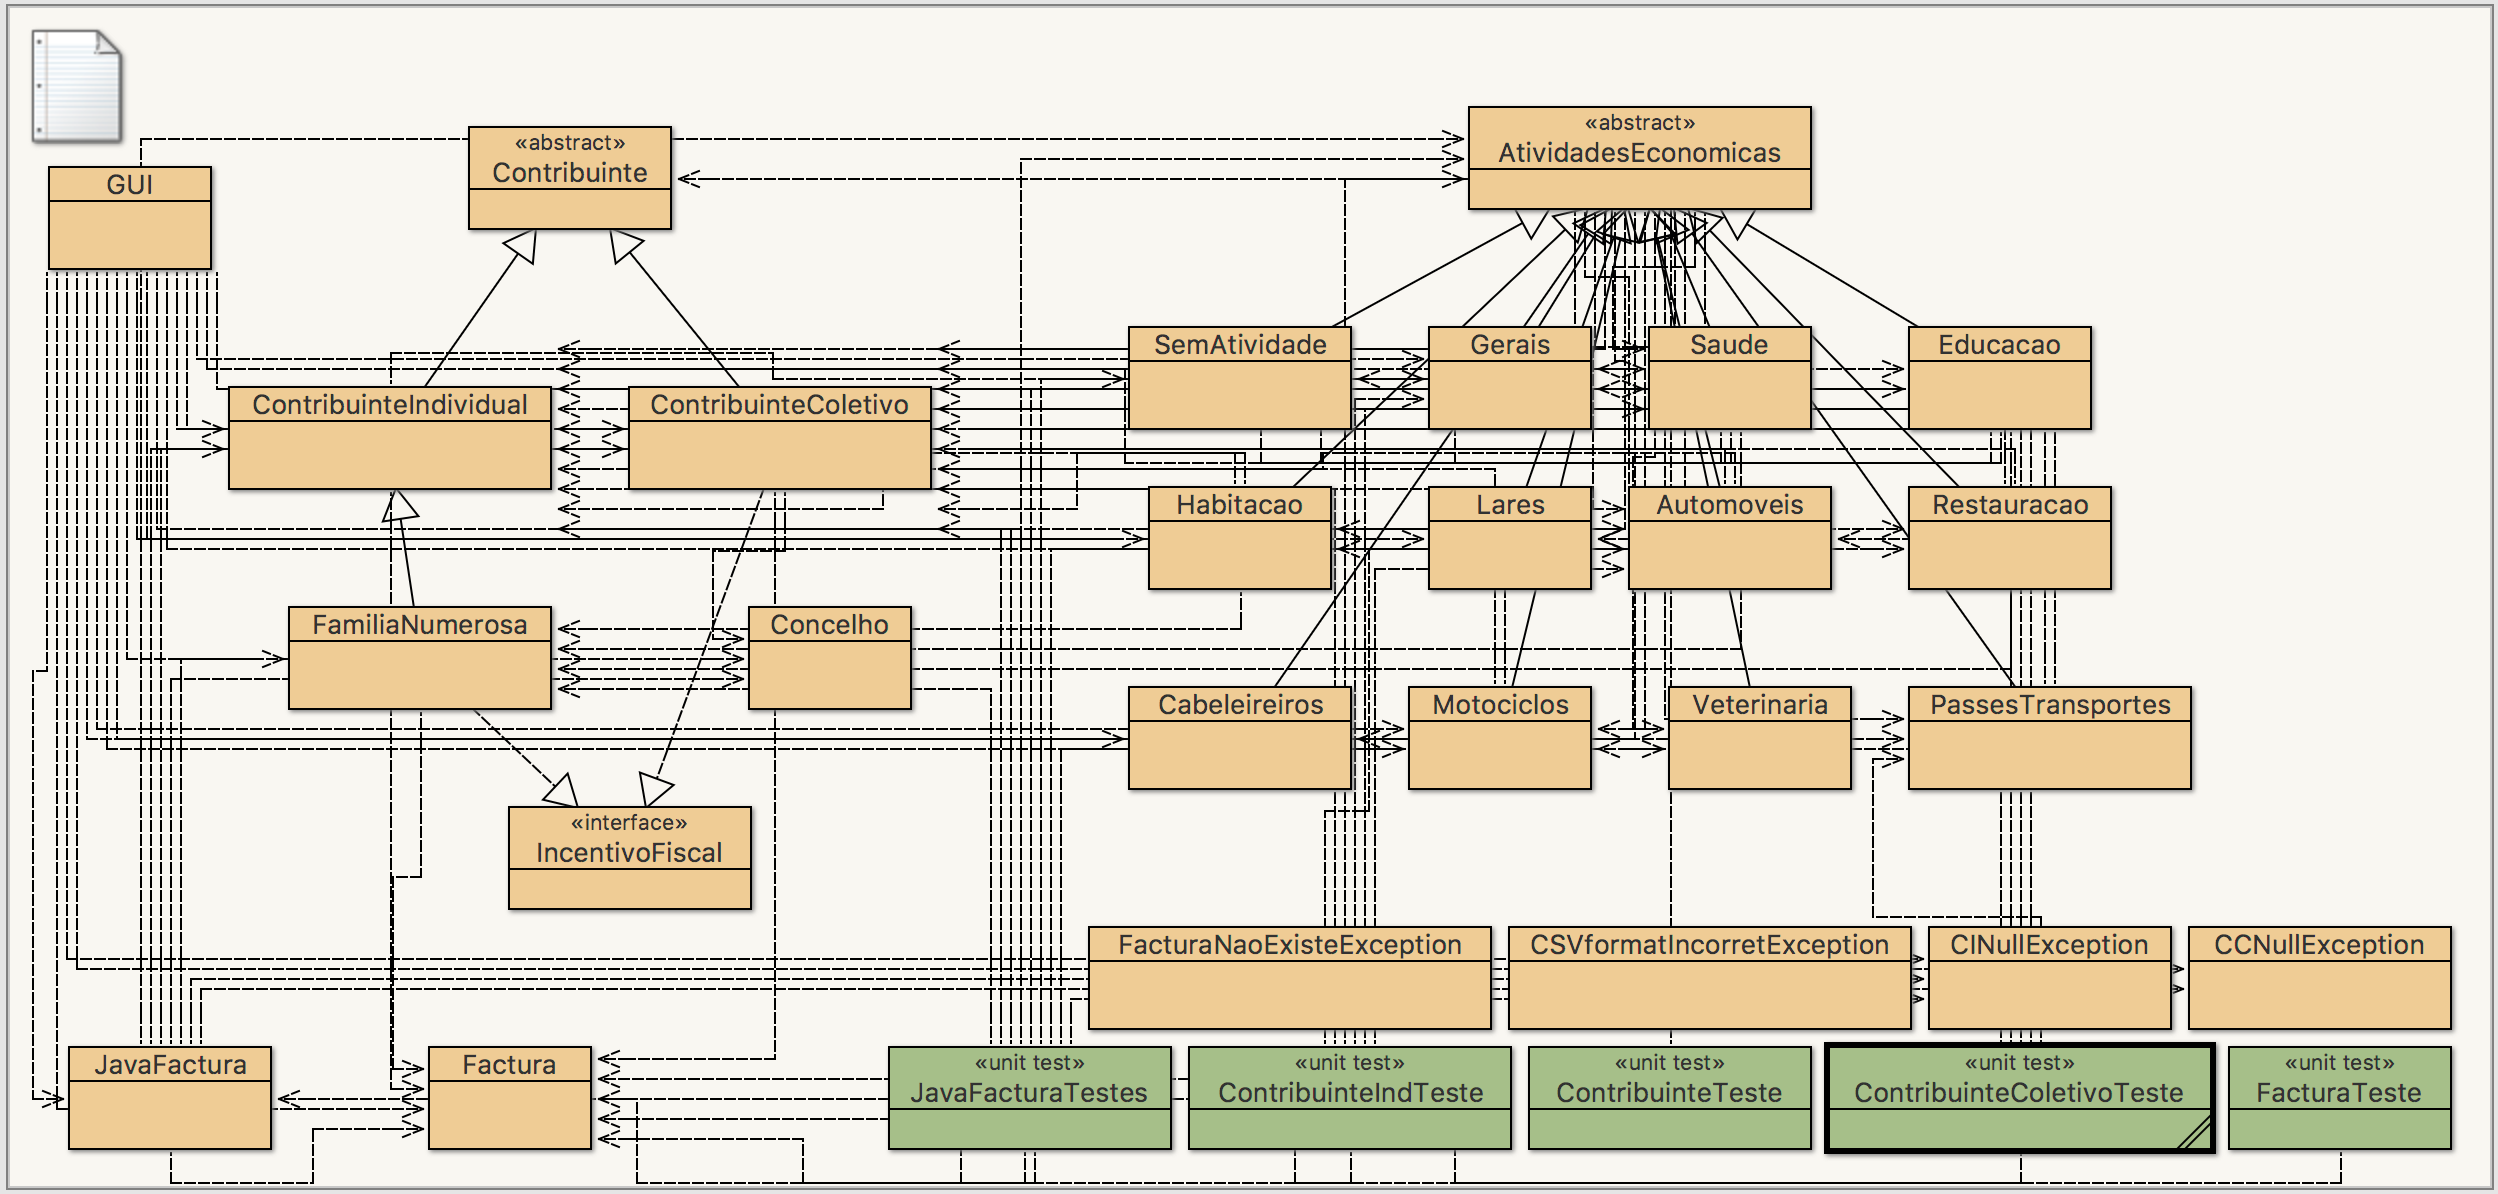
\includegraphics[scale=0.35]{imgs/classesbluej.png}
\caption{Imagem das classes BlueJ.}
\label{img:classesbluej}
\end{figure}


\subsection{Contribuinte}
\label{sec:contribuinte}

A classe \emph{Contribuinte} é uma classe abstrata que tem as seguintes
variáveis de instância:

\begin{verbatim}
private int NIF;
private String email;
private String nome;
private String morada;
private String password;
\end{verbatim}

\vspace{0.2cm}

O \textsf{NIF}, \textsf{email}, \textsf{nome}, \textsf{morada} e
\textsf{password} são atributos essenciais (informação comum)
a todos os contribuintes (tanto coletivos como individuais) pelo que
consideramos que seria mais útil e intuitivo elaborar esta classe abstrata.



\subsubsection{Contribuinte Individual}
\label{sec:contribuinteindividual}

A classe \emph{ContribuinteIndividual}, extensão da classe \emph{Contribuinte},
apresenta outras variáveis de instância que complementam a informação necessária
para identificar um contribuinte individual:

\begin{verbatim}
private int n_direcao;
private int n_dependentes;
private List<Integer> nifsDependentesAgregado;
private List<Integer> nifsDirecaoAgregado;
private double coeficiente_fiscal;
private Map<Integer, ArrayList<Factura>> grupos_facturas;
\end{verbatim}

\vspace{0.2cm}

A variável \textsf{n\_direcao} traduz o número de pessoas que constituem a
direção do agregado familiar (no máximo 2 contribuintes) e a variável \textsf{n\_dependentes}
traduz o número de dependentes do agregado (não há limite estipulado).

As listas de inteiros \textsf{nifsDependentesAgregado} e
\textsf{nifsDirecaoAgregado} armazenam os NIFs dos dependentes e dos
contribuintes a quem cabe a direção do agregado familiar, respetivamente.

A variável \textsf{coeficiente\_fiscal} guarda o coeficiente fiscal para efeitos
de dedução (fator multiplicativo que é associado a cada despesa elegível). O valor
do coeficiente fiscal é de uma unidade, à qual acresce uma décima (0,1) por cada pessoa que
integre o agregado familiar. Esta variável será tida em conta no cálculo das
deduções do indivíduo e do respetivo agregado.

Por último, temos um ``map'' \textsf{grupos\_facturas} onde a chave é o número
que identifica o setor de atividade económica (no nosso programa cada setor
corresponde a um número pré-definido, de 0 (sem atividade) até 11),  e o valor
corresponde a um \textsf{ArrayList} de faturas. Deste modo,
através do código que identifica a atividade económica temos acesso a todas as
faturas emitidas a um determinado contribuinte individual por setor económico.

\subsubsection{FamiliaNumerosa}
\label{sec:familianumerosa}

A classe \emph{FamiliaNumerosa}, extensão da classe \emph{ContribuinteIndividual},
tem uma única variável, a qual é uma variável de classe. Optamos por criar uma
única variável porque esta classe difere da de ContribuinteIndividual somente no
número de dependentes que integram um agregado familiar para efeitos fiscais.
Nessa medida, uma instância de FamiliaNumerosa tem todos os atributos de um contribuinte
individual e a caraterística de ter mais de 4 dependentes. Assim, a variável
criada define o limite inferior do número de dependentes desta classe e optamos
por classificá-la como sendo de classe e não de instância porque todos os objetos
desta classe partilham obrigatoriamente o referido limite inferior.
Ademais, esta classe foi criada para implementar o interface \emph{IncentivoFiscal},
o qual possui um único método, \emph{reducaoImposto}. Este método é definido nesta
classe e concede uma bonificação de 5\% por cada dependente que integra o agregado.



\vspace{0.2cm}


\subsubsection{Contribuinte Coletivo}
\label{sec:contribuintecoletivo}

A classe \emph{ContribuinteColetivo}, extensão da classe \emph{Contribuinte},
apresenta outras variáveis de instância que complementam a informação necessária
para identificar um contribuinte coletivo:

\begin{verbatim}
private List<Integer> atividades_economicas;
private double fator_deducao_fiscal;
private String concelho;
private List<Factura> facturas;
\end{verbatim}

\vspace{0.2cm}

Para além das variáveis de instância definidas em \emph{Contribuinte},
o contribuinte coletivo possui ainda uma lista de inteiros
(\textsf{atividades\_economicas}) onde estão armazenados
os códigos das atividades económicas onde a empresa se insere (1 no mínimo e
11 no máximo). A variável \textsf{fator\_deducao\_fiscal} que representa o fator
que a empresa tem no cálculo da dedução fiscal. O \textsf{concelho} que guarda o nome do concelho
onde se localiza a sede da empresa. Esta informação é necessária uma vez que as
empresas do interior terão um benefício extra associado.
Finalmente, também possui ainda uma lista de \textsf{facturas} com todas as faturas
emitidas pelo contribuinte coletivo.



\subsection{Factura}
\label{sec:fatura}

A classe \emph{Factura} apresenta as seguintes variáveis de instância, que são
necessárias para a representação de uma fatura:

\begin{verbatim}
private int id;
private int nif_emitente;
private String designacao;
private LocalDate data;
private int nif_cliente;
private String descricao;
private int natureza;
private BigDecimal valor;
List<Integer> historico_caes;
\end{verbatim}

\vspace{0.2cm}

Cada fatura é identificada através do seu \textrm{id},
o qual é único e fixado de forma sequencial, aquando da emissão da fatura e
armazenado na variável \textsf{id}.
O \textrm{NIF do contribuinte coletivo} que emitiu a fatura está identificado na
variável \textsf{nif\_emitente}. A \textsf{designacao} guarda a firma do emitente; a \textsf{data}
indica a data em que a fatura foi emitida, no formato \textrm{LocalDate}; o
\textsf{nif\_cliente}, refere-se ao nif do contribuinte a quem a fatura foi emitida;
 a \textsf{descricao} da fatura é o campo onde se identifica o tipo de bem ou serviço
transacionado e o \textsf{valor}, expresso no formato \textrm{BigDecimal}, é o
valor da despesa efetuada pelo contribuinte.

Para além disso, cada fatura contém a sua \textsf{natureza}, a qual corresponde ao setor
de atividade da empresa ou, no caso da empresa emitente ter mais do que um setor
de atividade associado, a natureza assumirá o valor de zero até que o contribuinte
associe o setor de atividade correspondente, classificando a despesa de acordo com
a sua natureza correta.
No caso do contribuinte não associar a despesa ao correto setor de atividade da empresa,
a fatura não será considerada para efeitos fiscais, não obstante
a fatura que identifica a despesa continua a estar associada ao contribuinte individual.


Por último, a fatura tem ainda uma lista de inteiros com o histórico dos setores
de atividade (\textsf{historico\_caes}) da fatura.
Note-se que se a empresa só tiver um setor de atividade, a classificação da
atividade económica (CAE) constante da fatura nunca pode ser alterada,
pelo que a referida lista sempre é vazia.
No entanto, se a empresa tiver mais do que um setor de atividade económica,
o CAE de todas as faturas emitidas por si começa por ser 0 (sem atividade definida),
informação que também é conservada no histórico da fatura. Aquando da alteração do
CAE, por parte do contribuinte individual, o novo código do setor é adicionado
à lista \textsf{historico\_caes}.

\vspace{0.2cm}

É de salientar que as \textbf{faturas são partilhadas} entre os contribuintes individuais
e os contribuintes coletivos, ou seja, por exemplo, se o contribuinte individual
alterar o CAE da fatura o contribuinte coletivo terá conhecimento.


\subsection{Concelho}
\label{sec:concelho}

\begin{verbatim}
private String nome;
private double beneficio;
\end{verbatim}

\begin{verbatim}
static private Map<String, Concelho> concelhos;
\end{verbatim}

Esta classe foi criada para que determinados concelhos possam conceder
um incentivo fiscal. De facto, o que se pretendeu foi criar uma lista de concelhos
de Portugal Continental e associar a determinados concelhos, os do interior do
país, um beneficio fiscal que será concedido ao contribuinte
que compre um bem ou adquira um serviço a uma empresa sediada num concelho do interior.
Esta classe possui duas variáveis de instância, \textsf{nome}, \textsf{beneficio}.
A primeira indica o nome do concelho em questão e a segunda o benefício fiscal que
lhe está associado.
Além destas duas variáveis, esta classe contém uma variável de classe
\textsf{concelhos}, que representa uma hashmap de todos os concelhos existentes
na nossa aplicação, sendo a chave dessa mesma hashmap o nome do concelho.


\subsection{Atividades Económicas}
\label{sec:atividadeseconomicas}

A necessidade da criação desta classe abstrata surgiu para que fosse mais fácil
incluir novos tipos de despesas passíveis de dedução, sendo, por isso, mais eficaz
criar uma classe superior que encerra os atributos comuns a todas as atividades,
mas que não pode ser instanciada, e criar as diversas subclasses que descrevem
o estado e o comportamento de cada uma das atividades económicas existentes que dão
direito a dedução.

A classe \emph{AtividadesEconomicas} é uma classe abstrata que tem as seguintes
variáveis de instância:

\begin{verbatim}
private int codigo;
private String setor;
private double percentagem_deducao;
private BigDecimal limite_deducao;
static private Map<Integer, AtividadesEconomicas> atividades;
\end{verbatim}

\vspace{0.2cm}

O \textsf{código} da atividade económica é um número pré-definido por nós para
cada um dos setores, de modo a simplificar a sua utilização no programa.
O \textsf{setor} armazena o nome da atividade económica.

A \textsf{percentagem\_deducao} e o \textsf{limite\_deducao} estabelecem,
respetivamente, a percentagem e o limite de dedução de cada atividade económica.
Convém referir que o limite das deduções é aplicável às despesas suportadas por
cada um dos indivíduos que compõem o agregado familiar. Por outras palavras, cada
membro do agregado familiar pode beneficiar de deduções até ao máximo definido
para cada atividade económica.

Finalmente, implementamos uma variável de classe \textsf{atividades}, isto é,
variável comum a todas as instâncias da classe, que representa uma hashmap de
todas as atividades económicas, sendo que o setor económico de uma empresa terá
de pertencer, obrigatoriamente, a uma ou várias destas atividades pré-definidas.
Esta variável permite-nos guardar as informações que dizem respeito à globalidade
das instâncias criadas de atividades.



\subsubsection{Subclasses Económicas}
\label{sec:sematividade}

A classe \emph{SemAtividade} será utilizada nas faturas que não têm
CAE definido logo à partida (faturas que foram emitidas por empresas que têm
mais do que uma atividade económica).
Esta "atividade" terá o \textsf{código} 0 no nosso programa.

\begin{verbatim}
public static final SemAtividade objeto = new SemAtividade();
\end{verbatim}

Possui uma única variável que é de classe porque queremos uma única instância
daquela classe no programa. Entretanto, essa variável encontra-se desde logo
inicializada com os valores do código, do setor, da percentagem de dedução e
do limite de dedução, todos eles atributos herdados da classe superior
AtividadesEconomicas por razões de pragmaticidade, já que são imutáveis.
De ressaltar que este procedimento verifica-se em todas as classes referente
às atividades económicas criadas, mudando somente os valores dos referidos atributos.

\vspace{0.2cm}

Na classe \emph{SemAtividade}, o código é o zero, o setor designa-se por Sem
Atividade, a percentagem de dedução e o limite da dedução são ambos zero.

\vspace{0.2cm}

Na classe \emph{Despesas Gerais Familiares}, o código é o um, o setor tem a
designação de Gerais, a percentagem de dedução é de 35\% sobre a despesa e o
limite é de 100 euros.

\vspace{0.2cm}

Na classe \emph{Saúde}, o código é o dois, o setor tem a mesma
designação, a percentagem de dedução é de 15\% sobre a despesa e o
limite é de 400 euros.

\vspace{0.2cm}

Na classe \emph{Educação}, o código é o três, o setor tem a mesma
designação, a percentagem de dedução é de 30\% sobre a despesa e o
limite é de 400 euros.

\vspace{0.2cm}

Na classe \emph{Habitação}, o código é o quatro, o setor tem a mesma
designação, a percentagem de dedução é de 15\% sobre a despesa e o
limite é de 400 euros.

\vspace{0.2cm}

Na classe \emph{Lares}, o código é o cinco, o setor tem a mesma
designação, a percentagem de dedução para este setor é de 25\% sobre a despesa
e o limite da dedução é de 400 euros.

\vspace{0.2cm}

Na classe \emph{Reparação de Automóveis}, o código é o seis, a
designação é Automoveis, a percentagem de dedução é de 5\% sobre a despesa e o
limite é de 100 euros.

\vspace{0.2cm}

Na classe \emph{Restauração e Alojamento}, o código é o sete, a
designação é Restauracao, a percentagem de dedução é de 5\% sobre a despesa e o
limite é de 100 euros.

\vspace{0.2cm}

Na classe \emph{Cabeleireiros}, o código é o oito, o setor tem a mesma
designação, este setor não dá direito a qualquer tipo de dedução e, por isso,
também não tem limite dedutível.

\vspace{0.2cm}

Na classe \emph{Motociclos}, o código é o nove, o setor tem a mesma
designação, a percentagem de dedução é de 5\% sobre a despesa e o
limite é de 100 euros.

\vspace{0.2cm}

Na classe \emph{Atividades Veterinárias}, o código é o dez, o setor tem a
designação de Veterinarias, a percentagem de dedução é de 5\% sobre a despesa e o
limite é de 100 euros.

\vspace{0.2cm}

Finalmente, a classe \emph{PassesTransportes} é a atividade com o código onze,
o setor tem a designação de PassesTransportes, o limite da dedução
para este setor é 100 euros e a percentagem de dedução é de 5\% sobre o valor da despesa.

\vspace{0.2cm}

Os valores de percentagem de dedução, assim como o limite acima referidos são essenciais
para o cálculo do montante das deduções do contribuinte, bem como do seu agregado
familiar. Outros fatores determinantes no cálculo destes montantes são o coeficiente
fiscal do contribuinte, o número de elementos do agregado familiar e a sede da empresa que presta
o serviço ou vende o bem.
Ora, entendemos que o cálculo desse valor deveria variar em função da atividade económica,
já que as despesas feitas pelo contribuinte devem ter tratamento diferente consoante
a natureza da mesma.\par


A classe de Cabeleireiros não confere nenhum tipo de beneficio fiscal. \par


No caso das atividades das classes Gerais, Lares e Veterinaria o cálculo das deduções
de cada elemento do agregado familiar é feito multiplicando o valor da despesa pelo
coeficiente fiscal e pela percentagem da dedução prevista para cada uma dessas atividades
até ao limite de dedução previsto. \par


Por seu turno, no caso dos setores de atividade como a Saúde, a Educação e a
Habitação, o cálculo do montante dos valores a deduzir tem em consideração o número
de dependentes que integram o agregado familiar. De facto, se o contribuinte contrair uma
despesa relativa a um desses setores de atividade e pertencer a uma família numerosa, o
cálculo da dedução far-se-á nos termos anteriormente descritos, mas o limite
da dedução inicialmente previsto aumenta. Esse aumento varia de acordo com o número de
dependentes, o limite é majorado em 5\% por cada dependente. Por exemplo, um
elemento de uma família com 5 dependentes que tenha contraído uma despesa de saúde
verá o seu limite de dedução do setor aumentar da seguinte forma:

\begin{equation} 5\% * 5 * 400 = 100 \end{equation}


 \begin{equation} 400 + 100 = 500 \end{equation}

Assim, as despesas de saúde passam a ter um novo limite de dedução que ascende a 500 euros
para cada elemento do agregado familiar.


No caso das restantes atividades económicas, automóveis, motociclos, restauração
e passes de transportes, o cálculo das deduções está relacionado com a sede da
empresa que presta o serviço. Efetivamente, neste caso o valor deduzido em cada
transação varia de acordo com a localização da sede da empresa, já que se a
empresa que emitiu a fatura estiver sediada num concelho do interior, a percentagem
de dedução aumenta, de acordo com o benefício estipulado na classe Concelho.



\subsection{EmpresasTop}
\label{sec:empresastop}

Esta classe foi criada dentro do interface gráfico, visto que somente é necessária
para apresentar a listagem das empresas com mais faturas do sistema e respetivos
valores de despesas e de deduções.



\subsection{JavaFactura}
\label{sec:javafatura}

Esta classe é provavelmente a classe crucial para a realização do trabalho
uma vez que uma grande maioria das funções utilizadas para a realização dos
requisitos propostos se encontram explicitadas nesta classe. Todas essas
implementações serão devidamente apresentadas na Secção~\ref{sec:implementacao}.

Assim, para guardar os dois principais atores do sistema recorremos ao uso de
dois ``maps'', um para armazenar os contribuintes \textsf{individuais}
e outro para armazenar os contribuintes \textsf{coletivos}:

\begin{verbatim}
private Map<Integer, ContribuinteIndividual> individuais;
private Map<Integer, ContribuinteColetivo> coletivos;
\end{verbatim}

\vspace{0.2cm}

A chave para ambos os ``maps'' é o NIF, dos individuais para o caso dos individuais,
e dos coletivos no caso dos coletivos.



\section{Interfaces}
\label{sec:interfaces}

A ponto de colmatar um dos últimos requisitos surgiu a necessidade de criar uma
interface, explicada em seguida:



\subsection{Incentivo Fiscal}
\label{sec:incentivofiscal}

Este interface possui apenas um método, \emph{reducaoImposto}, comum às classes
FamiliaNumerosa e ContribuinteColetivo, porquanto tenta relacionar essas
duas classes, criando um novo tipo de dados que serão os objetos de instância dessa
classe que têm um único comportamento, a redução do imposto.
Por um lado, a familia numerosa estabelece uma redução de imposto,
prevendo uma bonificação de cinco por cento por cada dependente que integre o agregado.
Por outro lado, o contribuinte coletivo implementa esse mesmo método,
\emph{reducaoImposto}, fazendo depender o calculo da dedução da localização
da sua sede.
Assim, e conforme já explicamos anteriormente, este método tem um papel
determinante no cálculo das deduções do contribuinte, bem como das do seu agregado familiar.



\section{Classes de Exceções}
\label{sec:excecoes}

A ponto de exceções que eventualmente poderão acontecer no programa desenvolvemos
duas classes de \emph{Exception} de modo a conseguirmos tratar de forma adequada
estes ``bugs'' que poderão surgir e de separar código de tratamento de erros de
código regular.



\subsection{CINullException}
\label{sec:cinullexception}

A classe \emph{CINullException} diz respeito a quando um
contribuinte individual a que tentamos aceder não existe (é null).



\subsection{CCNullException}
\label{sec:ccnullexception}

A classe \emph{CCNullException} diz respeito a quando um
contribuinte coletivo a que tentamos aceder não existe (é null).



\subsection{FacturaNaoExisteException}
\label{sec:FacturaNaoExiste}

A classe \emph{FacturaNaoExisteException} diz respeito a quando uma
factura a que se tenta aceder não existe (é null).



\subsection{CSVformatIncorretException}
\label{sec:CSVformatIncorret}

A classe \emph{CSVformatIncorretException} é usada quando ao importar um
ficheiro CSV a linha a ser analisada não contém informação de um objeto que
pertença à aplicação.



\section{Implementação e Manual de Utilizador}
\label{sec:implementacao}

Para a concretização do trabalho prático, e com a extrema ajuda das classes já
mencionadas, respondemos a todos os requisitos do trabalho prático.

Como já foi referido, recorremos à biblioteca \emph{javafx} para representar
a interface gráfica do programa e todos os métodos efetuados para tal encontram-se
na classe \textsf{GUI}.

Nas imagens que iremos apresentar o programa já se
encontra pré-populado com um conjunto de dados significativos, que permite
testar toda a aplicação.

É de salientar, mais uma vez, que a classe \textsf{JavaFactura} é a que contém
os ``maps'' com as informações dos contribuintes individuais e dos contribuintes coletivos,
que por sua vez armazenam as faturas.

O ponto de partida do programa é a Figura~\ref{img:ecrainicial}, onde os contribuintes
podem fazer login ou registarem-se, caso sejam individuais ou coletivos, carregando no
botão que mais lhes convêm.

\begin{figure}[H]
\centering
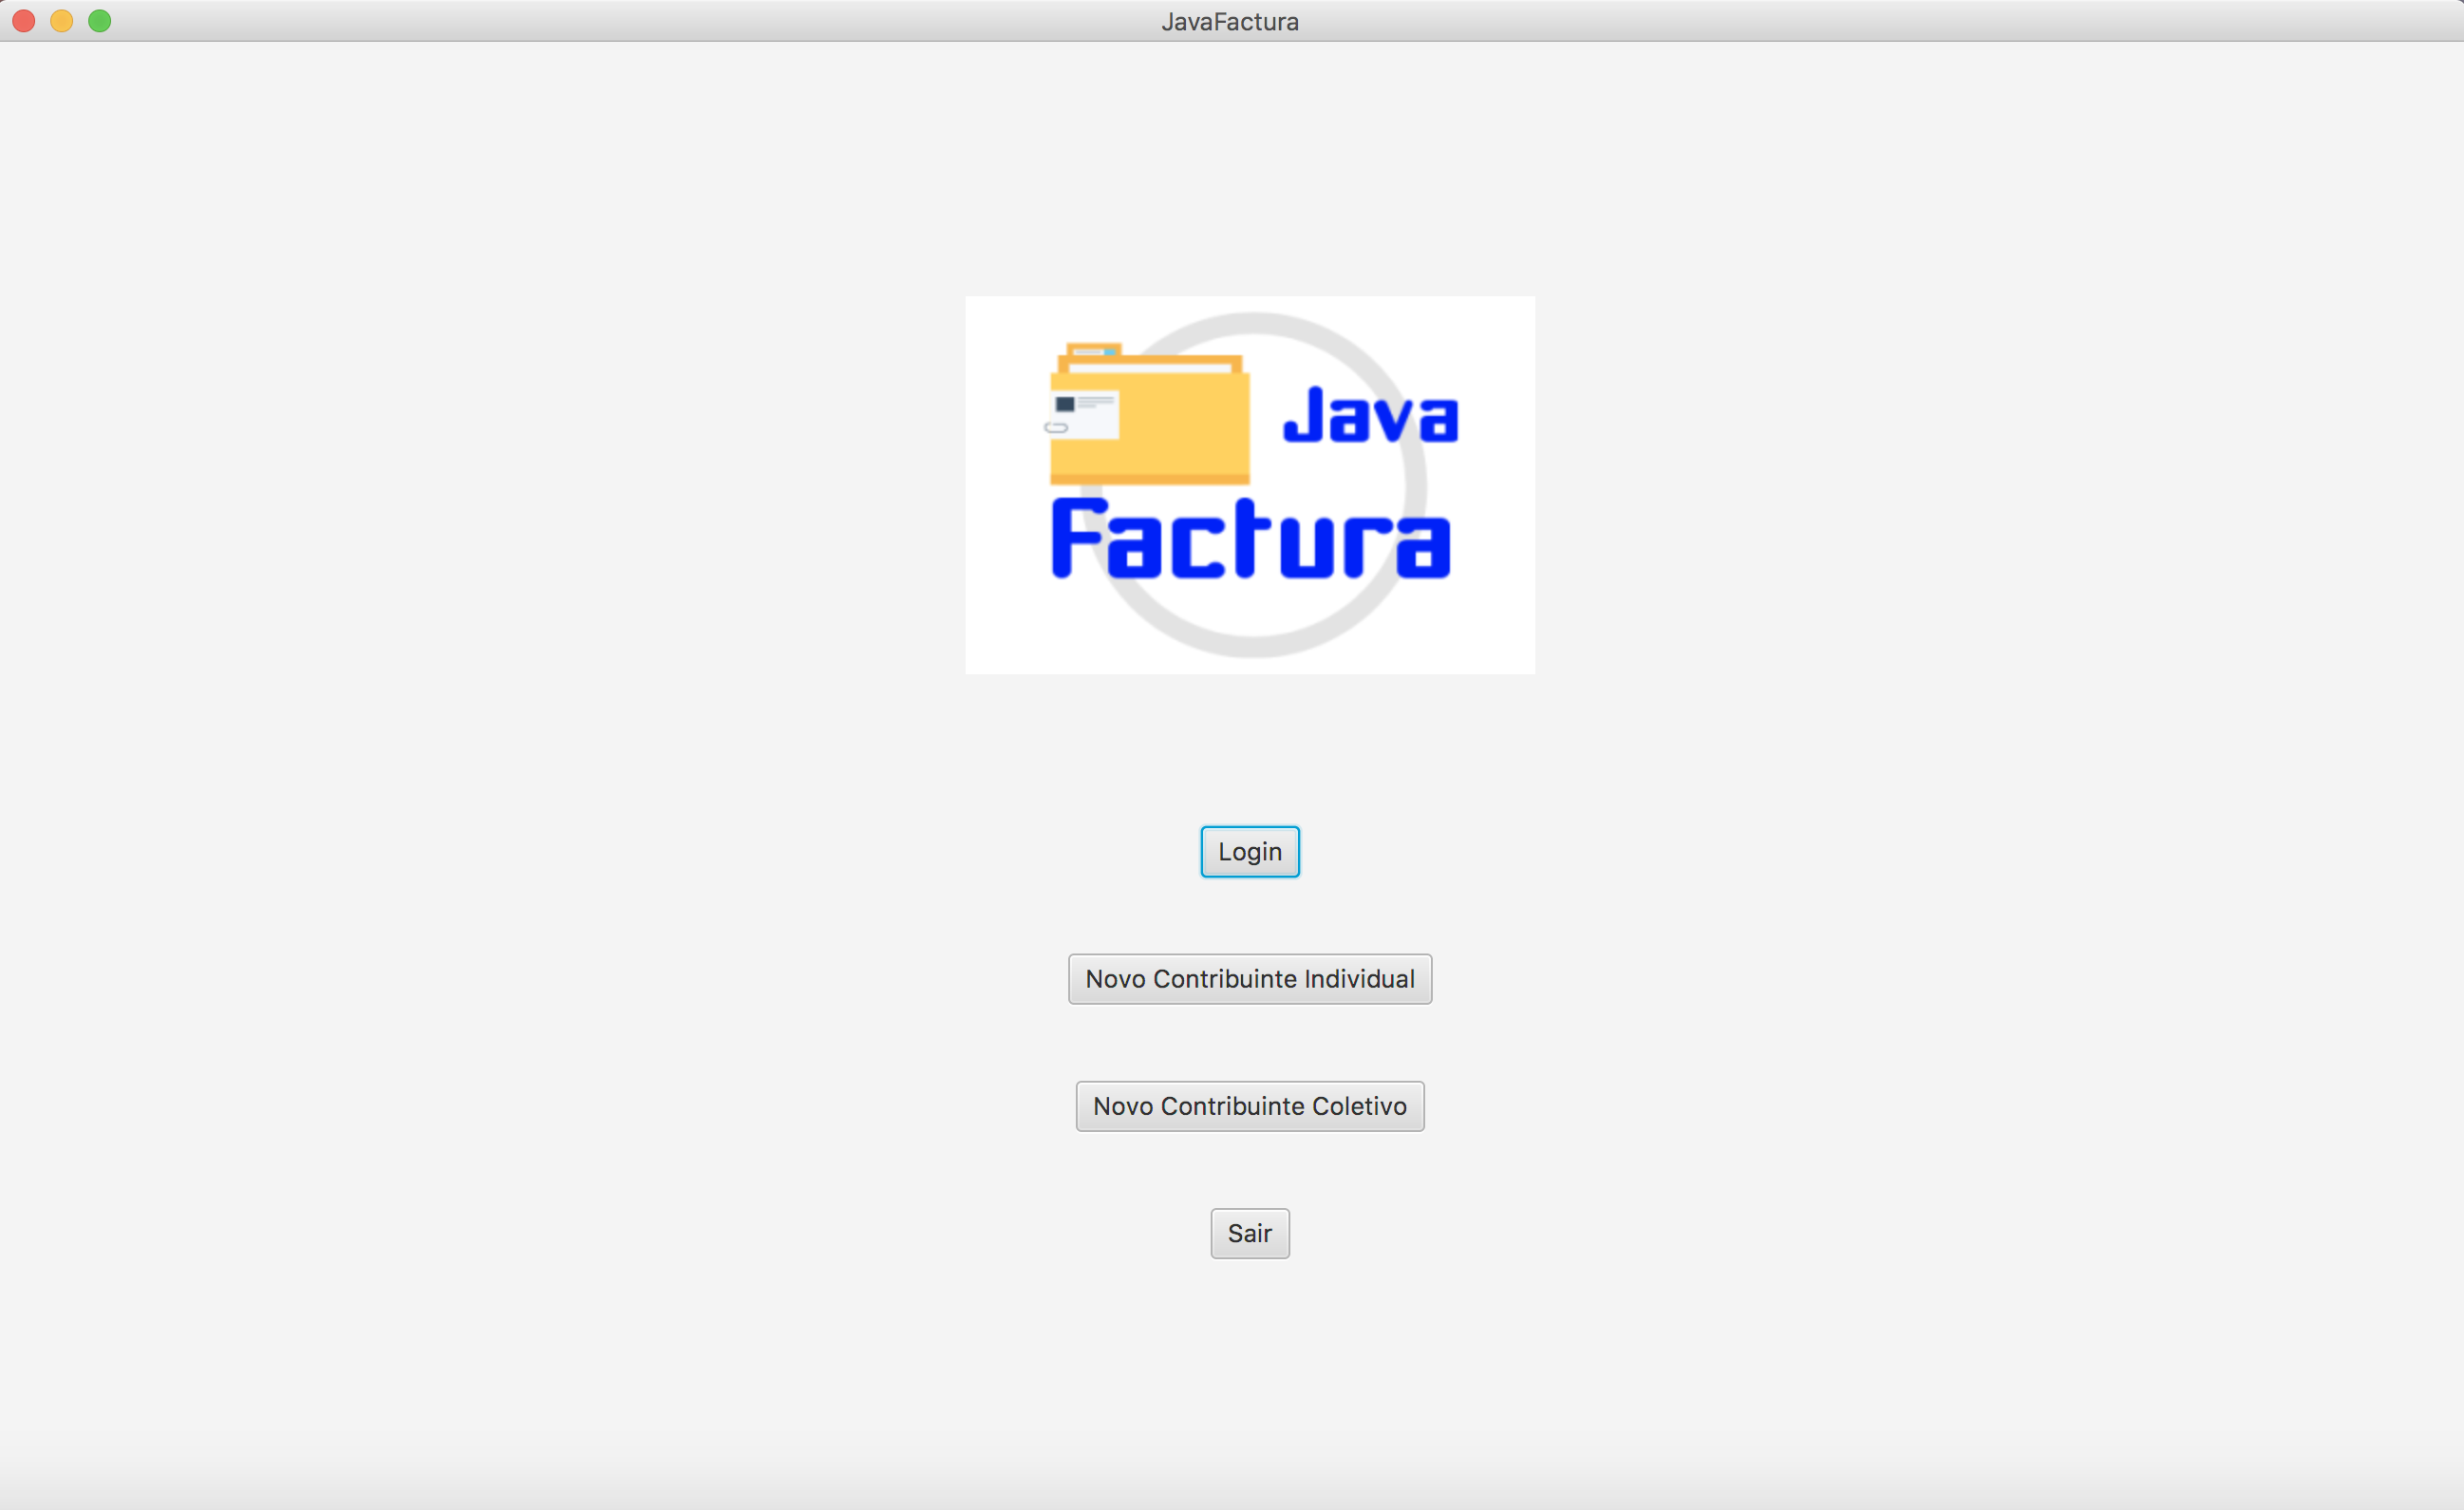
\includegraphics[scale=0.20]{imgs/ecrainicial.png}
\caption{Demonstração da página inicial do programa.}
\label{img:ecrainicial}
\end{figure}

Em seguida, explicamos a forma como resolvemos cada uma das questões e a respetiva
demonstração na aplicação:


\subsection{Registar Contribuintes}
\label{sec:registarcontribuintes}

\begin{itemize}

\item \textbf{Registar um contribuinte, quer seja individual ou empresa.}

De forma a responder ao ponto acima mencionado, depois do utilizador se deparar
com a Figura~\ref{img:ecrainicial}, se a intenção do mesmo for \textbf{registar um novo
contribuinte individual} aparecerá a Figura~\ref{img:criarci}.

\begin{figure}[H]
\centering
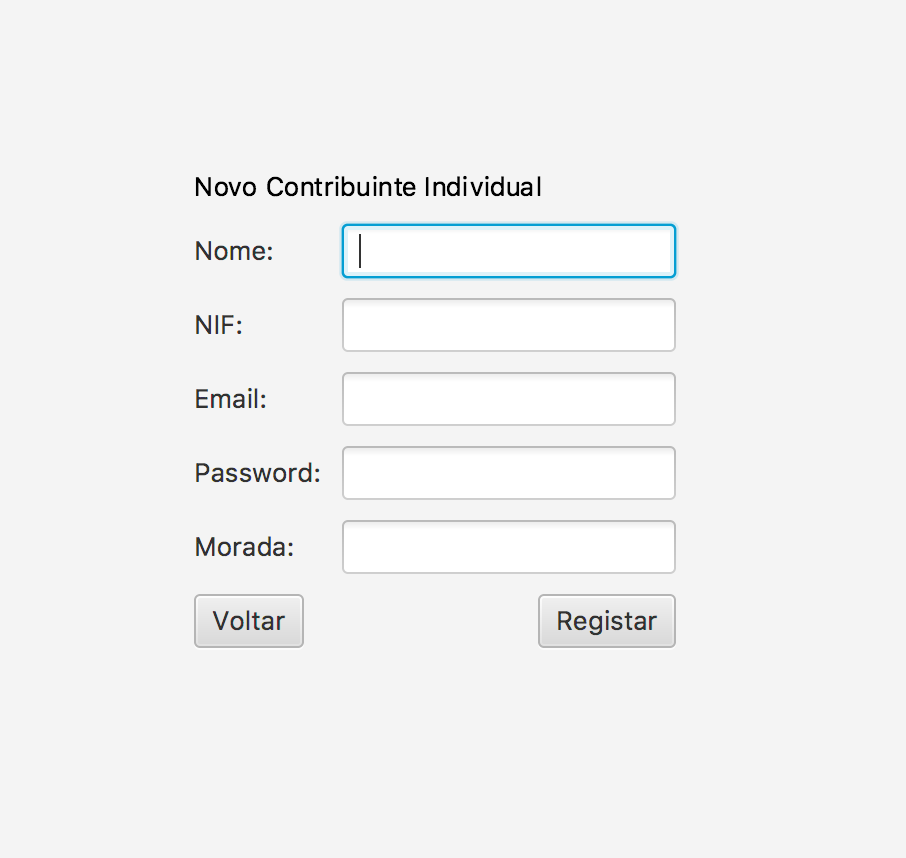
\includegraphics[scale=0.40]{imgs/criarci.png}
\caption{Registar um Contribuinte Individual.}
\label{img:criarci}
\end{figure}

Deste modo, o utilizador terá que preencher obrigatoriamente todos os campos e,
dentro do nosso programa, é chamado o contrutor parametrizado do contribuinte individual.
É adicionado ao respetivo ``map'', da classe \textsf{JavaFactura}, a informação
deste contribuinte individual criado, como mostra a Figura~\ref{img:criarci_func}.

\begin{figure}[H]
\centering
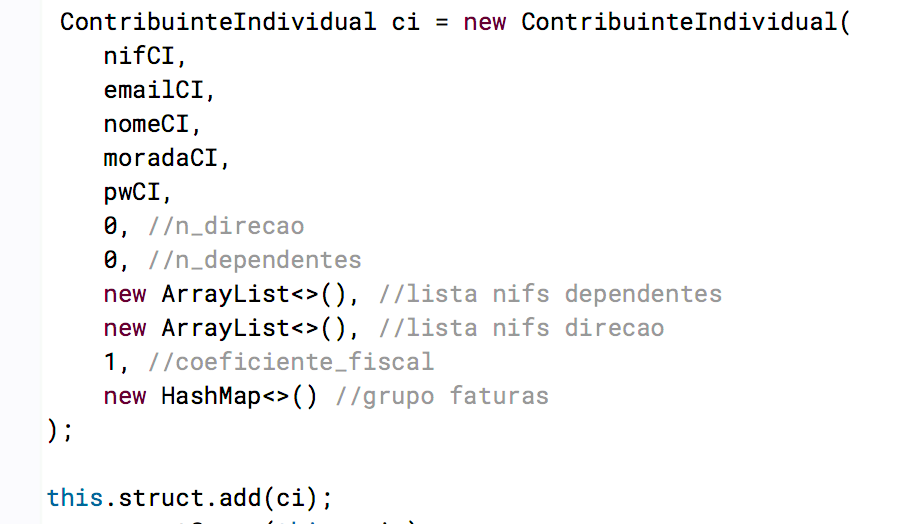
\includegraphics[scale=0.40]{imgs/criarci_func.png}
\caption{Registar um Contribuinte Individual (métodos).}
\label{img:criarci_func}
\end{figure}

Existem no nosso sistema de input output (classe \textsf{GUI})
``trys and catchs'' para perceber se o nif introduzido se trata de um número
e se o contribuinte que está a ser adicionado já não pertence ao sistema (quer
como contribuinte individual, quer como contribuinte coletivo).

Em caso de sucesso é enviada uma mensagem para o ecrã e em caso de insucesso também.


\vspace{0.4cm}


No caso da intenção do utilizador ser \textbf{registar um contribuinte coletivo} o raciocínio
utilizado é exatamente o mesmo. Aparece no ecrã do utilizador a seguinte janela
(Figura~\ref{img:criarcc}), e é igualmente obrigatório o utilizador preencher
todos os campos, inclusivé
o campo das atividades económicas, onde o contribuinte terá que escolher pelo menos um
dos setores de atividade, e no máximo todos eles (são 11 no total).

\begin{figure}[H]
\centering
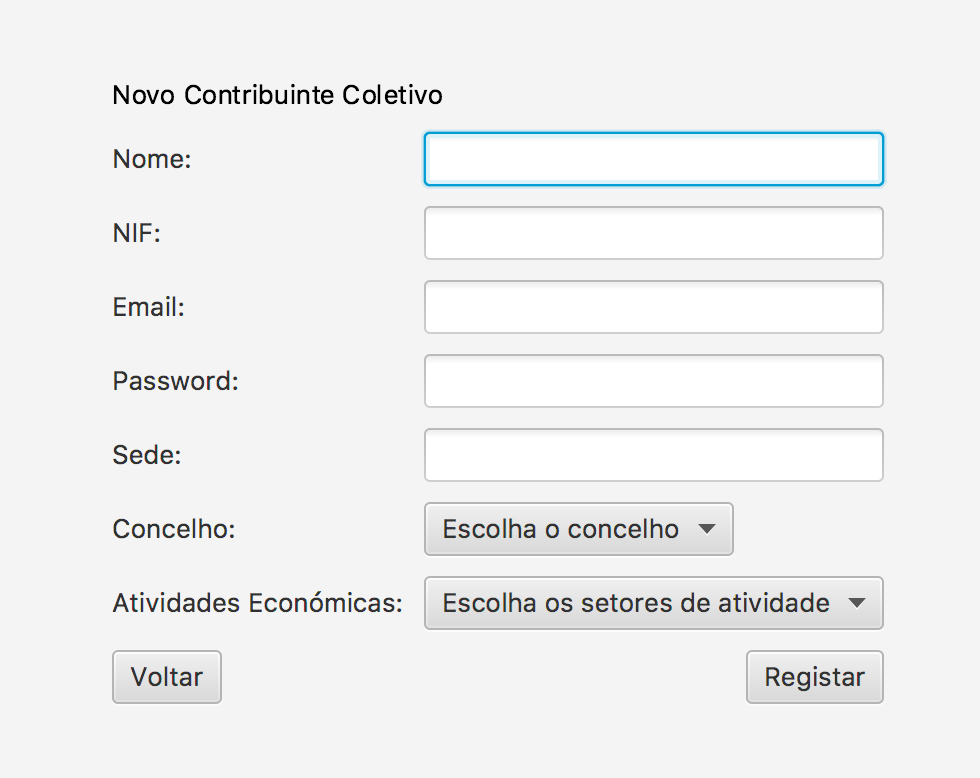
\includegraphics[scale=0.40]{imgs/criarcc.png}
\caption{Registar um Contribuinte Coletivo.}
\label{img:criarcc}
\end{figure}

No programa, é chamado o construtor parametrizado do contribuinte coletivo e as suas
informações são adicionadas ao ``map'' da classe \textsf{JavaFactura}.



\subsection{Login}
\label{sec:login}

\item \textbf{Validar o acesso à aplicação utilizando as credenciais (nif e password), por parte
de diferentes atores.}

Como já apresentado na Figura~\ref{img:ecrainicial}, se a intenção do utilizador
for efetuar login na aplicação aparacerá a figura apresentada em seguida, onde o
utilizador deverá preencher ambos os campos:

\begin{figure}[H]
\centering
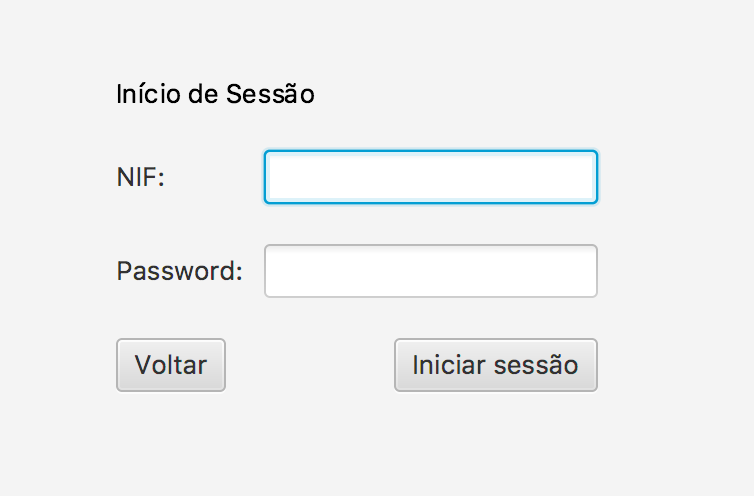
\includegraphics[scale=0.40]{imgs/login.png}
\caption{Login.}
\label{img:login}
\end{figure}

O nosso sistema possui três tipos de atores: Contribuintes
Individuais, Contribuintes Coletivos e o Administrador.

O Administrador possui um \textbf{NIF = 0} e uma \textbf{password = admin}.

Assim, no nosso sistema de input output é averiguado se foram introduzidas as
credenciais do administrador, e, caso afirmativo, o utilizador é enviado para a
respetiva dashboard (Figura~\ref{img:dashboardadmin}).

Caso não tenha sido o administrador a iniciar sessão, é necessário averiguar se
foi um contribuinte individual ou um contribuinte coletivo. Para isso, recorremos
às seguintes funções, sendo em primeiro lugar averiguado se foi um individual
(Figura~\ref{img:loginindividual}), e em segundo lugar se foi um coletivo
(Figura~\ref{img:logincoletivo}). Se não existir nenhuma entidade com as credenciais
inseridas é enviada uma mensagem de aviso ao utilizador.

\begin{figure}[H]
\centering
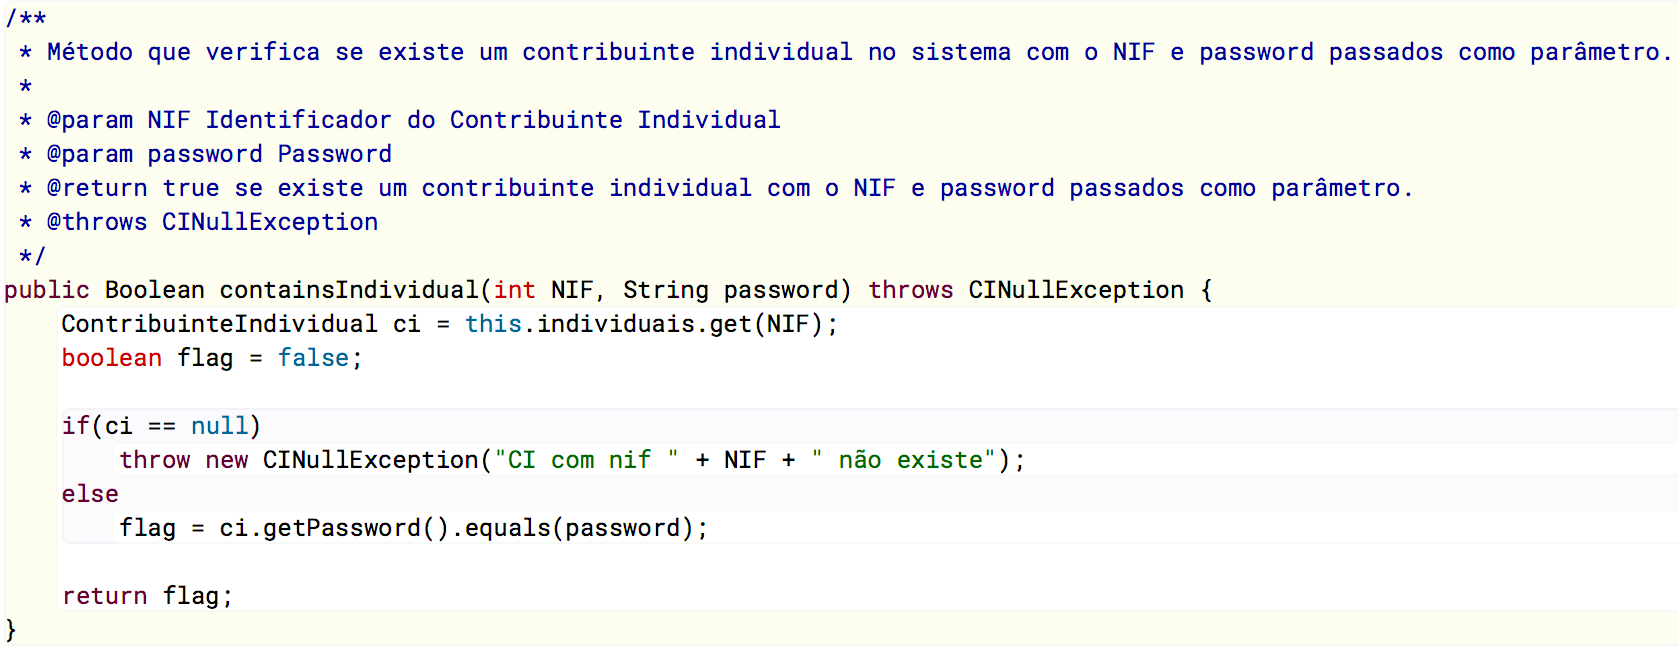
\includegraphics[scale=0.40]{imgs/loginindividual.png}
\caption{Login Contribuinte Individual.}
\label{img:loginindividual}
\end{figure}

\begin{figure}[H]
\centering
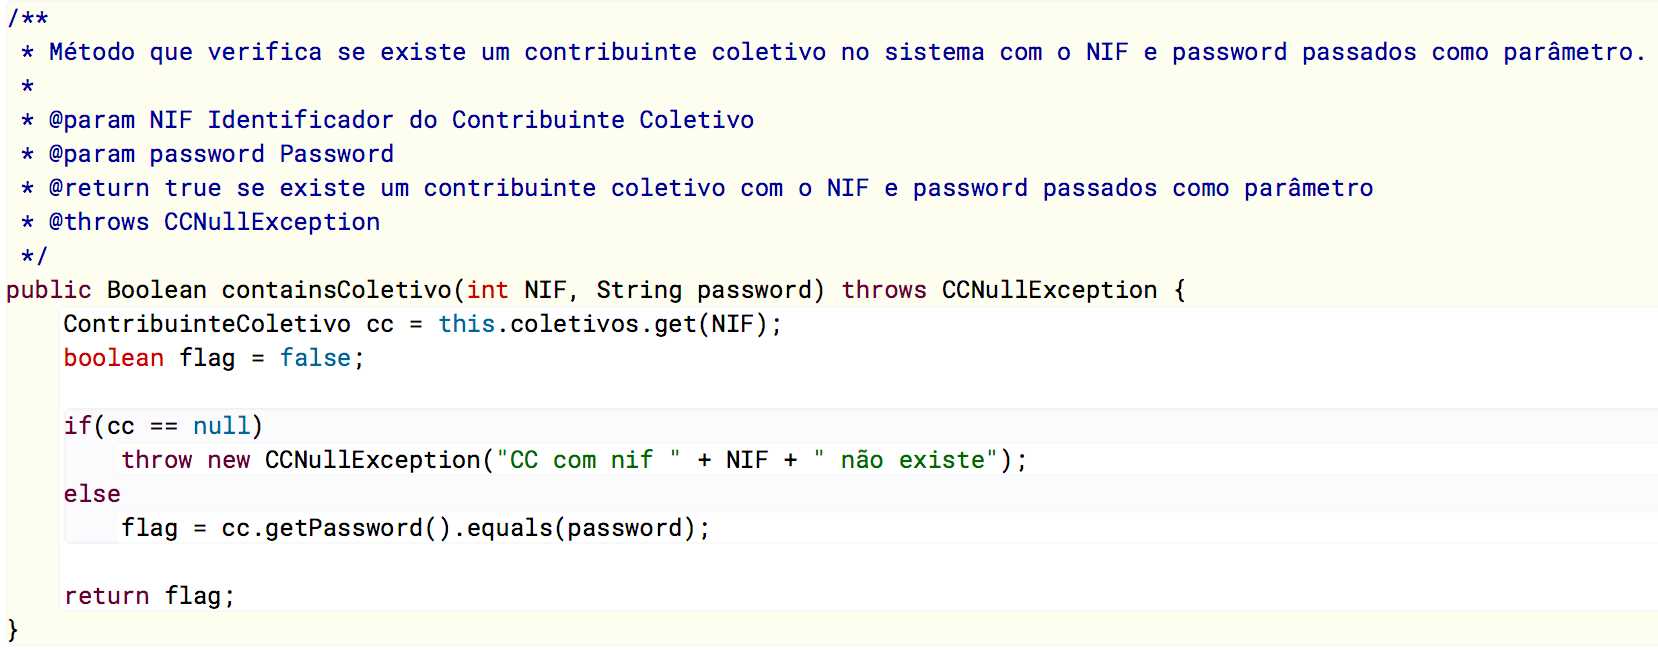
\includegraphics[scale=0.40]{imgs/logincoletivo.png}
\caption{Login Contribuinte Coletivo.}
\label{img:logincoletivo}
\end{figure}

Caso tenha sido um Contribuinte Individual é apresentada a seguinte dashboard:
\begin{figure}[H]
\centering
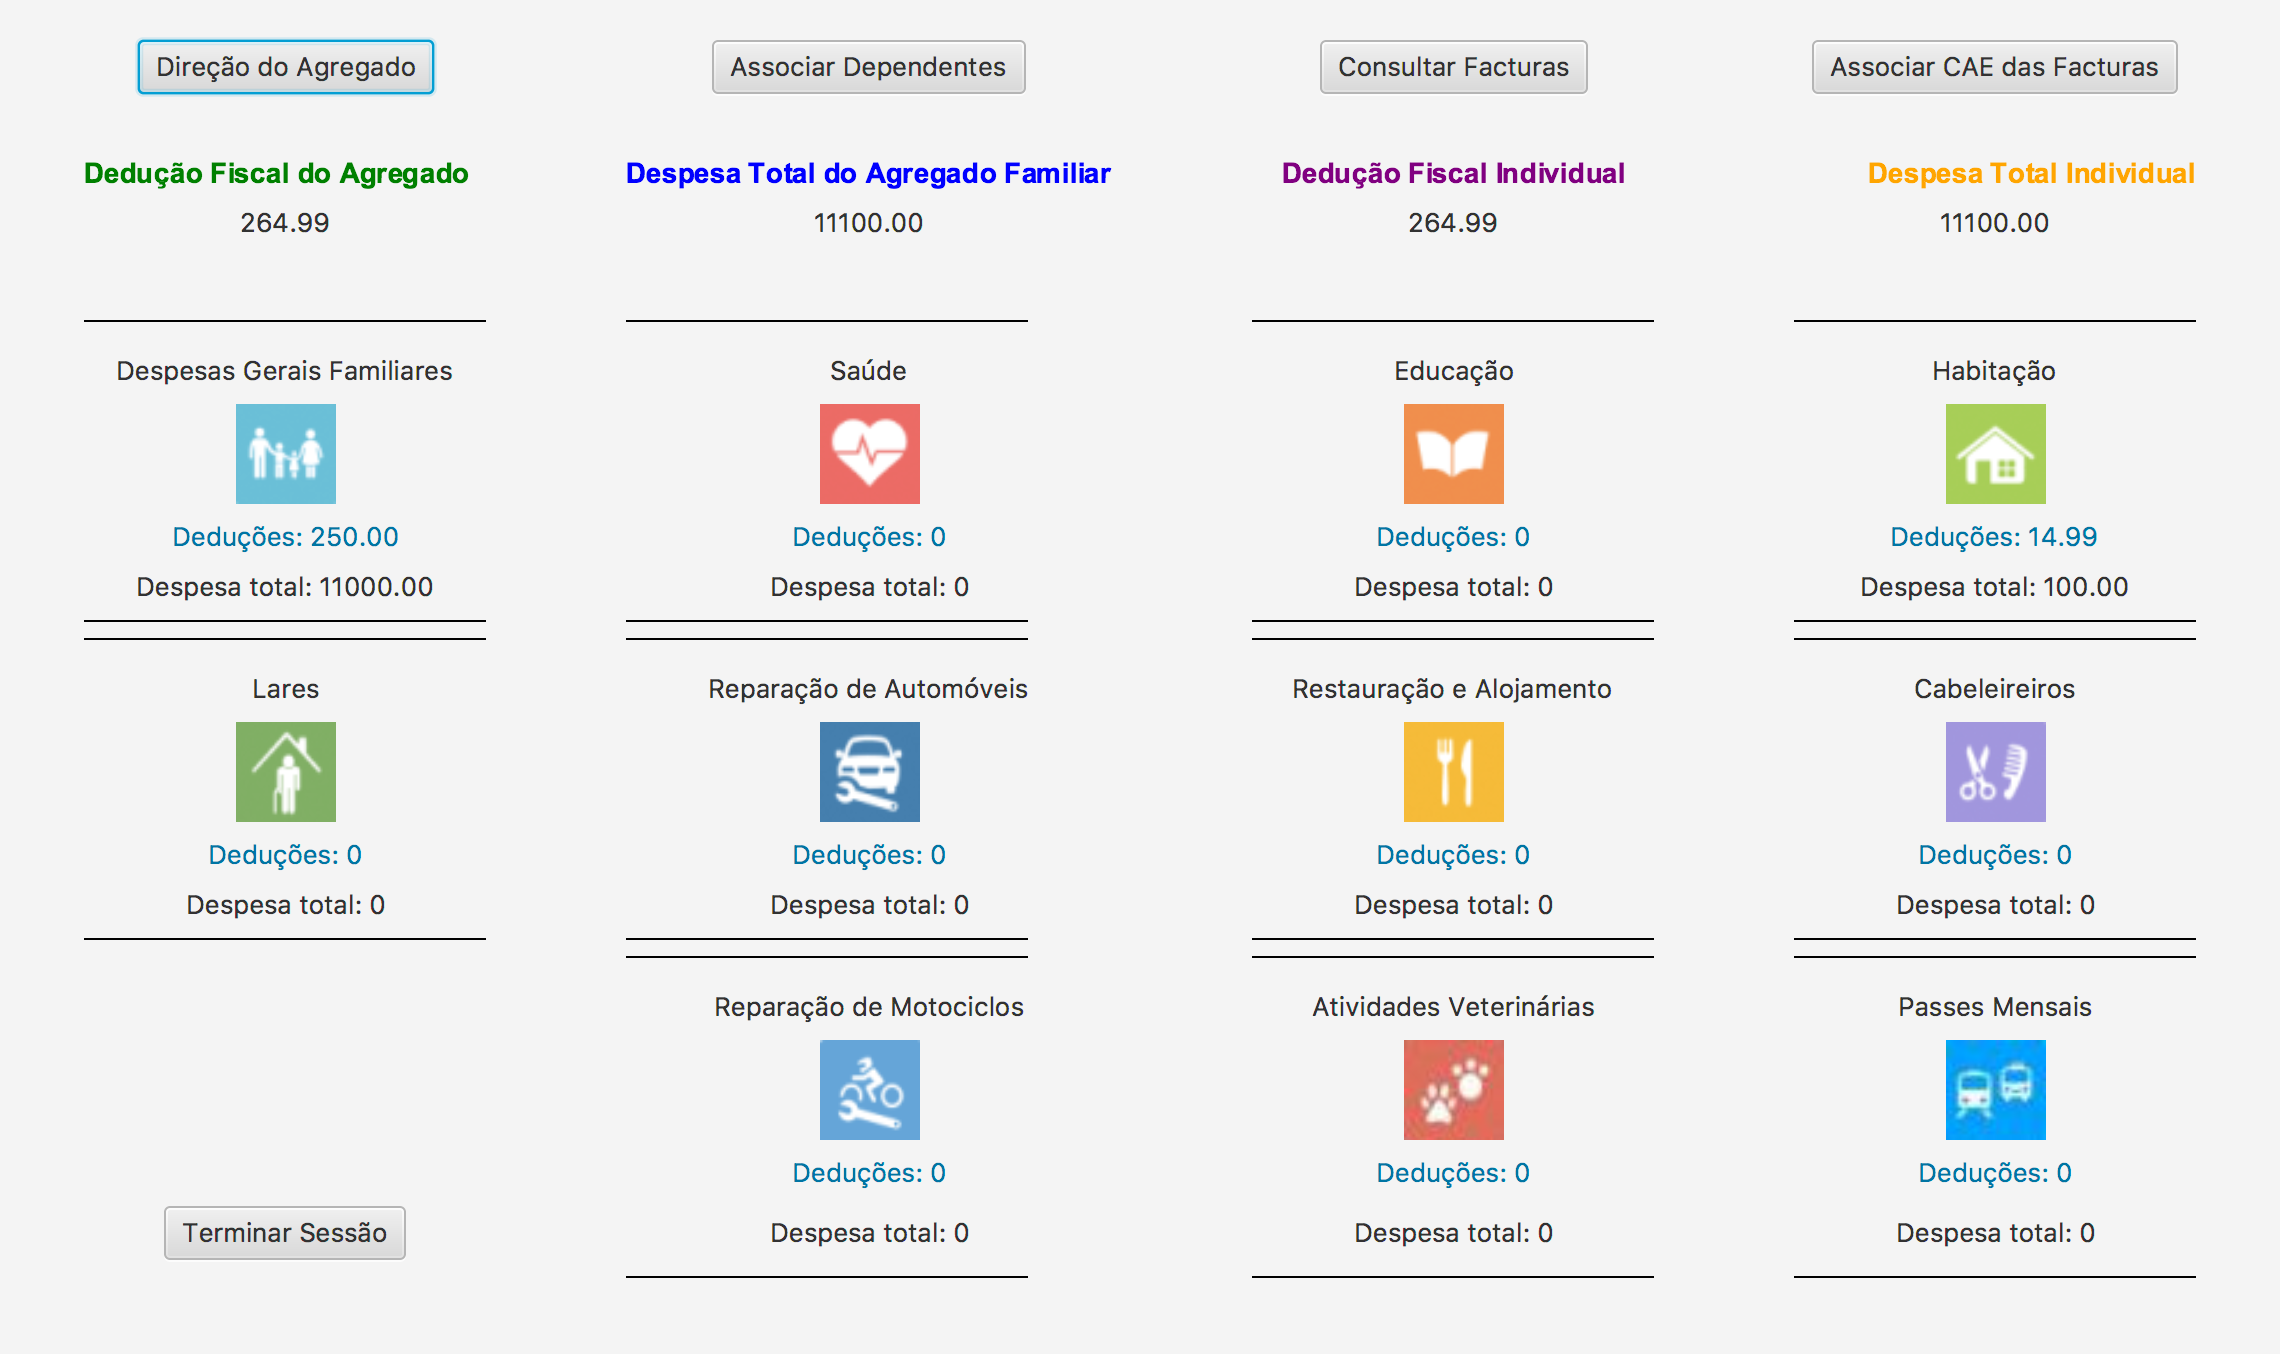
\includegraphics[scale=0.35]{imgs/dashboardindividual.png}
\caption{Dashboard Contribuinte Individual.}
\label{img:dashboardindividual}
\end{figure}


E caso tenha sido um Contribuinte Coletivo aparece a seguinte dashboard:
\begin{figure}[H]
\centering
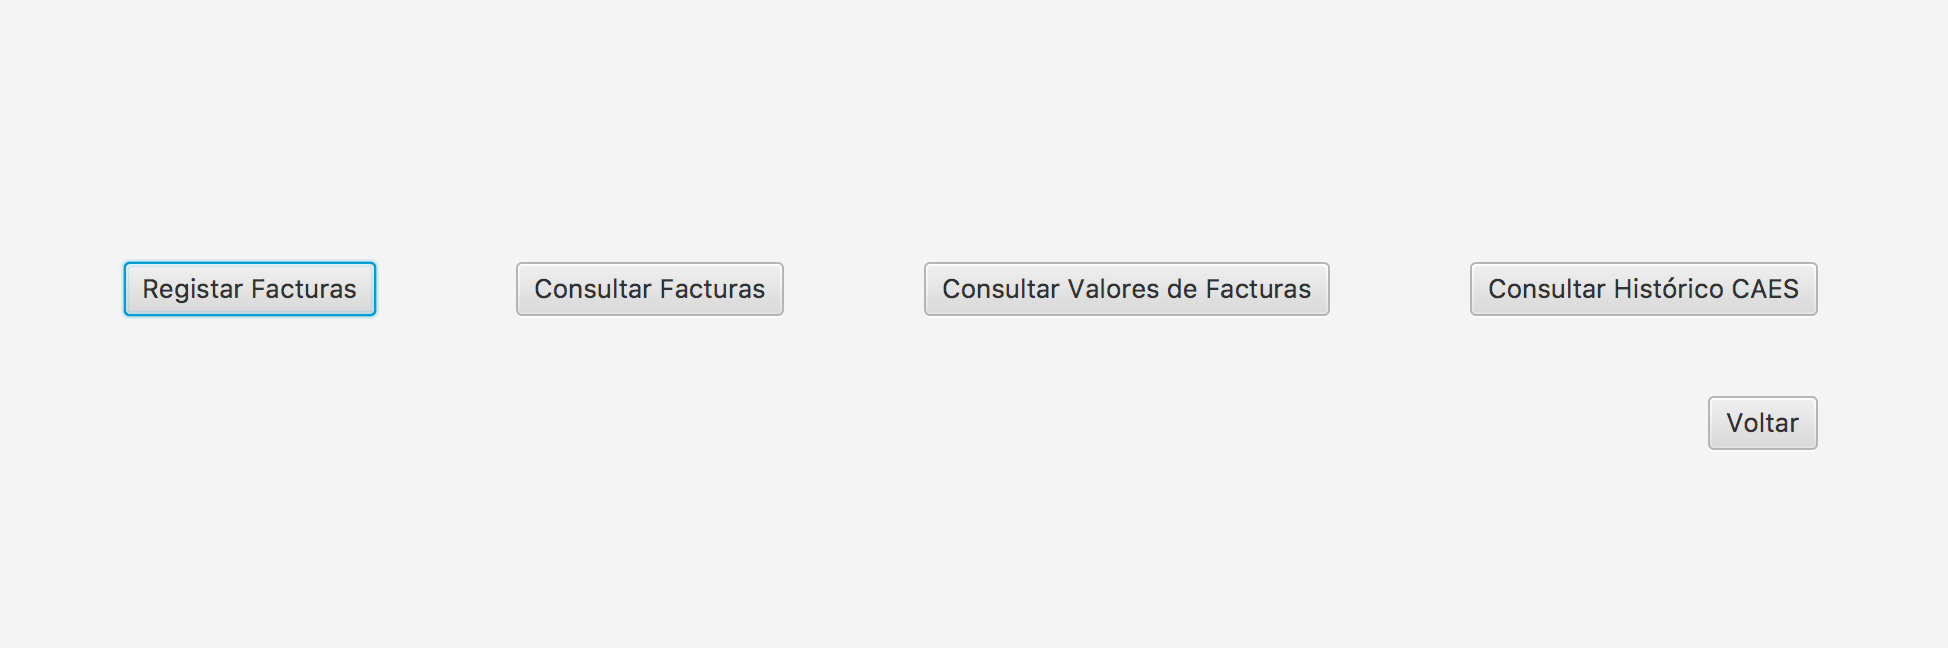
\includegraphics[scale=0.40]{imgs/dashboardcoletivo.png}
\caption{Dashboard do Contribuinte Coletivo.}
\label{img:dashboardcoletivo}
\end{figure}


\begin{figure}[H]
\centering
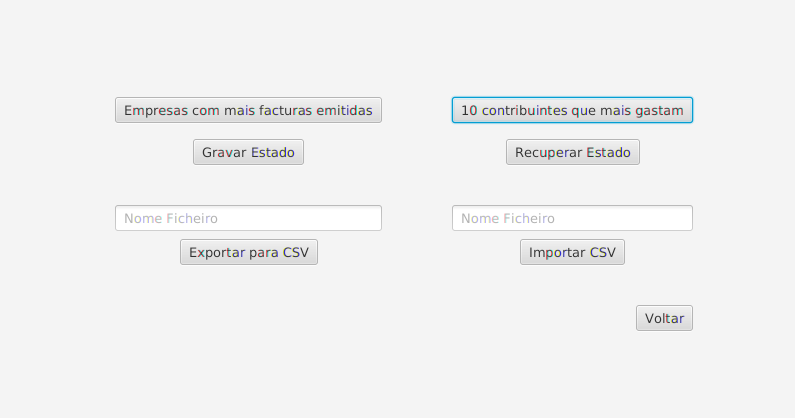
\includegraphics[scale=0.40]{imgs/dashboardadmin.png}
\caption{Dashboard do Administrador.}
\label{img:dashboardadmin}
\end{figure}

É a partir destas dashboards que os atores do sistema poderão realizar
as operações que mais lhes convêm, uma vez que é aqui que as funcionalidades do
nosso programa estão incutidas.



\subsection{Criar Faturas}
\label{sec:criarfaturas}

\item \textbf{Criar faturas associadas a despesas feitas por um contribuinte individual.
São as empresas que alimentam esta informação no sistema.}

Os contribuintes coletivos podem criar faturas em nome de contribuintes individuais.
Para tal, deverão selecionar o respetivo botão de ``Registar Facturas'' na sua dashboard,
onde são reencaminhados para o seguinte formulário:

\begin{figure}[H]
\centering
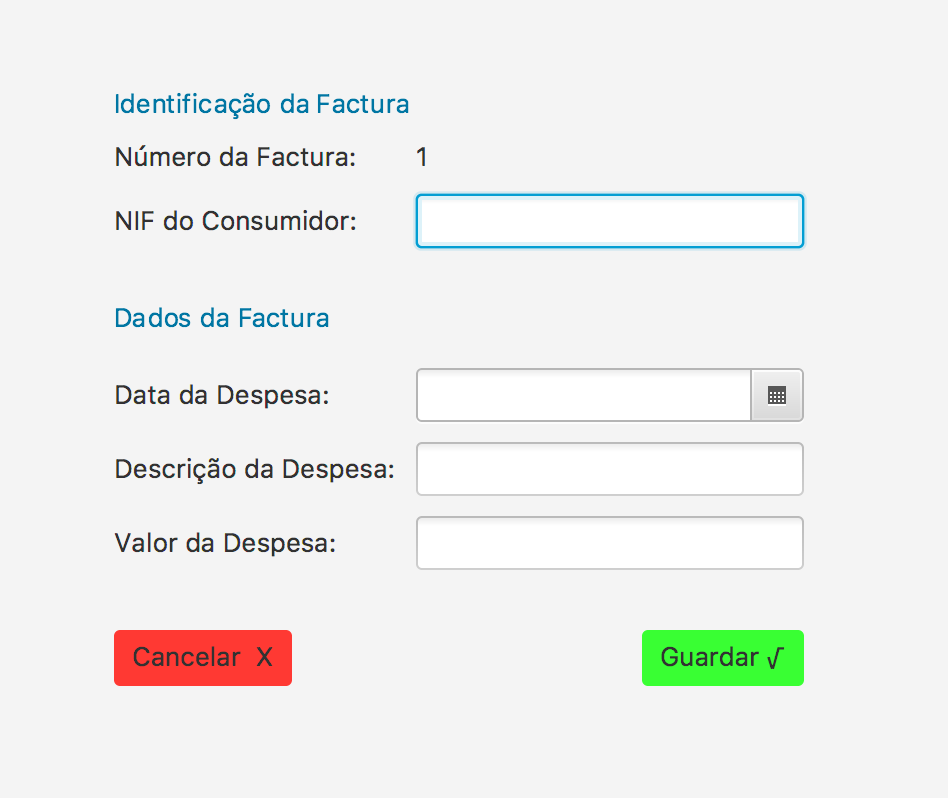
\includegraphics[scale=0.40]{imgs/registarfatura.png}
\caption{Registar uma Fatura.}
\label{img:registarfatura}
\end{figure}

Deverão preencher todos os campos disponíveis. Existem outros campos que são automaticamente
preenchidos tendo em conta alguns aspetos do contribuinte coletivo, como é o caso
do nome da empresa emitente, o número da fatura, a natureza económica da fatura
(que é já definida se o contribuinte coletivo só tiver inserido numa atividade
económica, caso contrário, fica a 0 (Sem Atividade)) e o histórico dos caes da
fatura (que caso a empresa esteja emergente em mais do um setor de atividade
começa por ser 0, caso contrário, o histórico é e sempre será vazio).

\vspace{0.1cm}

Assim, é criada a fatura através do seu construtor parametrizado e respetivamente
adicionada a cada um dos dois contribuintes relacionados com a mesma:

\begin{figure}[H]
\centering
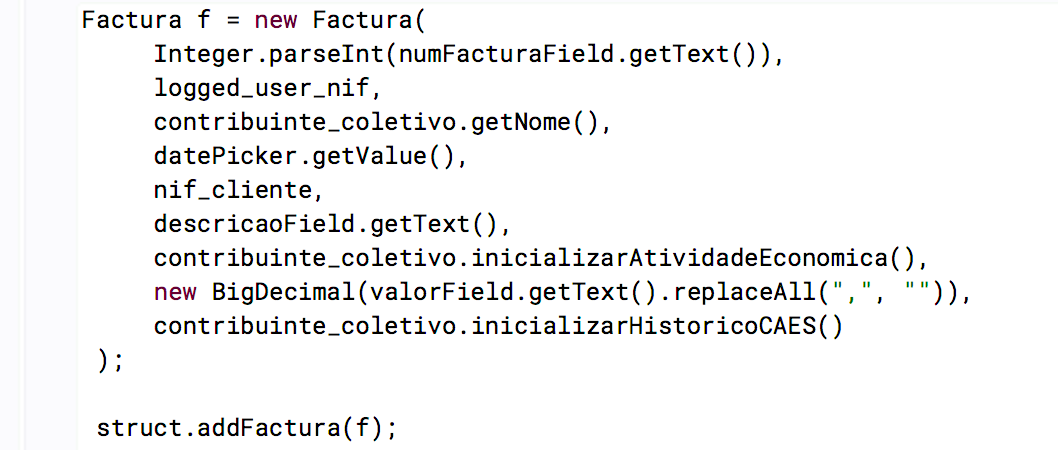
\includegraphics[scale=0.40]{imgs/registarfatura_func.png}
\caption{Registar uma Fatura (métodos).}
\label{img:registarfatura_func}
\end{figure}

O método \textsf{addFatura}, "chama" outros dois métodos, que adicionam as faturas a cada um
dos objetos (Contribuinte Individual e Contribuinte Coletivo):

\begin{figure}[H]
\centering
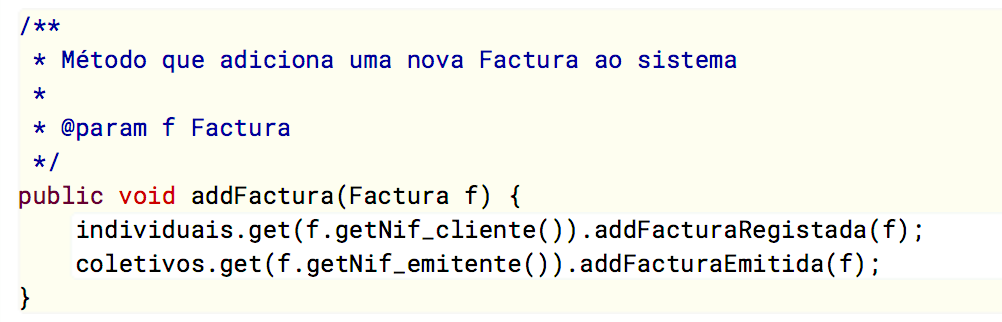
\includegraphics[scale=0.40]{imgs/addFatura.png}
\caption{Adicionar uma Fatura (método geral).}
\label{img:addFatura}
\end{figure}


O método que adiciona a fatura ao Contribuinte Individual é a apresentada em seguida,
e o raciocínio utilizado consiste em inicialmente determinar qual é o código do setor
de atividade da fatura (0 se não tiver atividade definida) para posteriormente adiciona-la
ao ``map'' das faturas do Contribuinte Individual, onde a chave é o código do setor.

\begin{figure}[H]
\centering
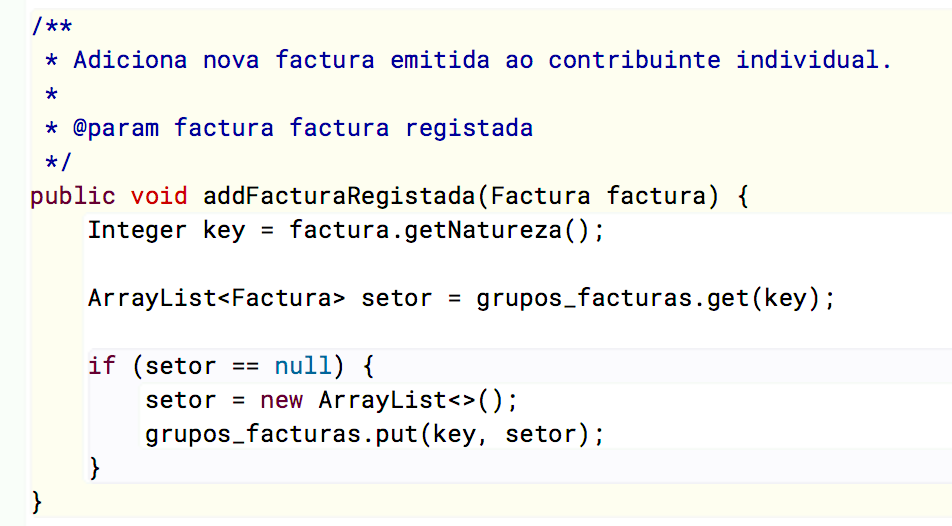
\includegraphics[scale=0.40]{imgs/addFacturaRegistada.png}
\caption{Adicionar uma Fatura ao Contribuinte Individual.}
\label{img:addFacturaRegistada}
\end{figure}


E para adicionar a fatura ao Contribuinte Coletivo basta simplesmente
adicionar a fatura à lista das faturas emitidas:

\begin{figure}[H]
\centering
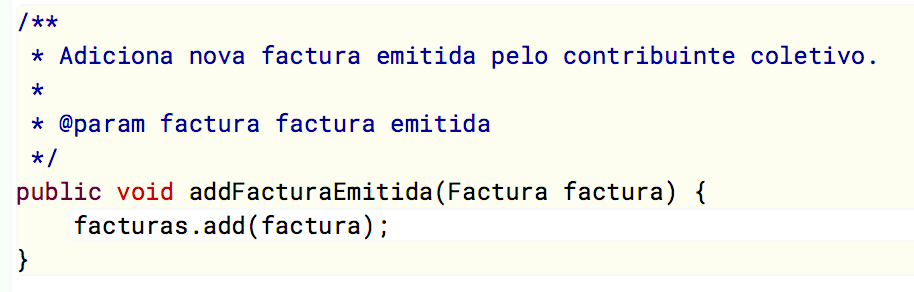
\includegraphics[scale=0.40]{imgs/addFacturaEmitida.png}
\caption{Adicionar uma Fatura ao Contribuinte Coletivo.}
\label{img:addFacturaEmitida}
\end{figure}


\subsection{Verificar Despesas e Montantes Dedução Fiscal}
\label{sec:despesasemontantes}

\item \textbf{Verificar, por parte do contribuinte individual, as despesas que foram emitidas
em seu nome e verificar o montante de dedução fiscal acumulado, por si e pelo agregado familiar.}

Tendo em conta que uma das principais funções do programa é calcular as
deduções a que os contribuintes têm direito, implementamos métodos que nos permitem
não só calcular as deduções do contribuinte individual e despesas por si suportadas, mas
também verificar o montante da despesa suportada pelo seu agregado, bem como verificar
o valor total das deduções obtidas por todos os elementos do agregado
familiar.
De facto, conforme podemos observar na parte superior do painel informativo
representado na Figura~\ref{img:dashboardindividual}, estão contabilizadas as deduções
fiscais e a despesa total dos elementos do seu agregado, bem como as deduções e as
despesas efetuadas pelo contribuinte individual.
Ademais, definimos ainda métodos que nos permitem também discriminar o montante
das deduções e das despesas efetuadas por um indivíduo em cada um dos setores de atividade,
o que é também possível verificar através do referido painel.
Assim, sempre que é emitida uma fatura a um determinado contribuinte os valores inscritos
no seu painel informativo são atualizados.



\subsection{Associar CAE}
\label{sec:associarcae}

\item \textbf{Associar classificação de atividade económica a um documento de despesa.}

Outros dos objetivos do trabalho prático é associar uma classificação de atividade
económica a um documento de despesa. Assim como no e-fatura, quando a empresa que emite
uma fatura está inserida em mais do que um setor de atividade o CAE da fatura fica
indefinido (no nosso caso fica com código 0, que corresponde a Sem Atividade).

Como forma de colmatar este problema, na sua dashboard, o contribuinte individual
tem a opção \textbf{Associar CAE das Faturas}, como se pode ver na
Figura~\ref{img:dashboardindividual}, onde se encontram impressas todas as faturas
do contribuinte individual que têm natureza 0 (corresponde ao ArrayList
com chave 0 do ``map'').

Deste modo, após selecionar essa opção o utilizador encontra uma tabela com todas
as faturas sem CAE definido, onde o mesmo poderá selecionar o CAE que se adequa
ao serviço que usufruiu. No nosso caso, optamos por só imprimir os CAEs disponíveis
pelo contribuinte coletivo que emitiu a fatura, mas caso imprimissemos todos
o programa apenas aceitaria o CAE se a empresa emitente o tivesse.

\begin{figure}[H]
\centering
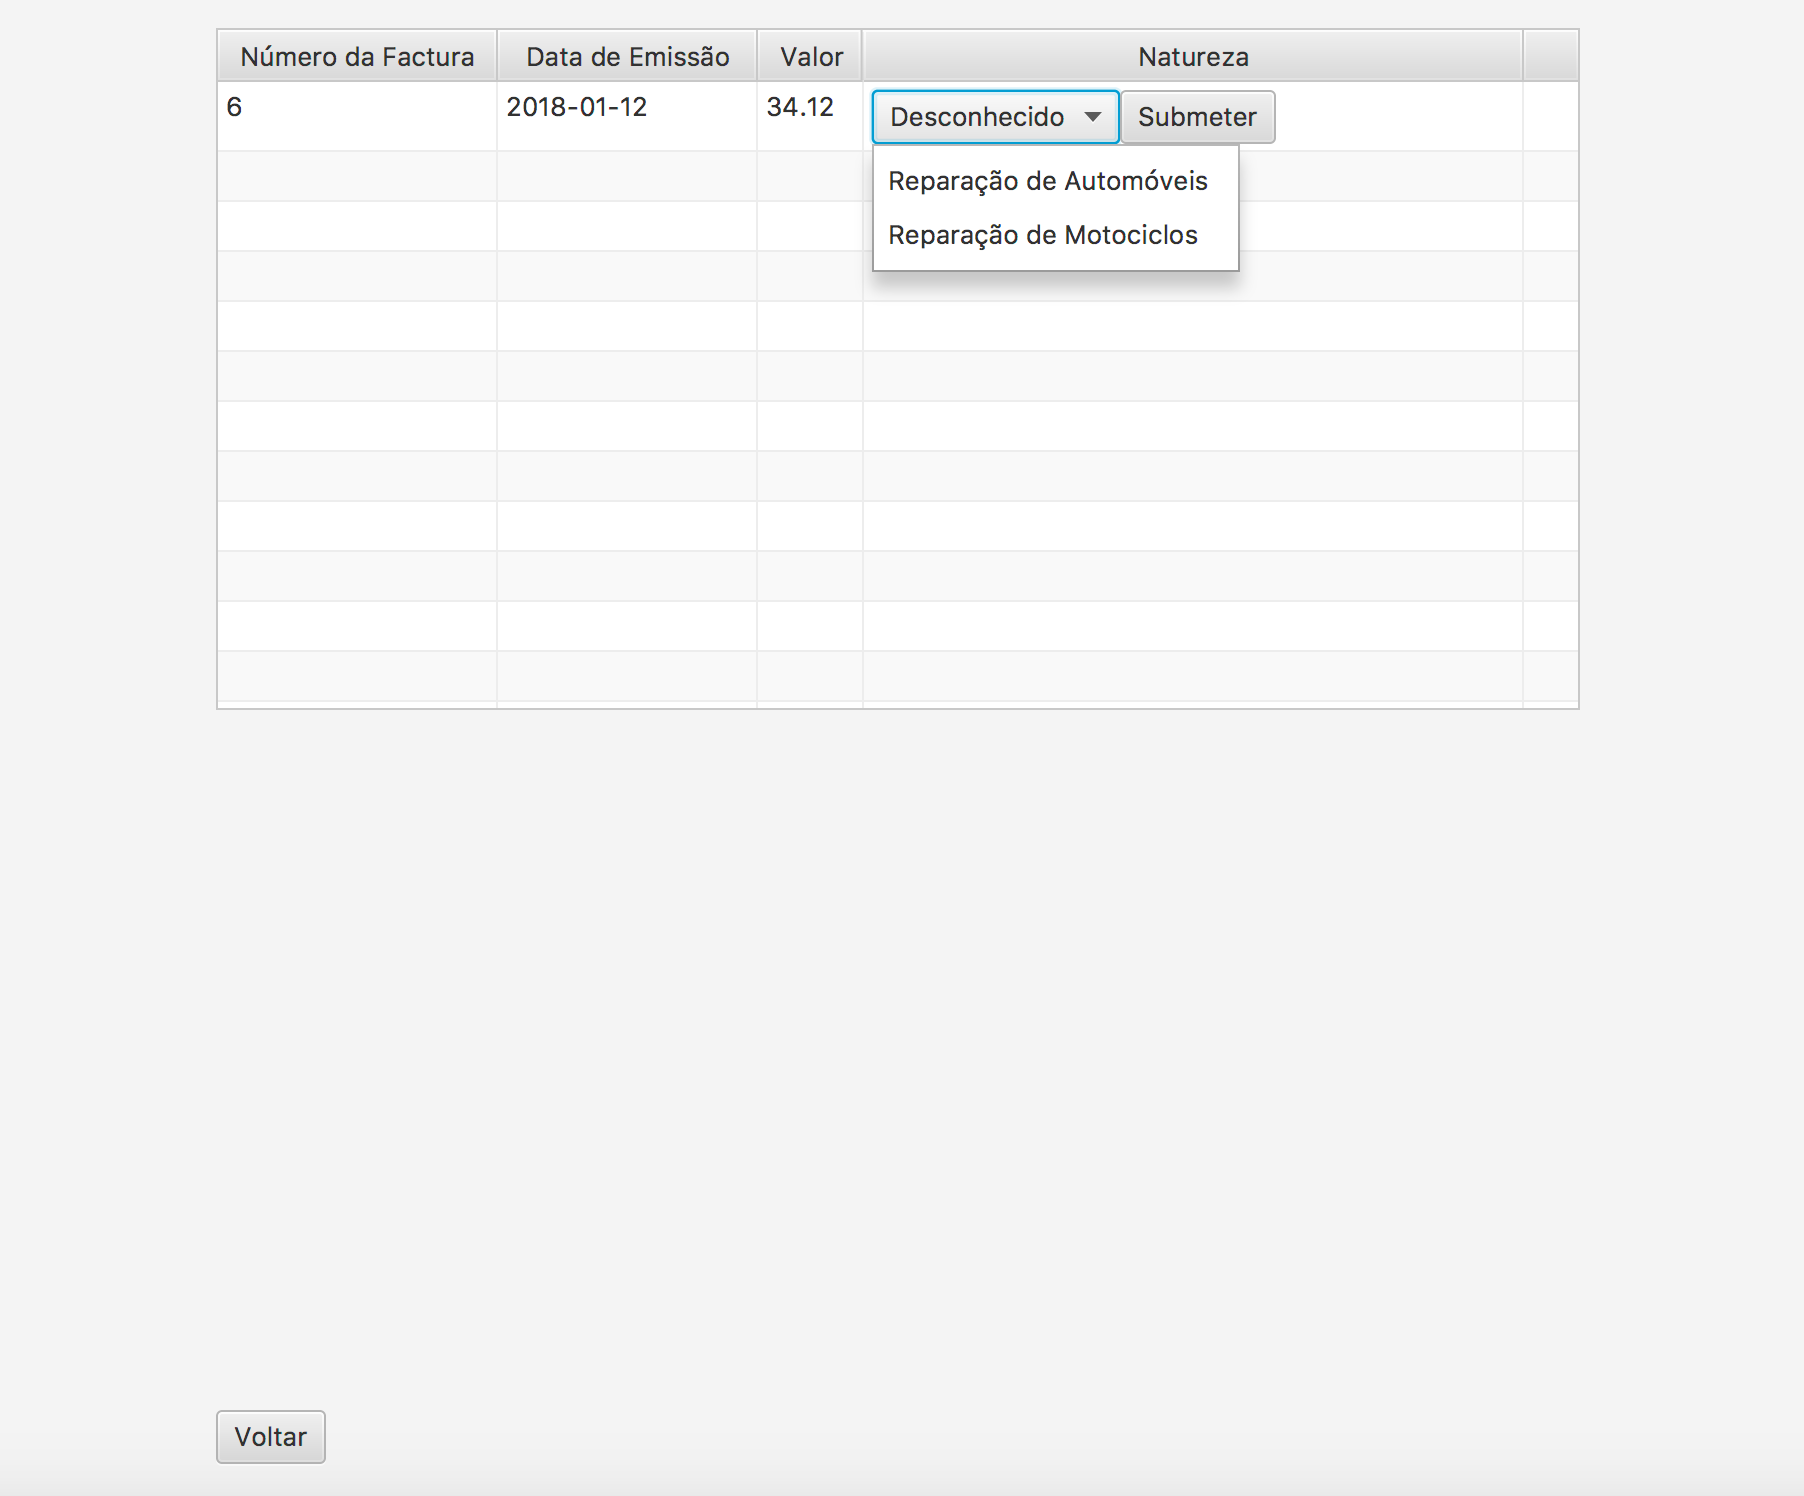
\includegraphics[scale=0.35]{imgs/associarcaetable.png}
\caption{Associar CAE das Faturas (Tabela).}
\label{img:associarcaetable}
\end{figure}

Após selecionar o CAE e carregar em \textbf{Submeter}, no nosso programa
é chamado o método \textsf{setCAEFactura} (Figura~\ref{img:setCAEFactura}),
e passados como parâmetros o apontador da fatura, o NIF do contribuinte individual
que está loggado e o número do código correspondente ao setor de atividade escolhido
pelo contribuinte individual.

Em seguida, se o contribuinte coletivo possuir esse determinado CAE
(o que no nosso caso é garantido devido à disposição da interface gráfica)
é chamado o método \textsf{setCAE} (Figura~\ref{img:setCAE}),
um método do Contribuinte Individual.

Este método tem a responsabilidade de eliminar a fatura do ArrayList de faturas
com o código 0 do ``map'' e de a adicionar ao ArrayList com o código a que a fatura
agora pertence. Para além disso, como é pedido no requisito da Secção~\ref{sec:mudarcae},
a fatura tem associada a si um histórico dos CAEs que já possuiu, e, assim sendo,
este método adiciona a esse histórico o novo CAE da fatura (este método e em particular
a funcionalidade do histórico vai ser novamente
explicada na Secção~\ref{sec:mudarcae}).



\begin{figure}[H]
\centering
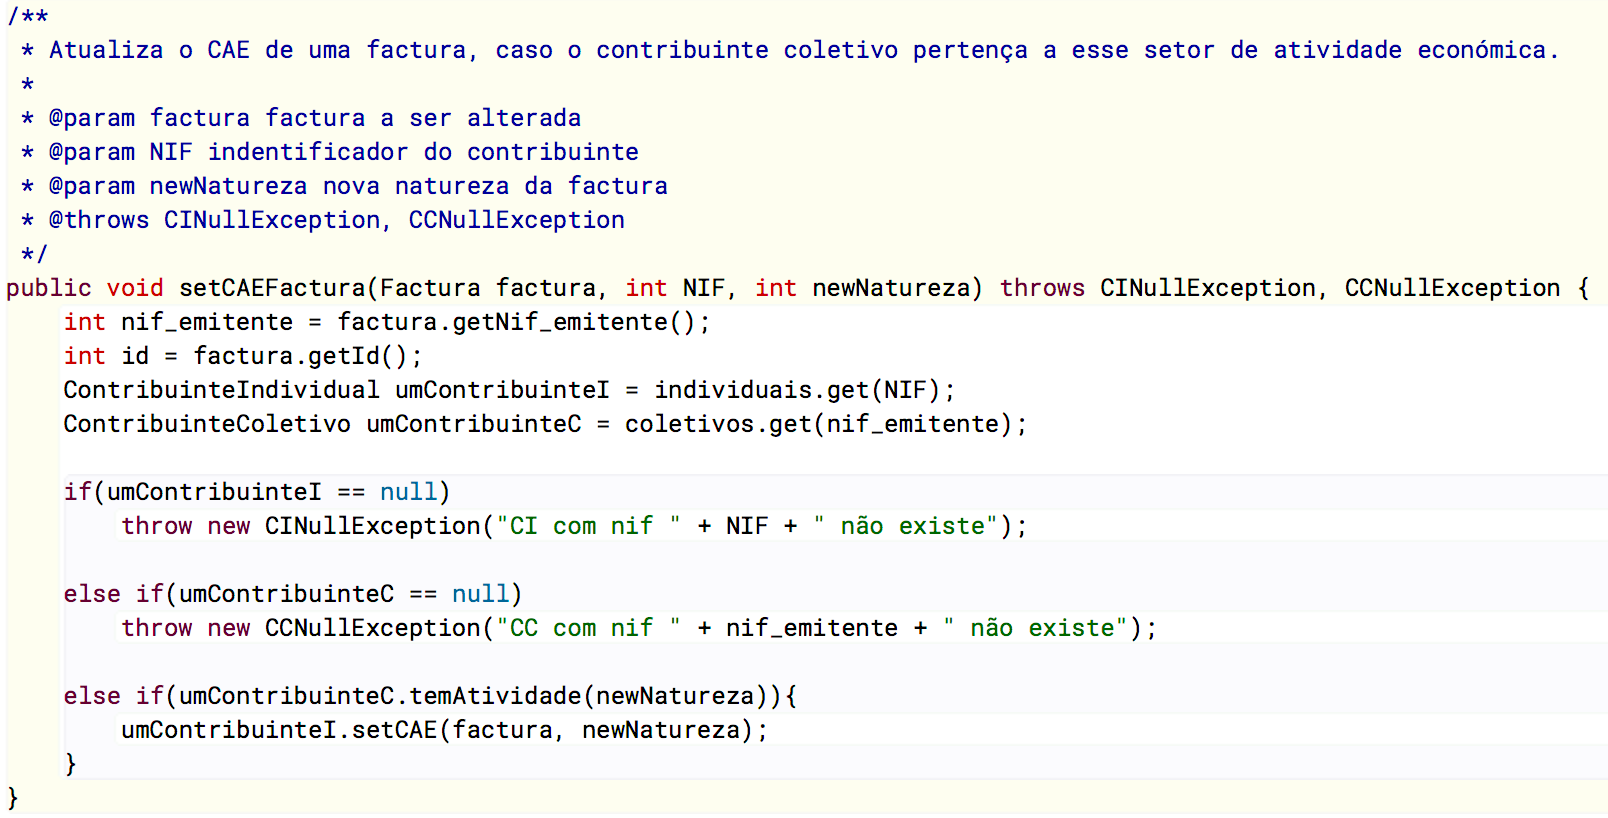
\includegraphics[scale=0.35]{imgs/setCAEFactura.png}
\caption{Associar CAE das Faturas- Método da classe JavaFactura.}
\label{img:setCAEFactura}
\end{figure}

\begin{figure}[H]
\centering
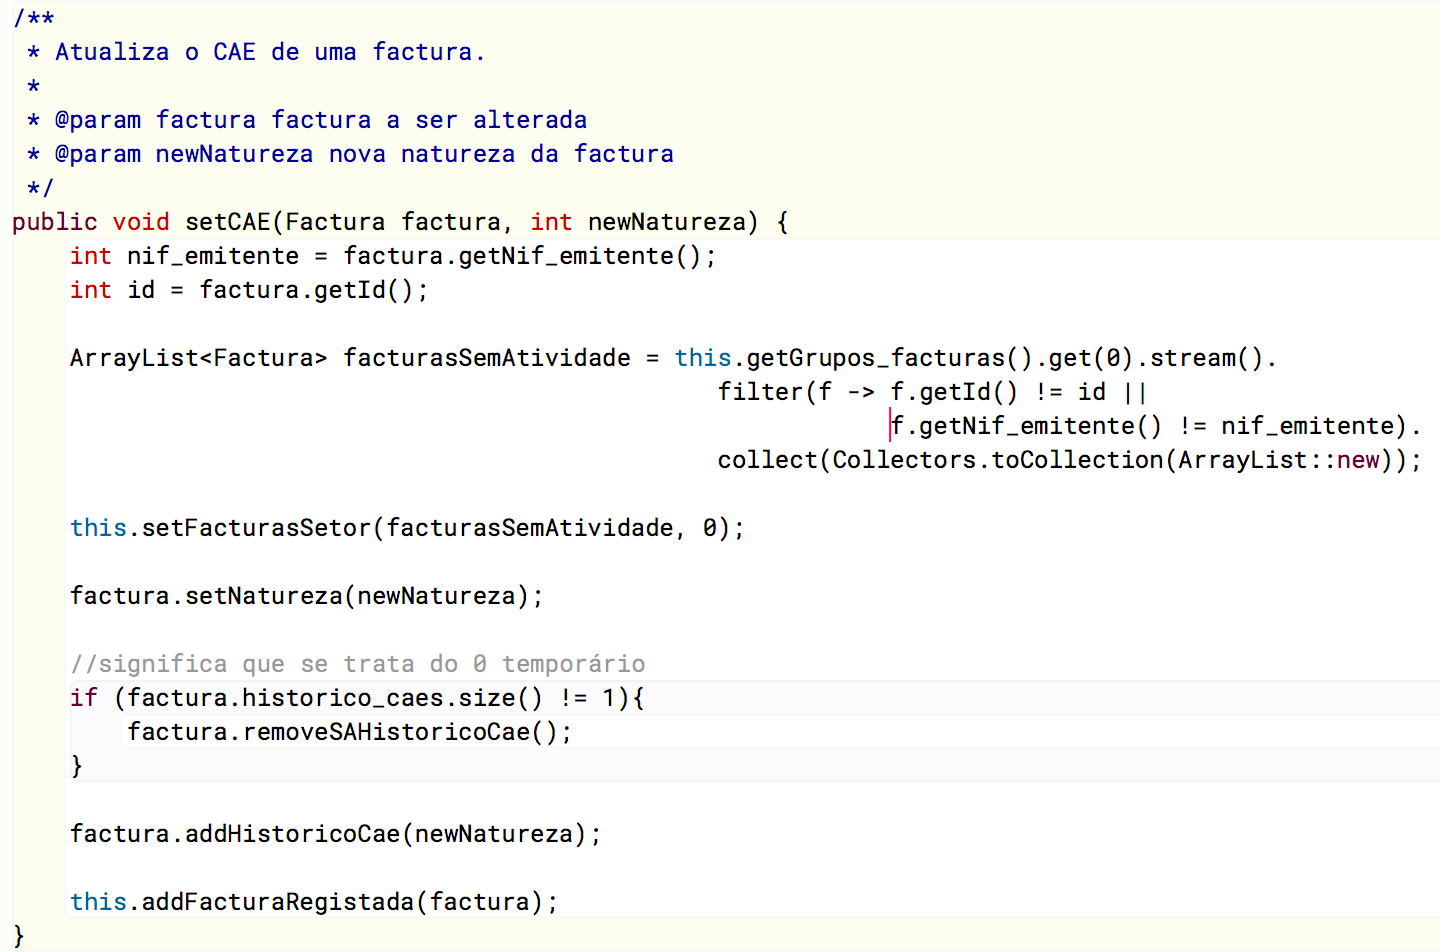
\includegraphics[scale=0.35]{imgs/setCAE.png}
\caption{Associar CAE das Faturas- Método da classe ContribuinteIndividual.}
\label{img:setCAE}
\end{figure}


\subsection{Mudar CAE}
\label{sec:mudarcae}

\item \textbf{Corrigir a classificação de atividade económica de um documento de despesa.
Esta alteração deve deixar registo para ser depois rastreada.}

Na aba \textbf{Consultar Facturas} (visível na dashboard do Contribuinte Individual,
Figura~\ref{img:dashboardindividual}) o contribuinte individual tem a opção de visualizar
todas as faturas emitidas com o seu NIF.

Nesse separador, ilustrado na Figura~\ref{img:consultafaturas}, o contribuinte tem
a hipótese de alterar o CAE de uma fatura com um CAE já definido. É de referir que
as faturas emitidas por uma empresa que exerce em apenas um setor económico
não oferecem essa hipótese de mudança de CAE. Na nossa interface gráfica, para
essas faturas com CAE "obrigatório" não é sequer
impressa a opção de \textbf{Alterar CAE}, mas caso fosse, se o utilizador tentasse
alterar o CAE o programa não deixaria.

\begin{figure}[H]
\centering
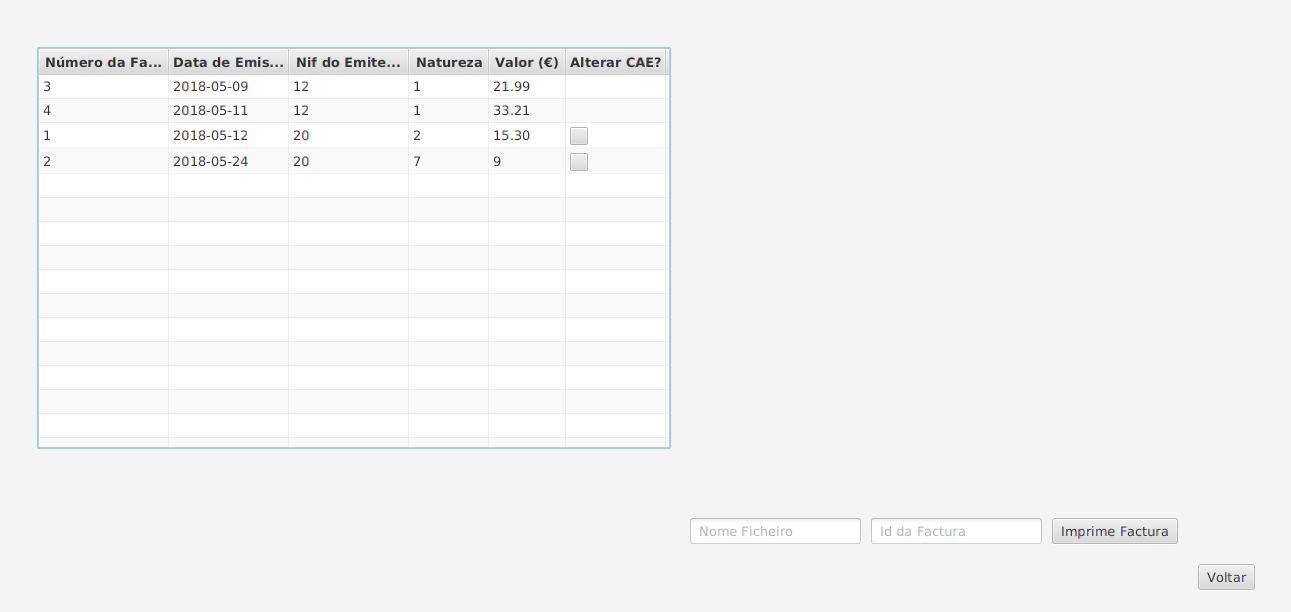
\includegraphics[scale=0.35]{imgs/consultafaturas.png}
\caption{Consulta Faturas (tabela).}
\label{img:consultafaturas}
\end{figure}


Quando pressionado o botão da coluna \textbf{Alterar CAE} a natureza da fatura passa a 0
uma vez que é invocado o método \textsf{eliminarCaeFatura} (classe \textsf{JavaFactura},
Figura~\ref{img:eliminarCaeFatura}), que
por sua vez chama o método \textsf{eliminaCAE} (classe \textsf{Contribuinte Individual},
Figura~\ref{img:eliminaCAE}).

Estes métodos são as responsáveis por averiguar se o contribuinte coletivo emissor da fatura
está inserido em mais do que um setor (é chamado o método \textsf{podemAlterarCAEfaturas},
classe \textsf{Contribuinte Coletivo}) e por alterar efetivamente o CAE da fatura, respetivamente.

O método que altera efetivamente o CAE da fatura (Figura~\ref{img:eliminaCAE})
é a responsável por eliminar a fatura
do ArrayList correspondente ao código da natureza antiga do ``map'' e inseri-la no ArrayList
correspondente ao código 0, com a fatura agora também com natureza 0.

\begin{figure}[H]
\centering
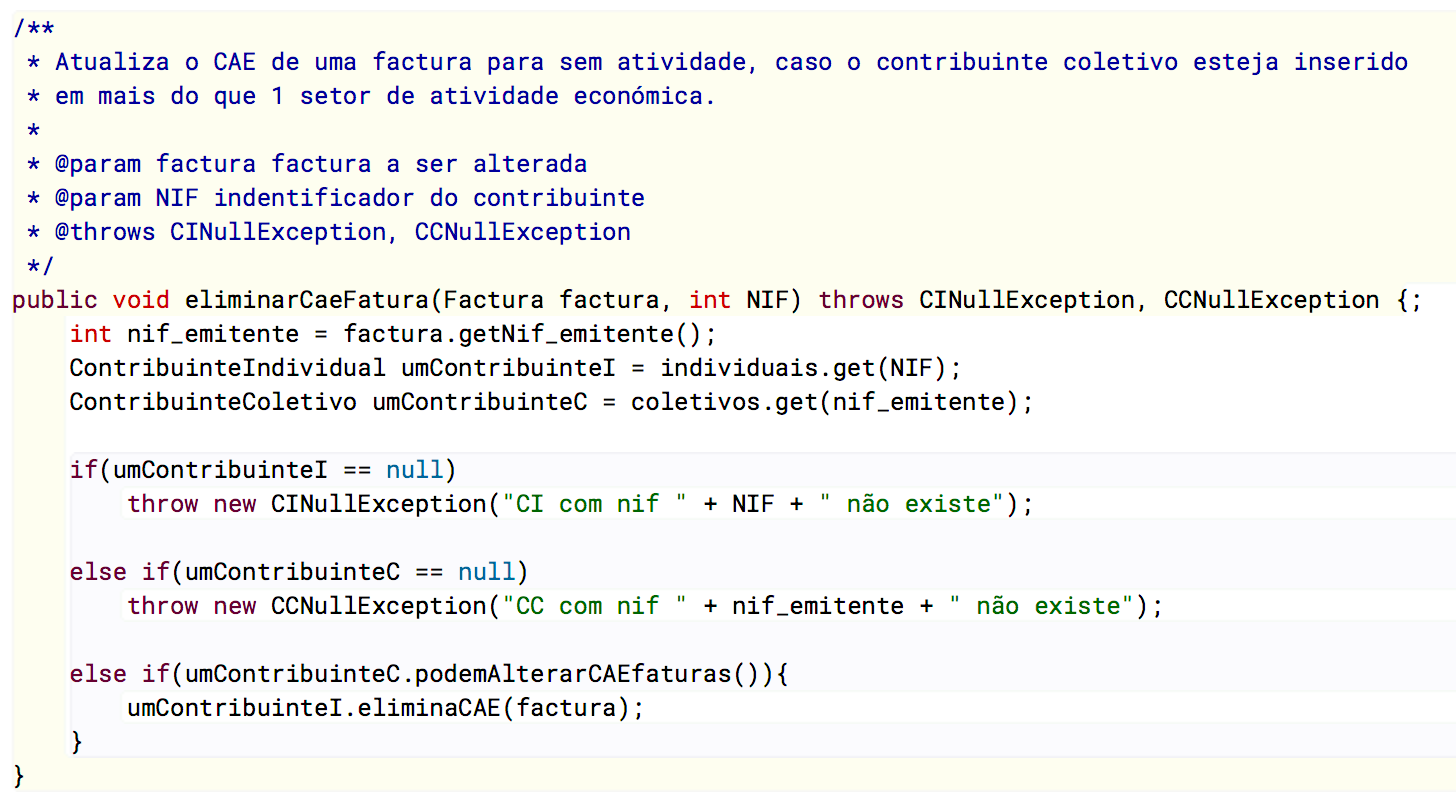
\includegraphics[scale=0.35]{imgs/eliminarCaeFatura.png}
\caption{Eliminar o CAE da Fatura (método JavaFactura).}
\label{img:eliminarCaeFatura}
\end{figure}

\begin{figure}[H]
\centering
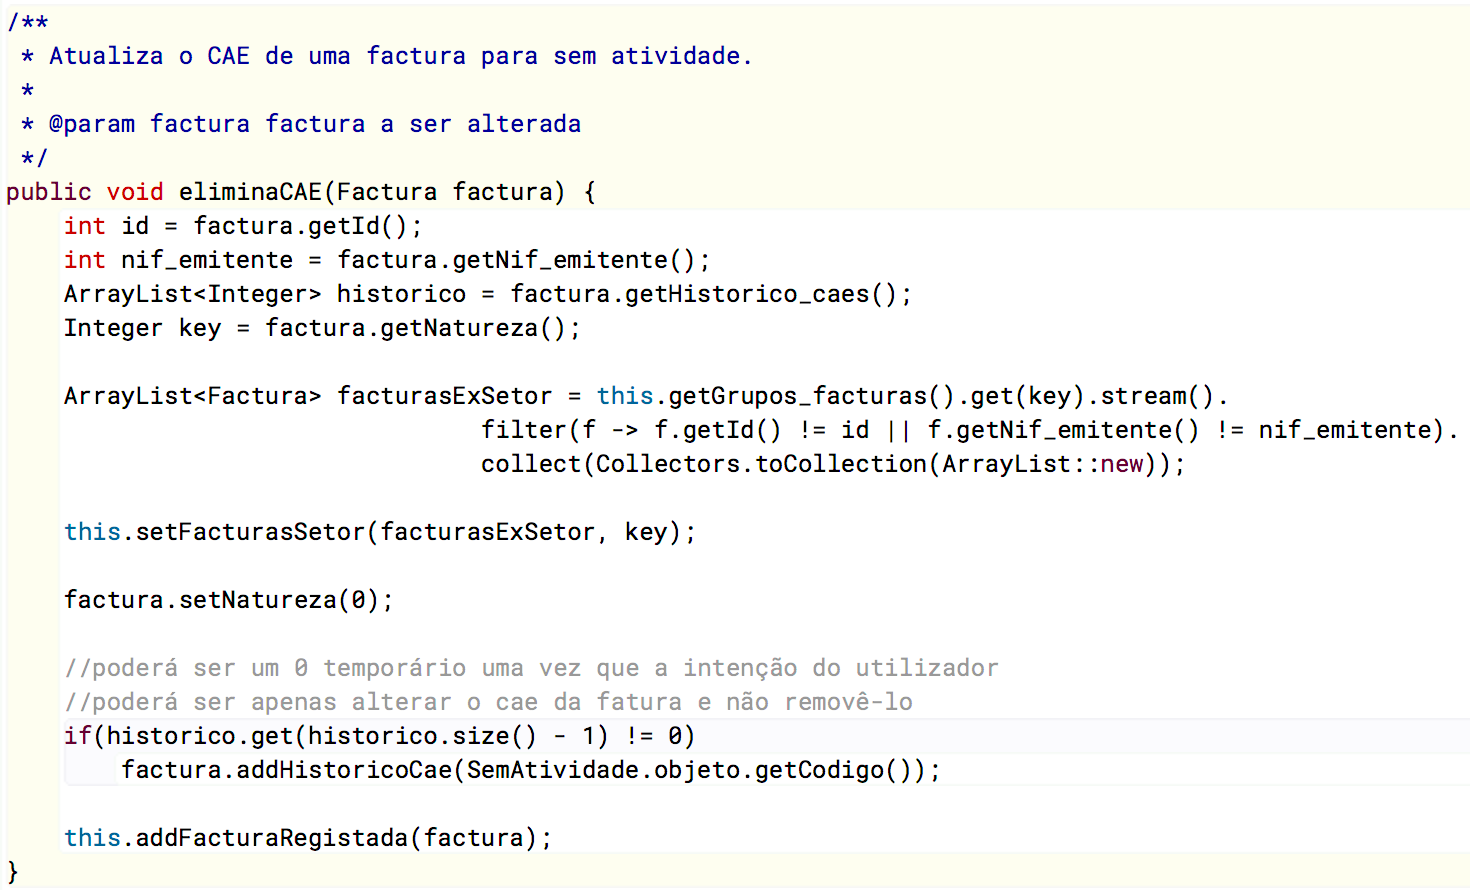
\includegraphics[scale=0.35]{imgs/eliminaCAE.png}
\caption{Eliminar o CAE da Fatura (método ContribuinteIndividual).}
\label{img:eliminaCAE}
\end{figure}

Para além disso, este método é também responsável por adicionar um 0 ao histórico dos CAEs, caso
não haja já lá um 0 (quando a fatura é criada e não possui à partida CAE definido o seu
histórico começa com um 0), ou seja, a última posição do ArrayList histórico será necessariamente
um 0. Este 0 é importante para que a empresa possa saber que, de momento, aquela fatura não tem
um CAE escolhido pelo contribuinte individual.

Assim, uma vez que a fatura pertence agora ao ArrayList de faturas sem CAE definido, quando
o utilizador pressionar novamente o botão de \textbf{Associar CAE das Faturas}, presente
na sua dashboard individual, essa fatura
estará impressa nessa tabela e o utilizador poderá escolher de novo qual o CAE que melhor se
adequa àquela fatura.

Deste modo, depois de eliminar o CAE atual da fatura, é adicionado ao ArrayList histórico o código 0.
Se a intenção do utilizador for mesmo alterar o CAE da fatura para um outro de imediato esse 0 foi
apenas um código temporário, pelo que o método \textsf{setCAE}, (Figura~\ref{img:setCAE},
mencionado na Secção~\ref{sec:associarcae}), tem em atenção esse 0
e elimina-o do histórico. O único 0 do histórico que se manterá é o 0 inicial do ArrayList,
que representa que a empresa que emitiu a fatura atua em mais do que um setor de atividade económica,
o que dá para concluir que o CAE da fatura é o CAE entendido pelo utilizador.

O contribuinte coletivo tem a oportunidade de consultar esse histórico clicando no botão
\textbf{Consultar Histórico CAES}, presente na sua dashboard (Figura~\ref{img:dashboardcoletivo}).
Nesse separador é apresentada a tabela presente na Figura~\ref{img:historicocaes}, que basicamente imprime
para cada fatura emitida pela empresa a sua variável de instância historico\_caes.

\begin{figure}[H]
\centering
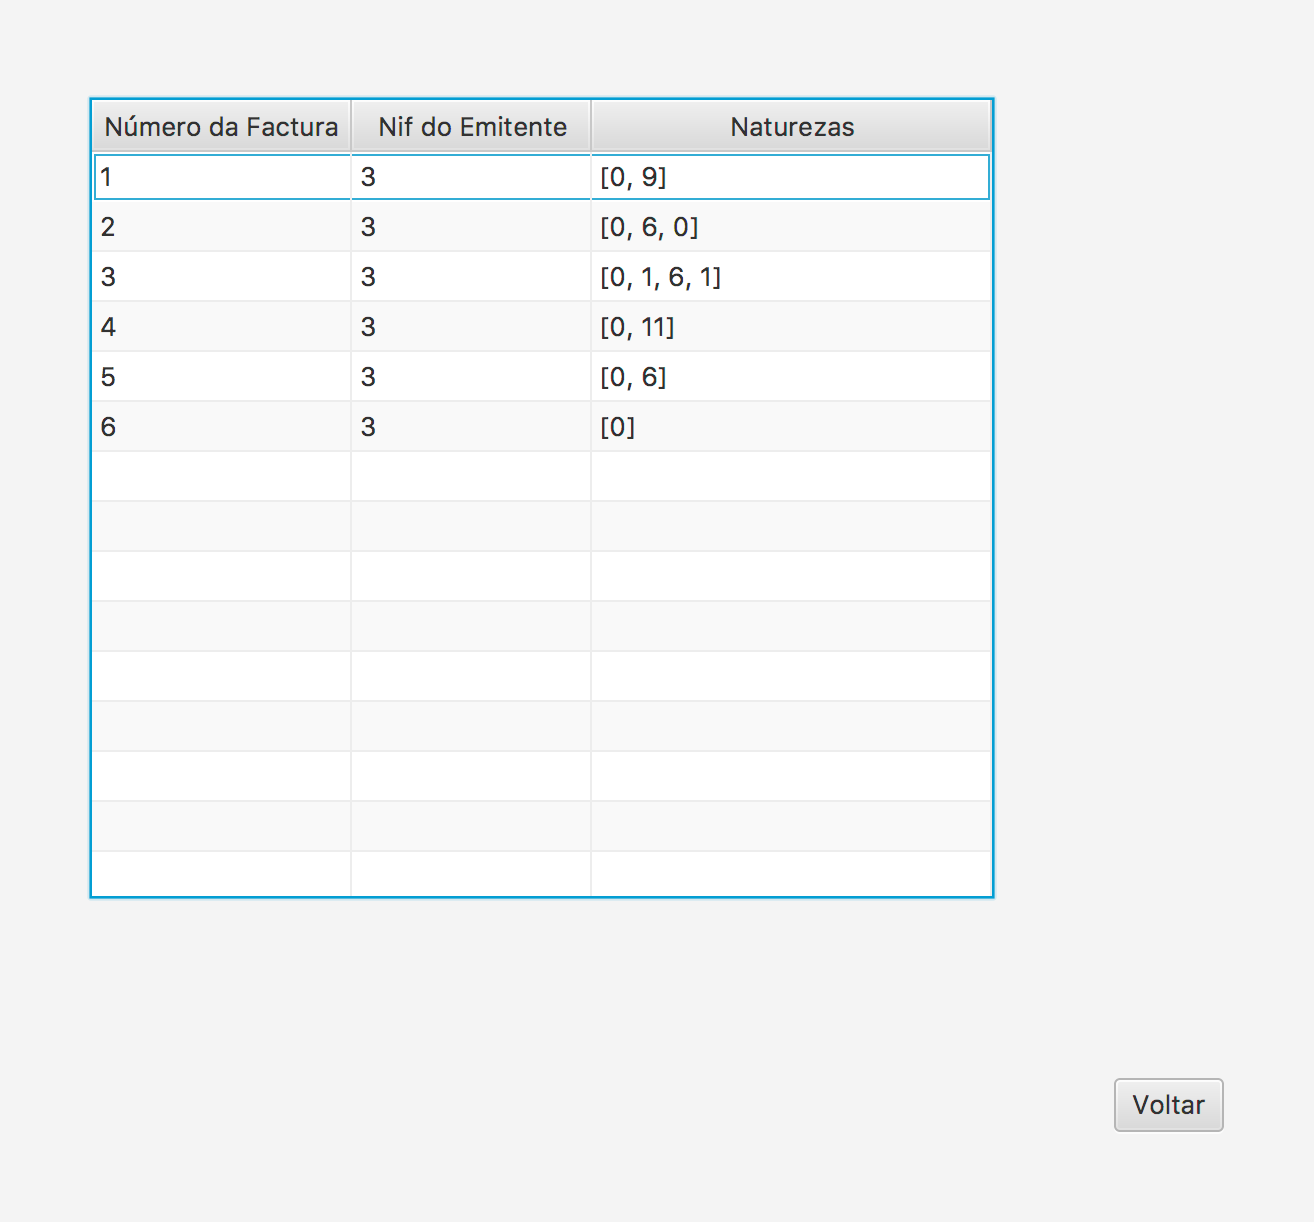
\includegraphics[scale=0.35]{imgs/historicocaes.png}
\caption{Histórico dos CAEs das Faturas (Contribuinte Coletivo).}
\label{img:historicocaes}
\end{figure}



\subsection{Listagem das Faturas Empresas (Data e Valor)}
\label{sec:listagemfempresas}

\item \textbf{Obter a listagem das faturas de uma determinada empresa, ordenada por data
de emissão ou por valor.}

O contribuinte coletivo tem a opção de obter a listagem das suas faturas
ordenadas por data de emissão. Para tal, na sua dashboard
(Figura~\ref{img:dashboardcoletivo}),
após pressionar o botão \textbf{Consultar Facturas}, aparecerá a dashboard representada na
Figura~\ref{img:consultarFaturas}, onde estão visíveis todas as faturas emitidas por si.
Para as ordenar por data, o contribuinte terá que carregar no botão \textbf{Ordenar todas por Data}.

\begin{figure}[H]
\centering
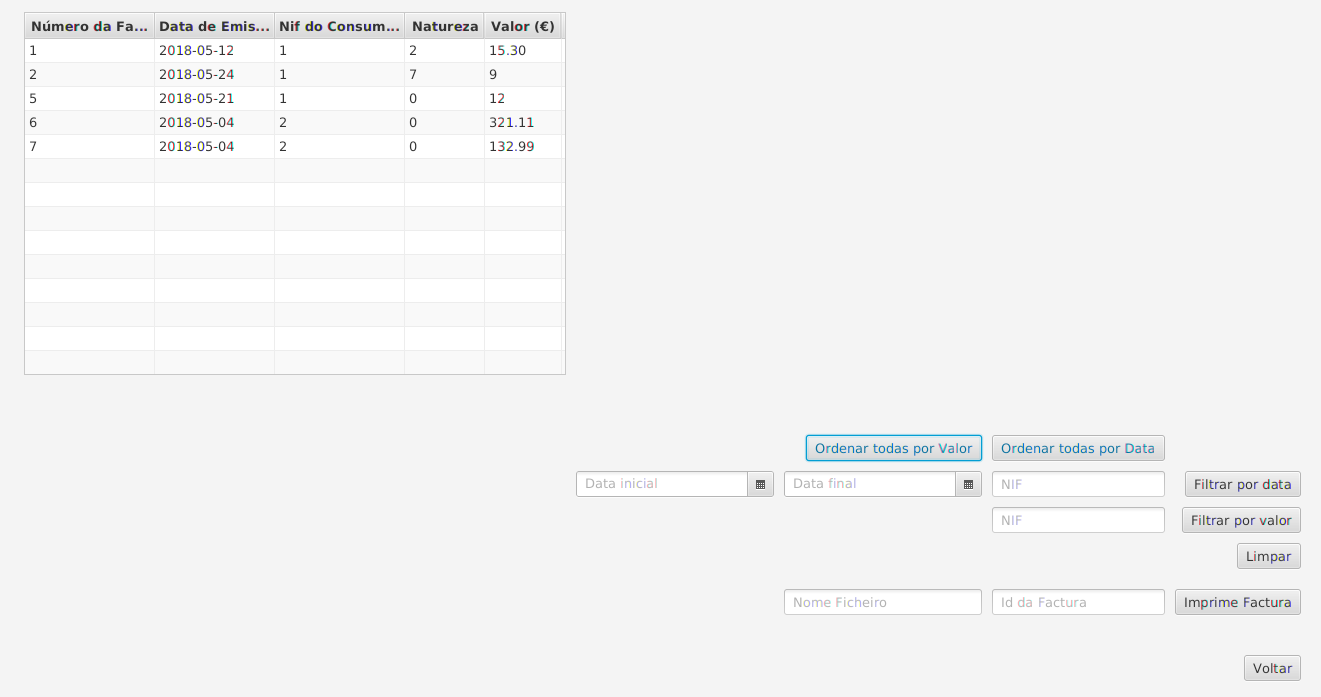
\includegraphics[scale=0.3]{imgs/consultarFaturas.png}
\caption{Aba Consultar Faturas do Contribuinte Coletivo.}
\label{img:consultarFaturas}
\end{figure}

Esse botão faz com que o método \textsf{ordenaFaturaData}, apresentado
na Figura~\ref{img:ordenaFaturaData}, seja accionado.
Este método devolve a lista das faturas da empresa com o NIF passado como
parâmetro ordenadas por data. Esta lista é então impressa na tabela,
podendo deste modo o contribuinte coletivo visualizar as suas faturas segundo esta ordem,
como podemos ver na Figura~\ref{img:consultarFaturasData}, que é o estado do programa
depois do botão ser pressionado.

\begin{figure}[H]
\centering
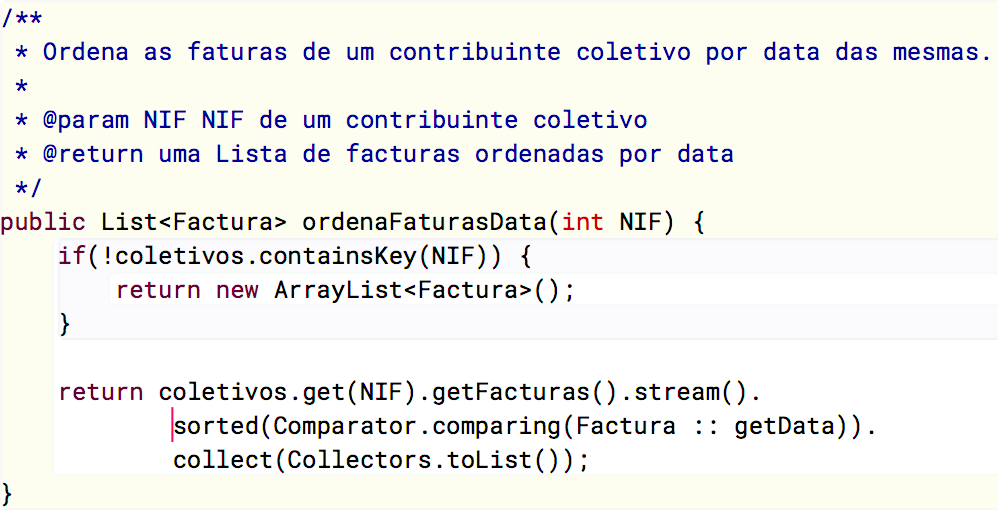
\includegraphics[scale=0.35]{imgs/ordenaFaturaData.png}
\caption{Método que ordenada as faturas de uma dada empresa por data.}
\label{img:ordenaFaturaData}
\end{figure}

\begin{figure}[H]
\centering
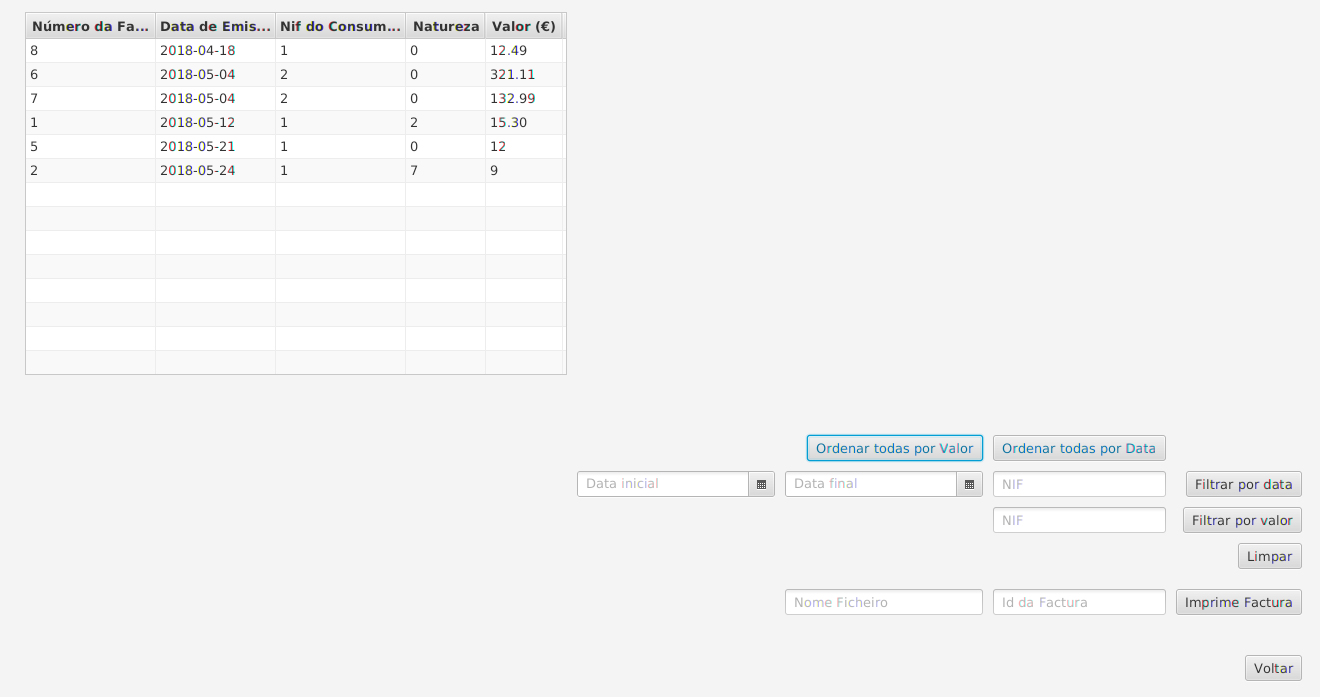
\includegraphics[scale=0.3]{imgs/consultarFaturasData.png}
\caption{Consultar Faturas por Data (Resultado Tabela).}
\label{img:consultarFaturasData}
\end{figure}

Por outro lado, poderá também carregar no botão \textbf{Ordenar todas por Valor},
que fará que com que as faturas fiquem ordenadas por valor, segundo o método
\textsf{ordenaFaturaValor}, ilustrado na Figura~\ref{img:ordenaFaturaValor}.
O resultado após pressionado o botão é o apresentado na Figura~\ref{img:consultarFaturasValor}.

\begin{figure}[H]
\centering
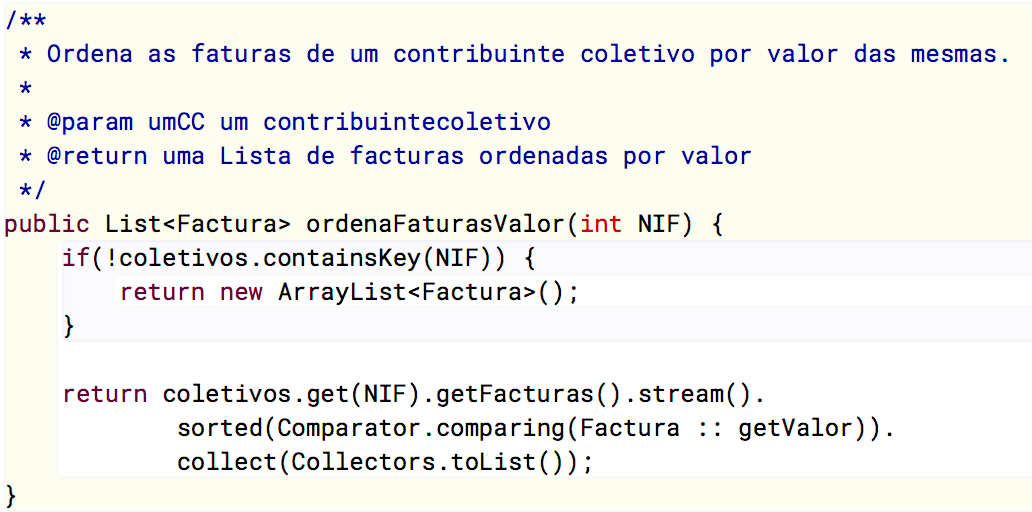
\includegraphics[scale=0.35]{imgs/ordenaFaturaValor.png}
\caption{Método que ordenada as faturas de uma dada empresa por valor.}
\label{img:ordenaFaturaValor}
\end{figure}

\begin{figure}[H]
\centering
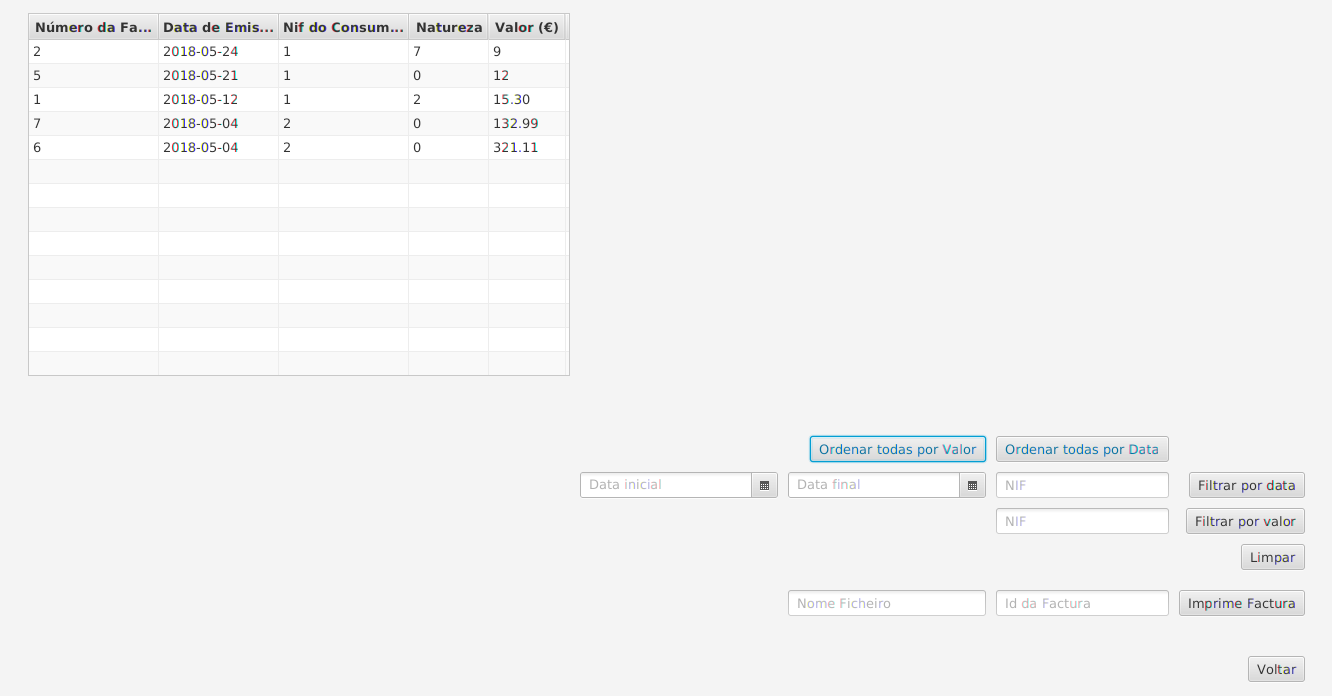
\includegraphics[scale=0.3]{imgs/consultarFaturasValor.png}
\caption{Consultar Faturas por Valor (Resultado Tabela).}
\label{img:consultarFaturasValor}
\end{figure}



\subsection{Listagem das Faturas Empresas por Contribuinte (e Data)}
\label{sec:listagemfempresascd}

\item \textbf{Obter por parte das empresas, as listagens das faturas por contribuinte num
determinado intervalo de datas.}

Para usufruir desta funcionalidade, o contribuinte coletivo apenas tem que preencher
os campos \textrm{Data Inicial}, \textrm{Data Final} e \textrm{NIF}
(do contribuinte individual) na sua dashboard
de \textbf{Consultar Facturas} (Figura~\ref{img:consultarFaturas})
e pressionar o botão \textbf{Filtrar por Data}.

É accionado o método da Figura~\ref{img:faturasPeriodoContribuinte},
e o procedimento é exatamente igual ao mencionado na secção anterior
(Secção~\ref{sec:listagemfempresas}), irá aparecer na tabela as faturas do
determinado contribuinte individual realizadas no intervalo de tempo
escolhido.

\begin{figure}[H]
\centering
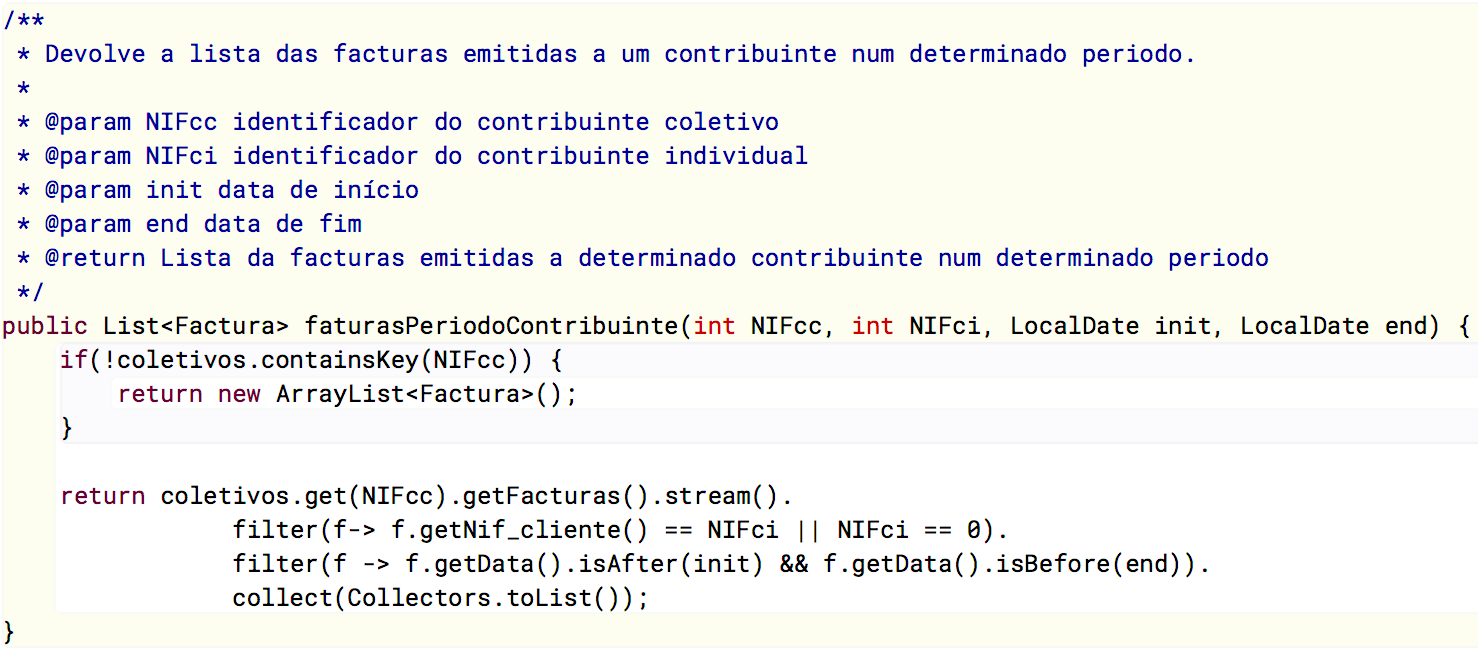
\includegraphics[scale=0.35]{imgs/faturasPeriodoContribuinte.png}
\caption{Método que retorna as faturas de uma dada empresa passadas para um determinado contribuinte,
no intervalo de tempo mencionados.}
\label{img:faturasPeriodoContribuinte}
\end{figure}



\subsection{Listagem das Faturas Empresas por Contribuinte (e Valor)}
\label{sec:listagemfempresascv}

\item \textbf{Obter por parte das empresas, as listagens das faturas por contribuinte ordenadas
por valor decrescente de despesa.}

Para esta funcionalidade o raciocínio é igual ao anterior mencionado.
O contribuinte coletivo preenche o campo NIF do contribuinte individual
(na segunda linha que pede o NIF), na dashboard
\textbf{Consultar Facturas} (Figura~\ref{img:consultarFaturas}),
e pressionar \textbf{Filtrar por Valor}.

As faturas do contribuinte individual escolhido aparecerão na tabela,
ordenadas por valor decrescente de despesa (o método que é chamado
é o método apresentado na Figura~\ref{img:faturasValorContribuinte}).

\begin{figure}[H]
\centering
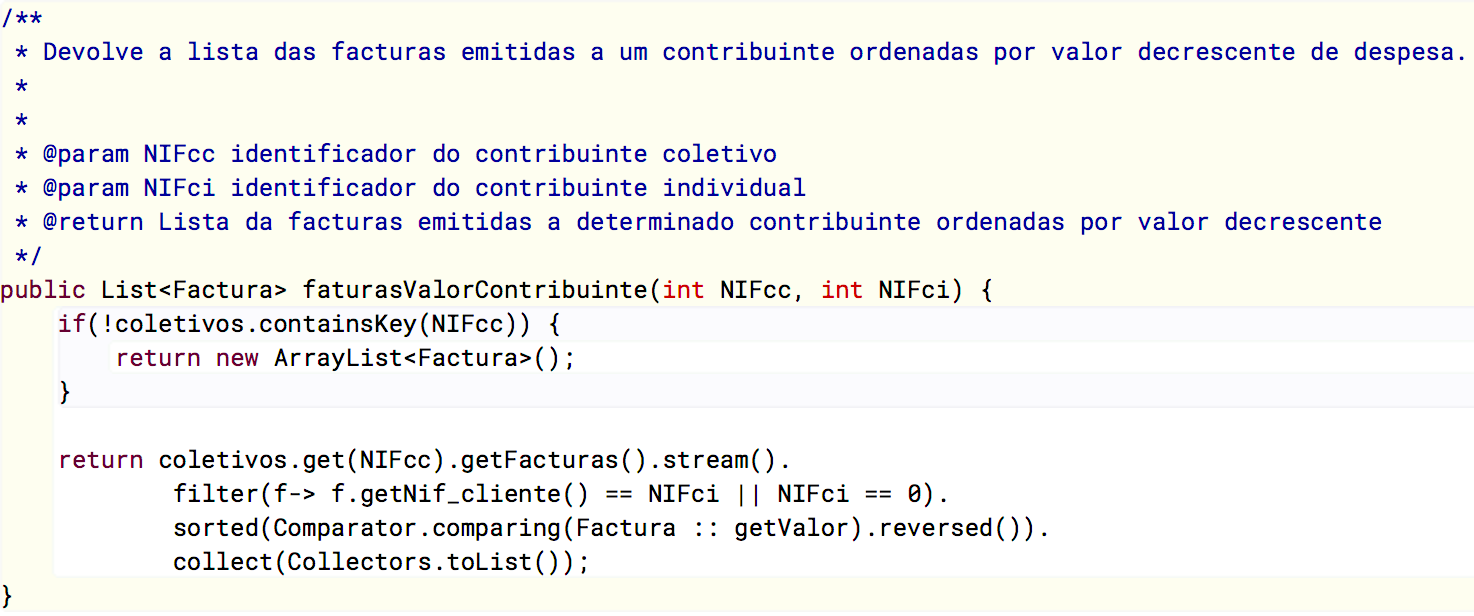
\includegraphics[scale=0.35]{imgs/faturasValorContribuinte.png}
\caption{Método que retorna as faturas de uma dada empresa passadas para um determinado contribuinte,
ordenadas por valor decrescente de despesa.}
\label{img:faturasValorContribuinte}
\end{figure}



\subsection{Total faturado por uma empresa num determinado período}
\label{sec:totalfaturaempperio}

\item \textbf{Indicar o total faturado por uma empresa num determinado período.}

O contribuinte coletivo tem ainda a oportunidade de consultar o valor total faturado
num determinado período. Para isso, basta clicar, através da sua dashboard
(Figura~\ref{img:dashboardcoletivo}), no botão \textbf{Consultar Valores de Facturas}. Abrirá
o seguinte separador:

\begin{figure}[H]
\centering
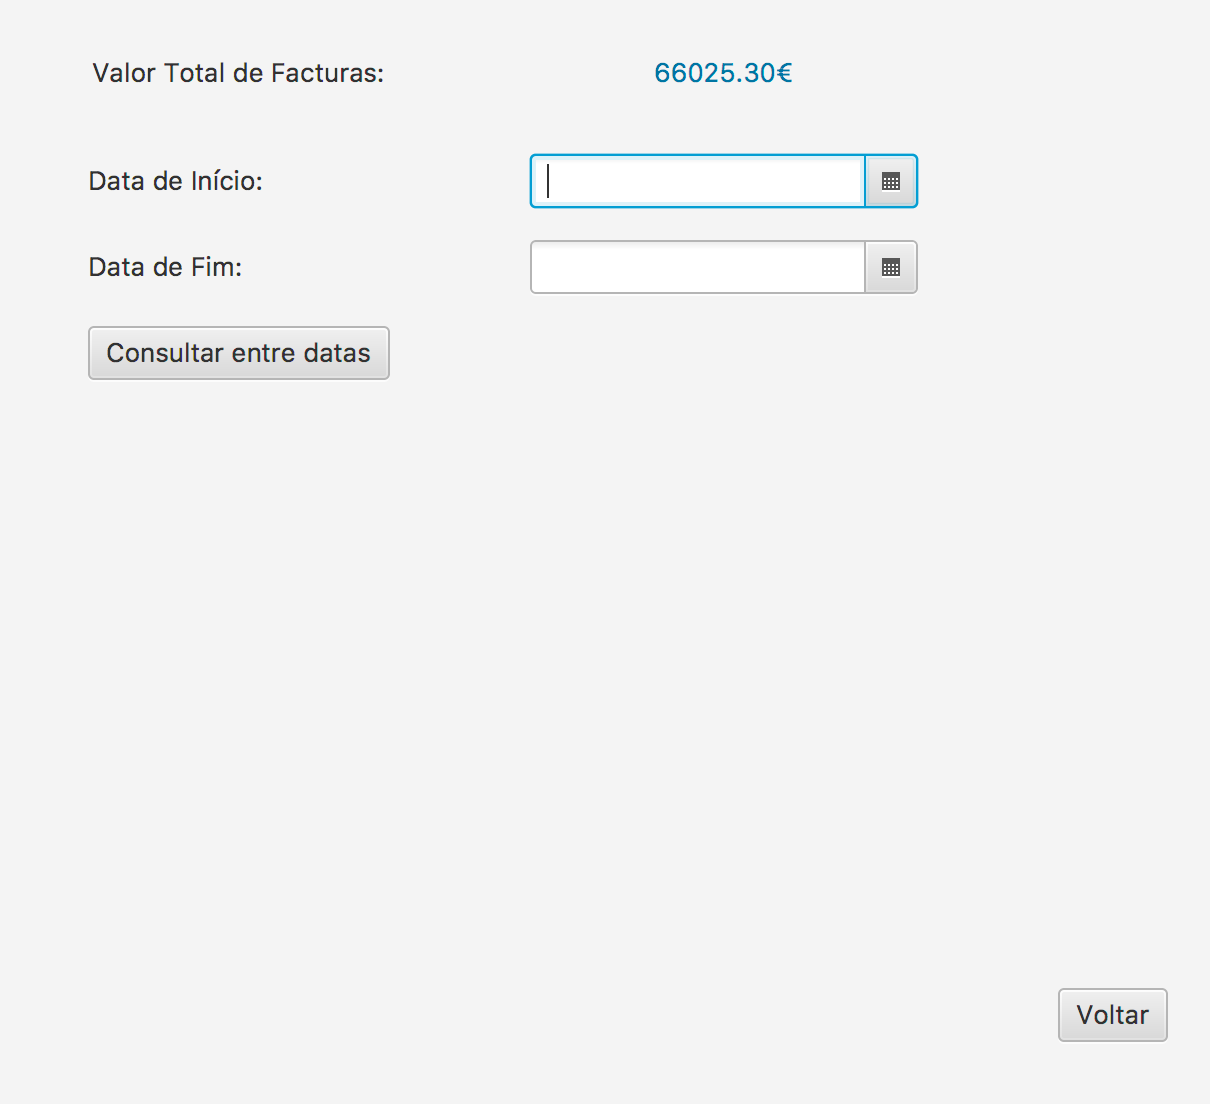
\includegraphics[scale=0.35]{imgs/totalFacturadoScreen.png}
\caption{Consultar Valores de Facturas Ecrã.}
\label{img:totalFacturadoScreen}
\end{figure}

E, aqui, o contribuinte coletivo pode selecionar a Data de Início e a Data
de Fim e \textbf{Consultar entre datas} o valor faturado. Depois de escolhidas
as datas e selecionado o botão, irá aparecer
numa Label o valor correspondente
(tal como apresentado na Figura~\ref{img:totalFacturaIntervaloScreen}).

\begin{figure}[H]
\centering
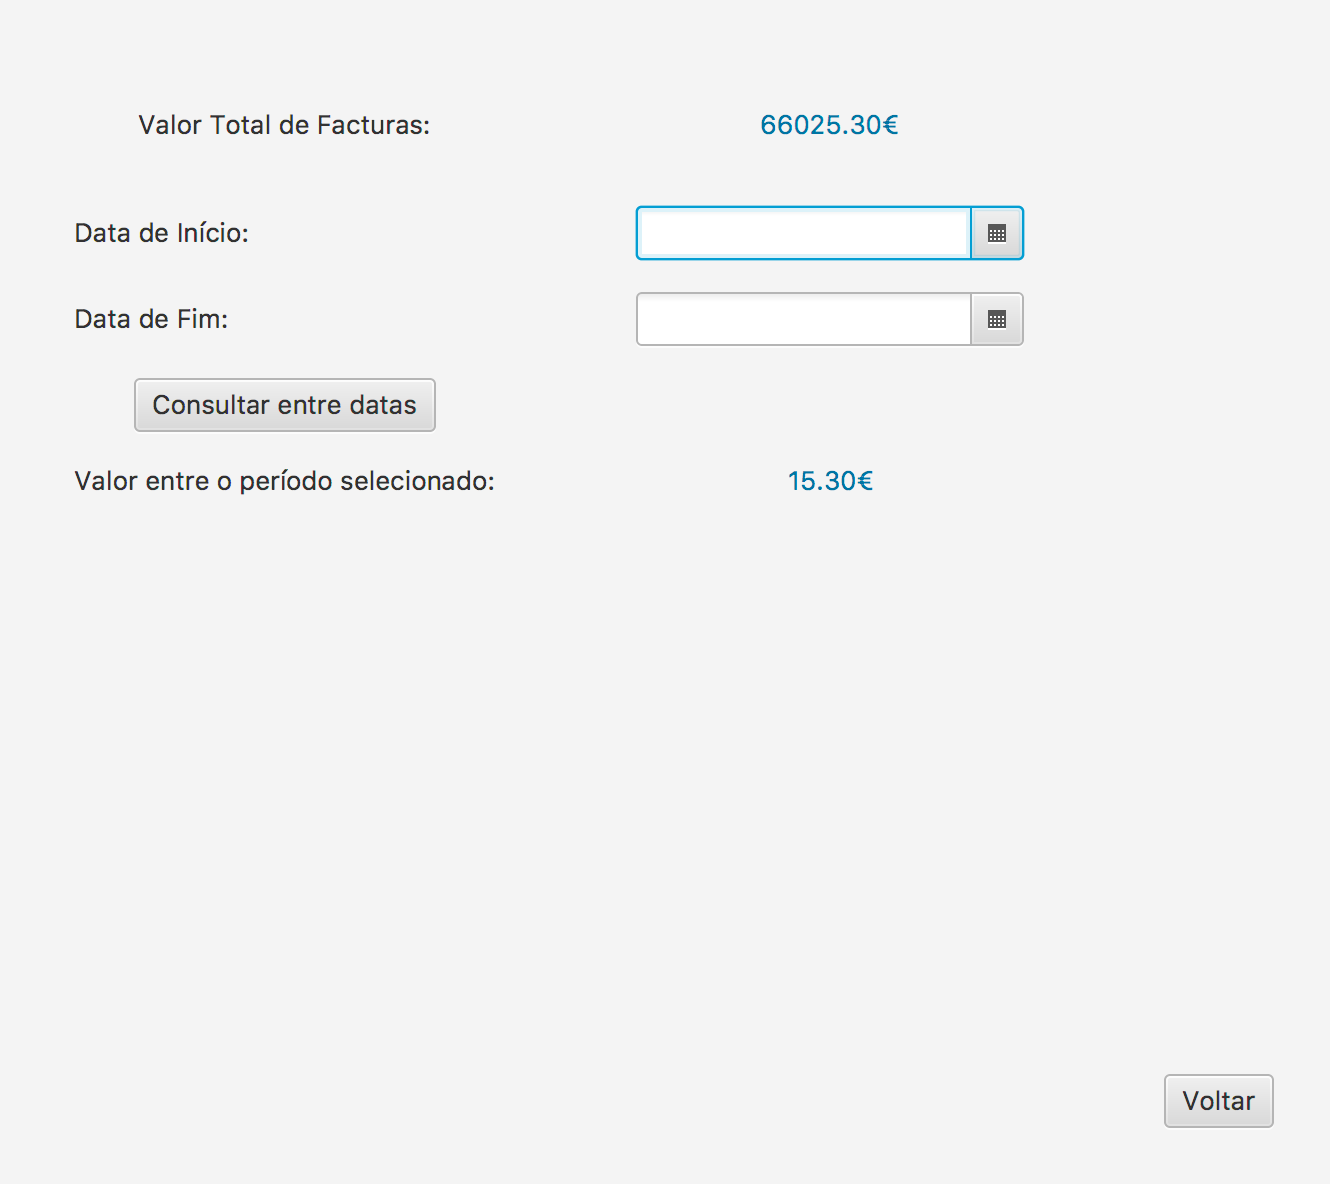
\includegraphics[scale=0.35]{imgs/totalFacturaIntervaloScreen.png}
\caption{Consultar Valores de Facturas Exemplo de Intervalo Ecrã.}
\label{img:totalFacturaIntervaloScreen}
\end{figure}


Os métodos chamados para tal são os métodos apresentados na Figura~\ref{img:totalFacturado}
e Figura~\ref{img:totalFacturadoCC}, respetivamente.

\begin{figure}[H]
\centering
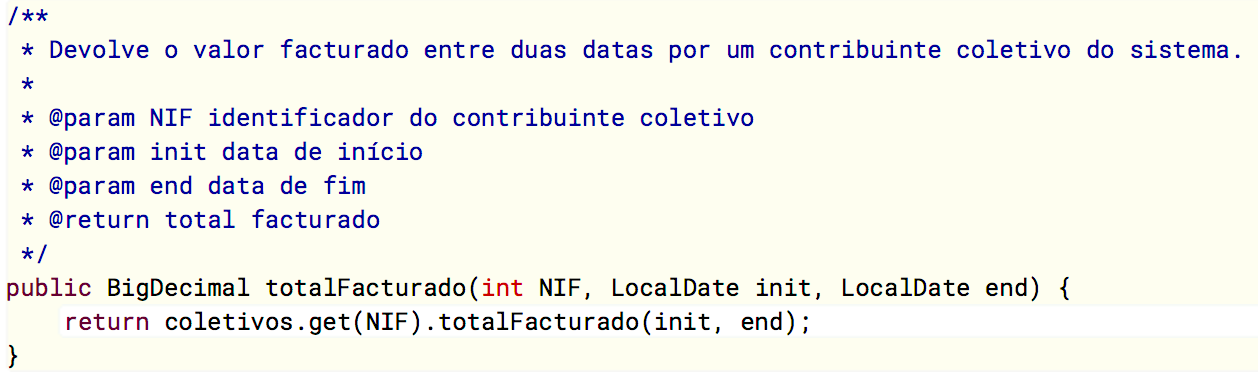
\includegraphics[scale=0.35]{imgs/totalFacturado.png}
\caption{Método da classe JavaFactura que calcula o total fatura
por uma empresa num determinado período.}
\label{img:totalFacturado}
\end{figure}

\begin{figure}[H]
\centering
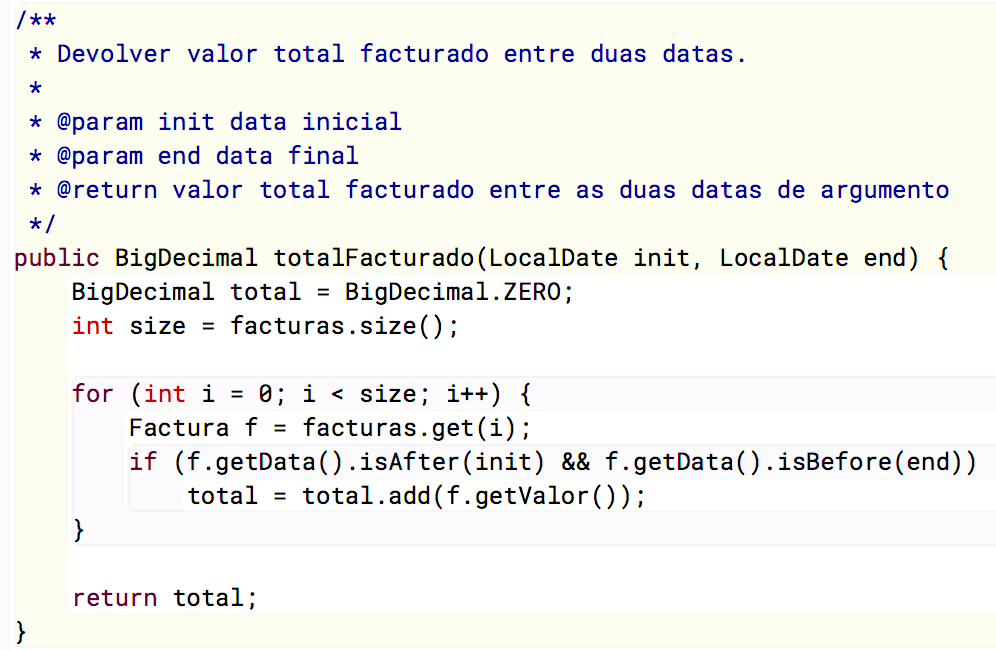
\includegraphics[scale=0.35]{imgs/totalFacturadoCC.png}
\caption{Método da classe ContribuinteColetivo que efetivamente calcula o valor pedido.}
\label{img:totalFacturadoCC}
\end{figure}



\subsection{Coleção dos 10 Contribuintes que mais gastam}
\label{sec:colecao10contr}

\item \textbf{Determinar a relação dos 10 contribuintes que mais gastam em todo
o sistema (esta operação
deve ser só disponibilizada para o administrador da aplicação).}

O administrador do sistema pode consultar a coleção dos 10 contribuintes
que mais gastam. Para tal, carregam no botão \textbf{10 contribuintes que mais gastam},
presente na sua dashboard de administrador (Figura~\ref{img:dashboardadmin}).

Será apresentado o separador na imagem seguinte, onde estão impressos os NIFs
dos 10 contribuintes que mais gastaram e respetivo valor de gasto.

\begin{figure}[H]
\centering
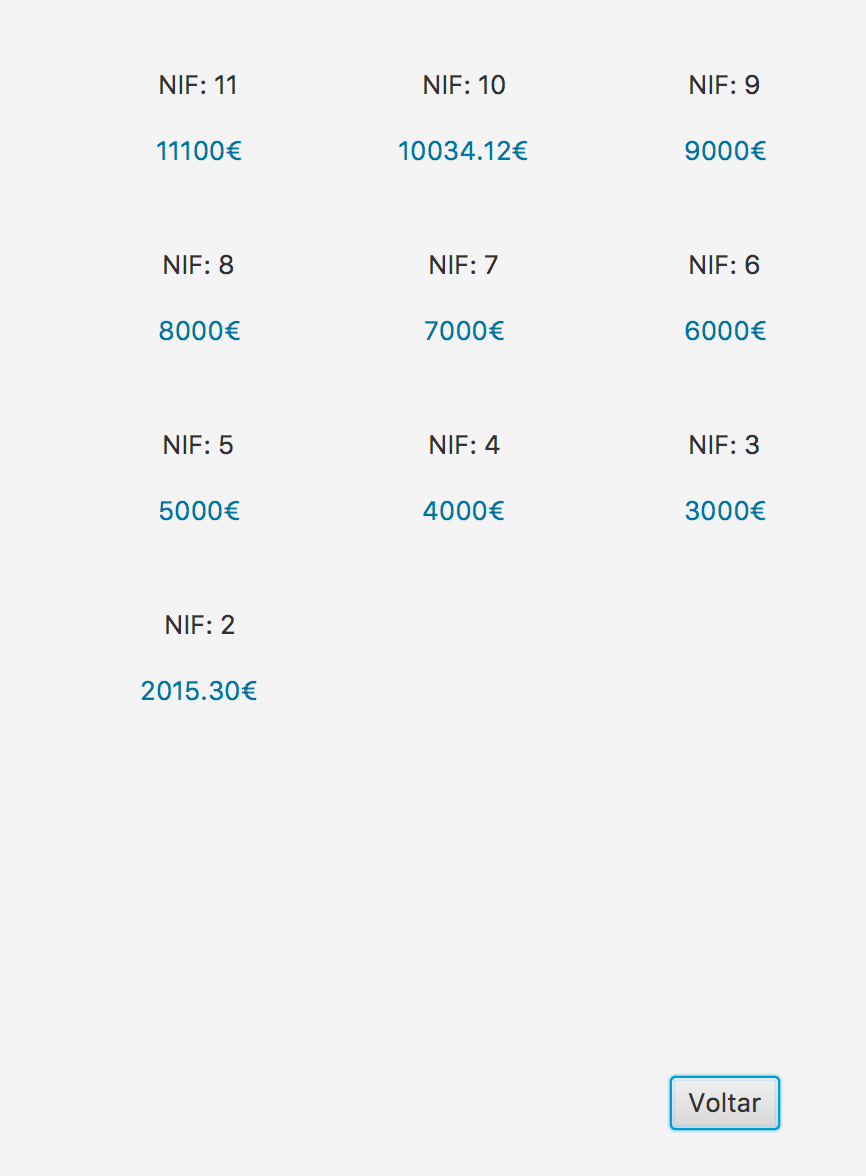
\includegraphics[scale=0.35]{imgs/10contribuintesScreen.png}
\caption{Aba 10 contribuintes que mais gastam.}
\label{img:10contribuintesScreen}
\end{figure}

Os métodos que são utilizados para tal são os métodos presentes na seguinte
figura:

\begin{figure}[H]
\centering
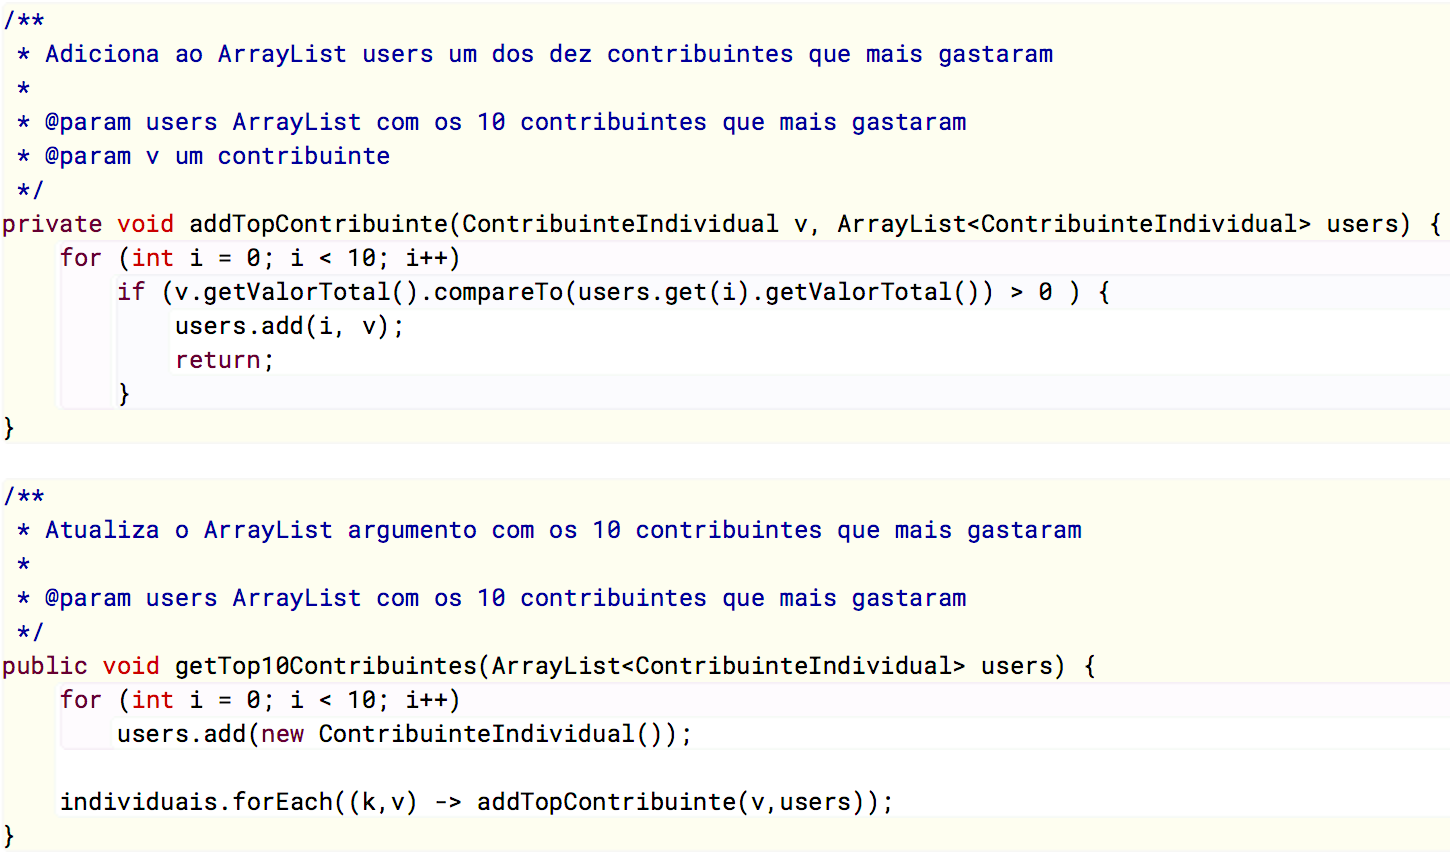
\includegraphics[scale=0.35]{imgs/10contribuintesMetodos.png}
\caption{10 contribuintes que mais gastam (Métodos).}
\label{img:10contribuintesMetodos}
\end{figure}



\subsection{Coleção X Empresas}
\label{sec:colecaoxempresas}

\item \textbf{Determinar a relação das X empresas que têm mais faturas em todo o sistema e
o montante de deduções fiscais que as despesas registadas (dessas empresas)
representam (esta operação deve ser só disponibilizada para o administrador da aplicação).}

Para determinar a coleção das X empresas que têm mais faturas e respetivo
o montante de deduções fiscais foi utilizado o método da
Figura~\ref{img:colecaoXempresasMetodos}.

\begin{figure}[H]
\centering
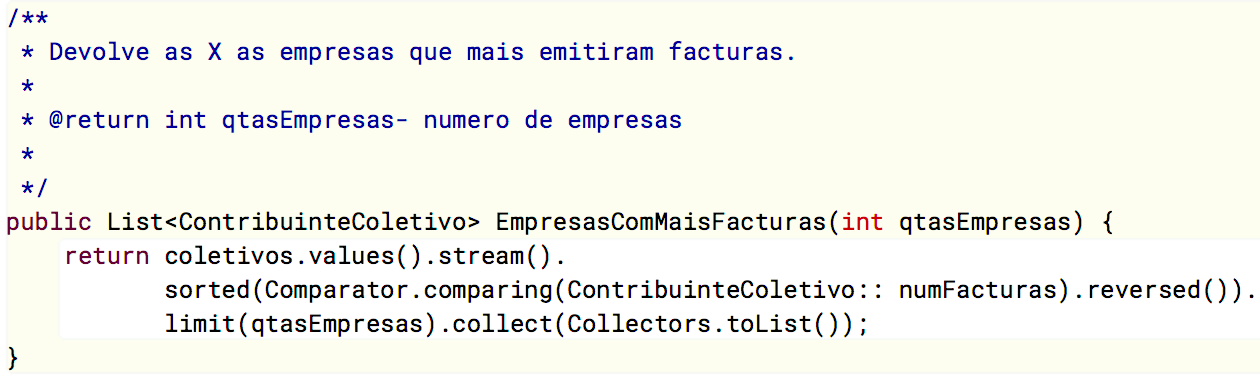
\includegraphics[scale=0.35]{imgs/colecaoXempresasMetodos.png}
\caption{Coleção X Empresas Métodos.}
\label{img:colecaoXempresasMetodos}
\end{figure}

Para consultar esta funcionalidade o administrador da aplicação deverá selecionar
o botão \textbf{Empresas com mais facturas emitidas},
presente na sua dashboard (Figura~\ref{img:dashboardadmin}).

Aparecerá o seguinte separador:


\begin{figure}[H]
\centering
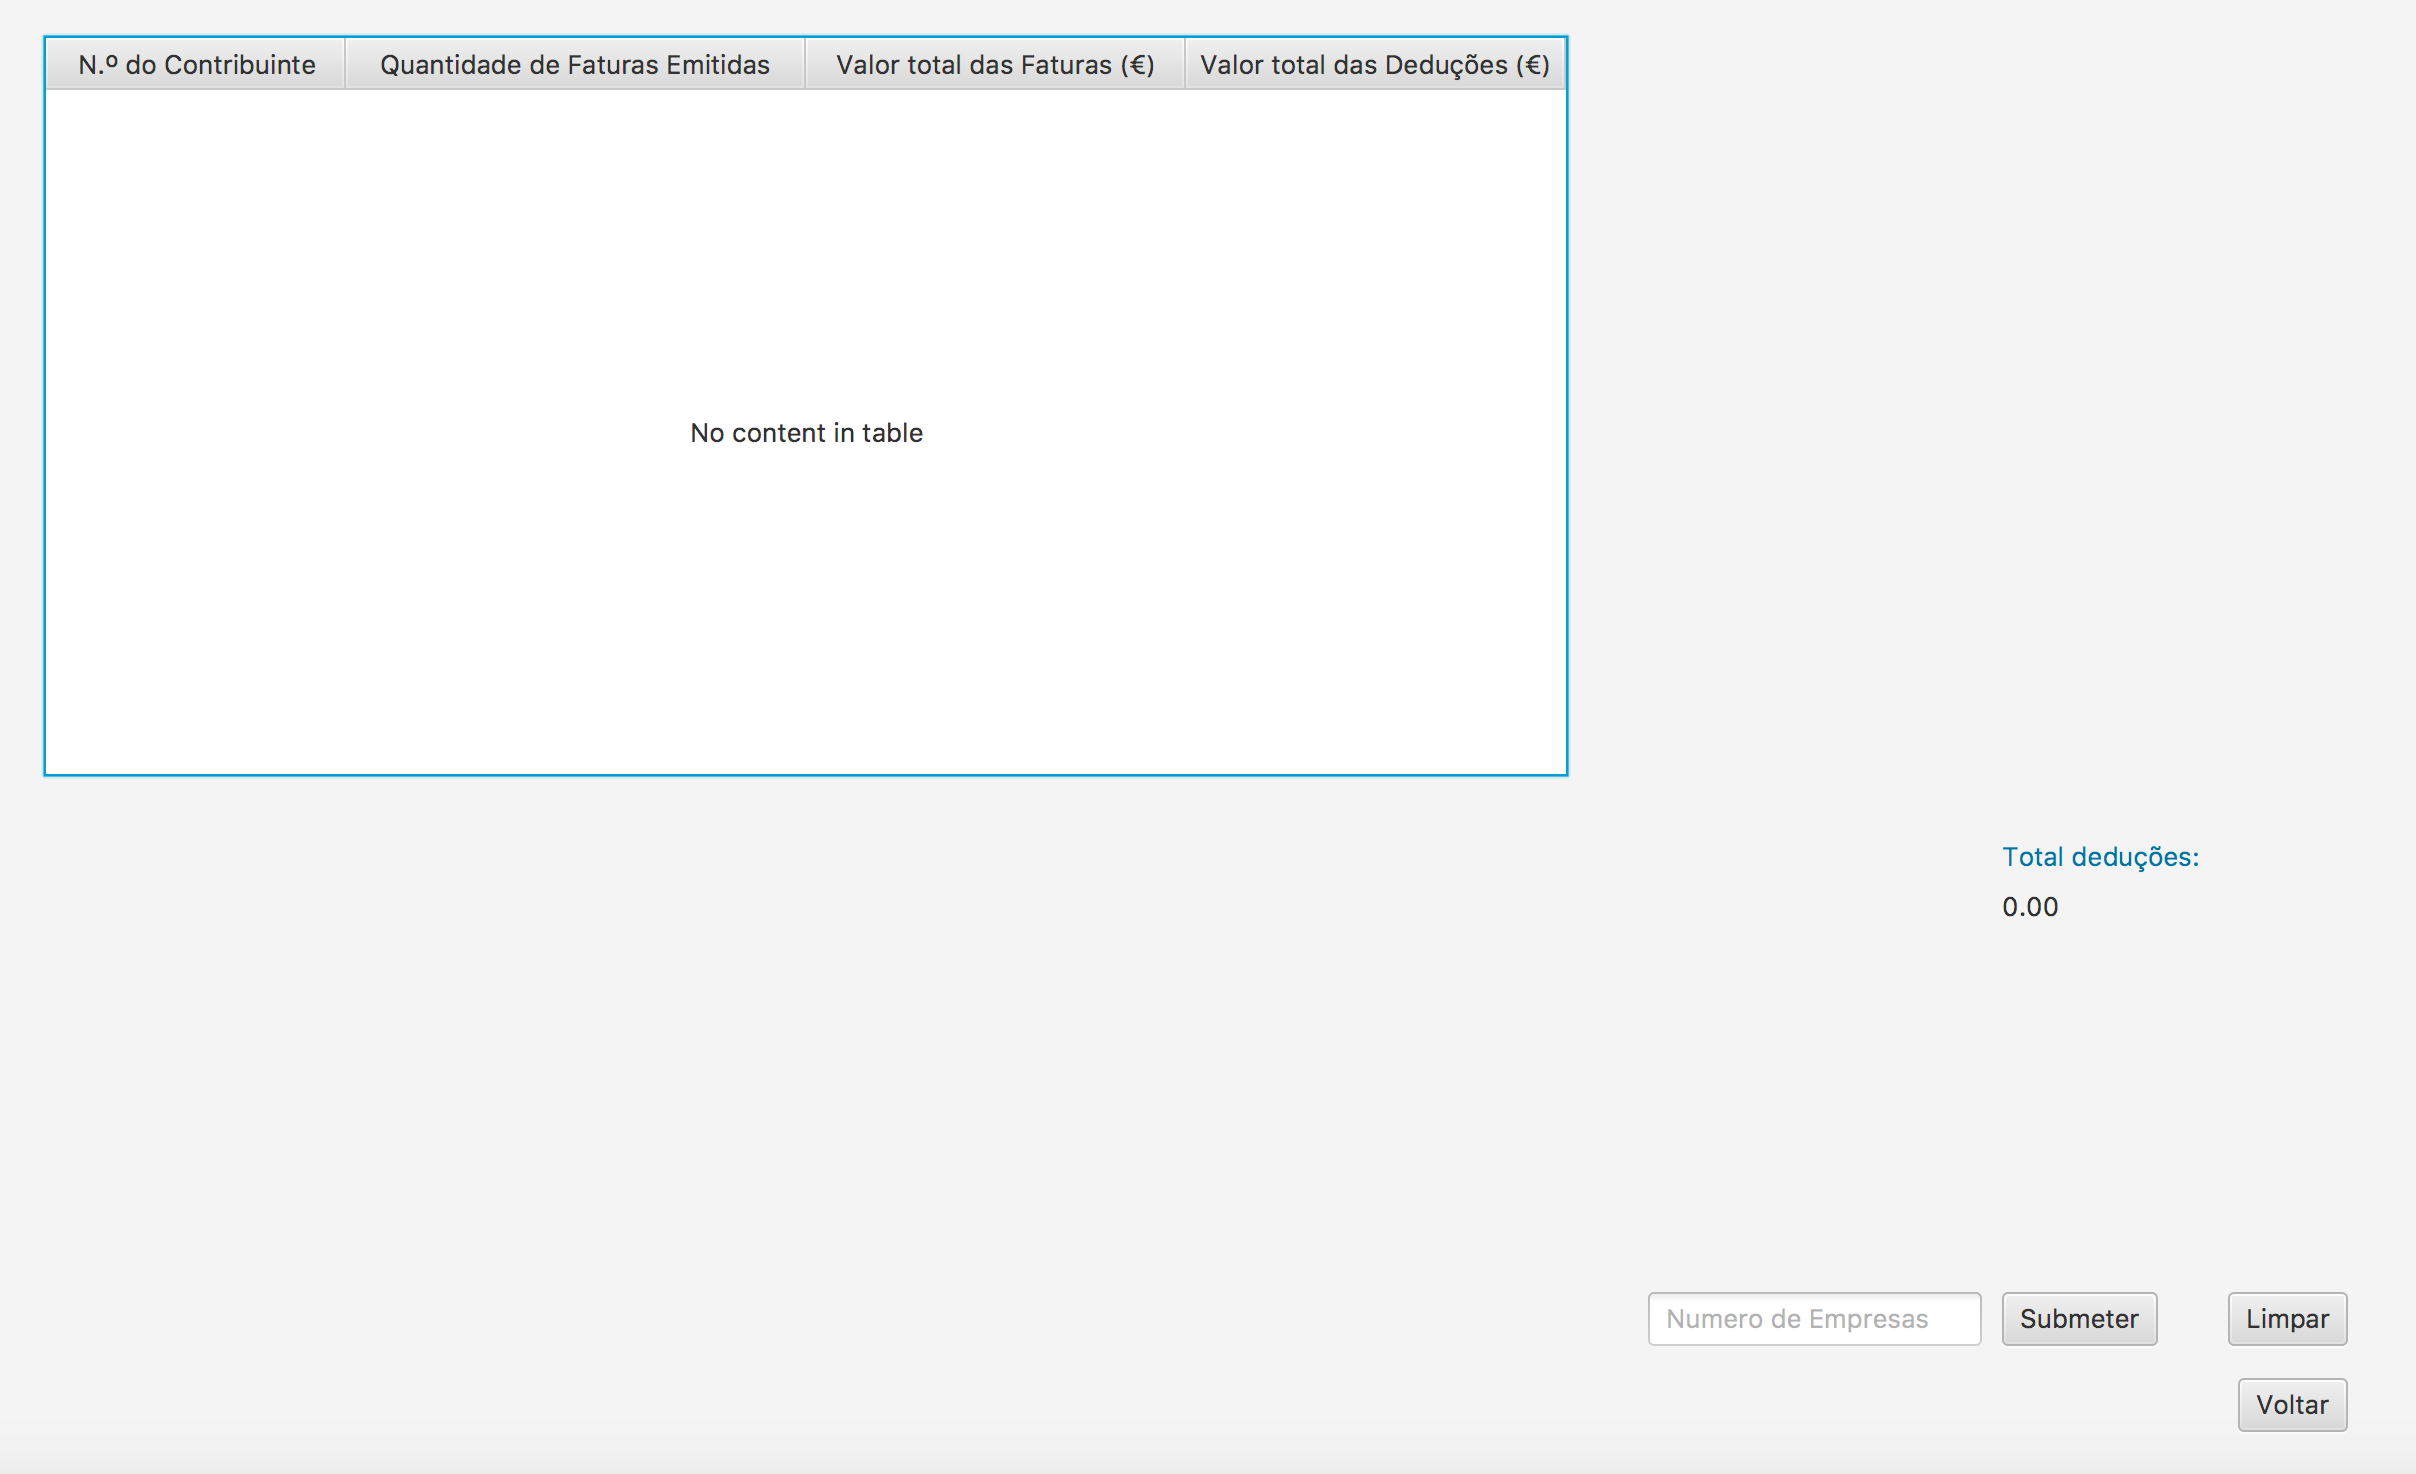
\includegraphics[scale=0.35]{imgs/colecaoXempresasScreen.png}
\caption{Coleção X Empresas Ecrã.}
\label{img:colecaoXempresasScreen}
\end{figure}

Preenchendo o campo \textsf{Numero de Empresas}, e carregando em
\textbf{Submeter}, aparecerá na tabela as informações pretendidas.

Para facilitar o preenchimento da tabela foi criada uma classe auxiliar chamada
\textsf{EmpresasTop} dentro da classe \textsf{GUI}.



\subsection{Gravar Estado da Aplicação em Ficheiro}
\label{sec:gravarestado}

\item \textbf{Gravar o estado da aplicação em ficheiro,
para que seja possível retomar mais tarde a execução.}

Para gravarmos e retomarmos o estado da nossa aplicação usamos a
API java.io e implementamos os métodos \textsf{guardaEstado} e \textsf{carregaEstado},
sendo que o primeiro guarda o estado da aplicação em binário e o segundo recupera esse
mesmo estado. Estes métodos utilizam as classes FileOutputStream e FileInputStream
os quais permitem criar uma stream de escrita e de leitura, respetivamente.

Para tanto, todas as classes cujas instâncias devem escrever e ler os seus atributos
em formato binário para e de um ficheiro implementam a interface Serializable. Este
processo, conhecido como serialização, é inicializado pela escrita do JavaFactura através
do método \textsf{writeObject} da classe ObjectOutputStream e todas as referências a outros objetos
a partir do JavaFactura são recursivamente escritas.

Para realizar a ``desserialização" dos bytes escritos para o ficheiro, ou a leitura desses bytes
utilizamos o método \textsf{readObject} da clase ObjectInputStream. \par

Em simultâneo, usando FileOutputStream e FileInputStream, é também guardado em
ficheiro, em modo de texto, o valor da variável de classe de Factura, nextID,
que representa o Id único da próxima factura a ser emitida.
\vspace{1.5cm}



\subsection{Familias Numerosas e Empresas do Interior}
\label{sec:familiaNumerosa_EmpresasInterior}


\item\textbf{Gestão da definição do número de filhos para qualificação de uma
família como sendo numerosa}
\vspace{0.5cm}

Uma família numerosa é aquela que tem mais do que 4 dependentes. Para que o nosso
programa considere uma família numerosa o agregado familiar terá de ser constituído
por, pelo menos, um contribuinte que assuma a sua direção e cindo ou mais dependentes.
O programa faz essa gestão através do método \emph{addNovoDependenteAgregado}.

\vspace{0.5cm}
\begin{figure}[H]
\centering
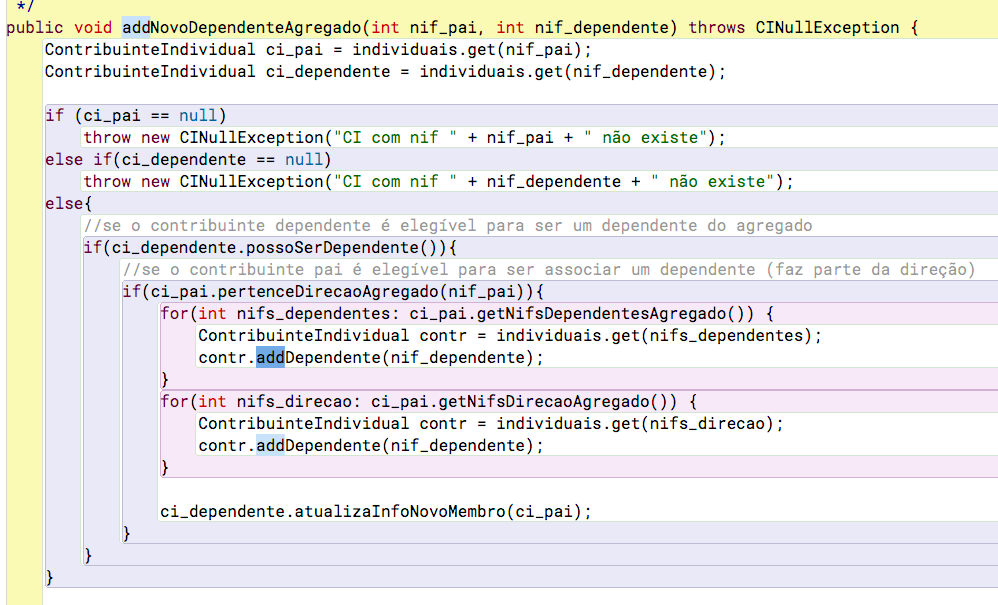
\includegraphics[scale=0.35]{imgs/addDependente1.png}
\label{img:addDependente1}
\end{figure}

\begin{figure}[H]
\centering
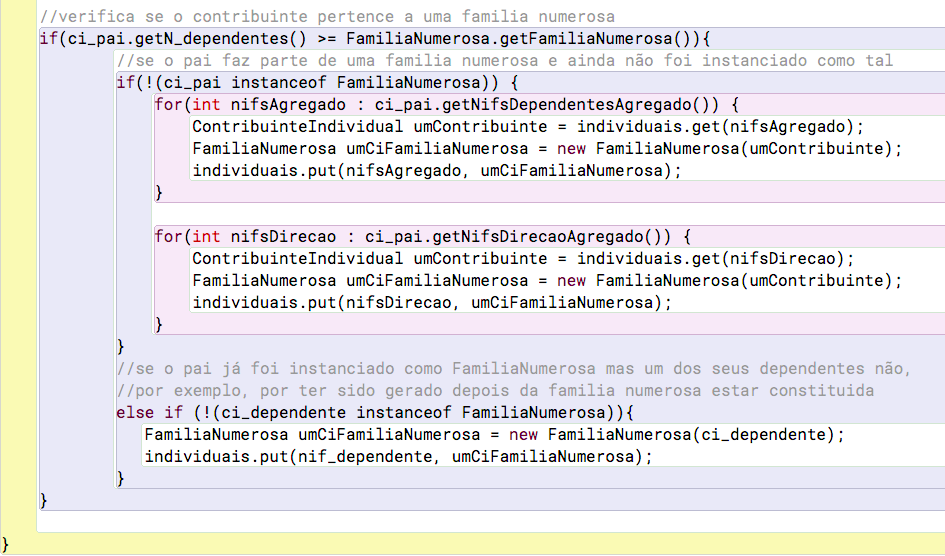
\includegraphics[scale=0.35]{imgs/addDependente2.png}
\caption{Método \emph{addNovoDependenteAgregado}.}
\label{img:addDependente2}
\end{figure}


Sempre que um dependente é adicionado a um agregado, verifica-se o número total
de dependentes que o integram e no caso de atingir os 5, todos os contribuintes individuais
que compõem esse agregado passam a ser instâncias de \emph{FamiliaNumerosa}.


A constituição do agregado é explicada detalhadamente na Secção~\ref{sec:criacaodeagregados}.



\vspace{0.5cm}

\item\textbf{Tratamento priveligiado da Empresa do Interior.}
\end{itemize}
\vspace{0.5cm}

Conforme referimos anteriormente, em determinadas situações o cálculo das deduções
tem em consideração a localização da sede da empresa. Por isso, aquando do registo
do contribuinte coletivo, Figura~\ref{img:criarcc}, é necessário introduzir o distrito da
sede da empresa, visto que se a empresa estiver sediada num concelho do interior do
país e se efetuar uma transação no setor automóvel, restauração, motociclos ou transportes
o adquirente do serviço ou do bem beneficiará de uma dedução fiscal superior.
Essa funcionalidade é implementada pelo código infra, o qual cria os 18 concelhos,
associa-lhes o valor percentual que irá acrescer à percentagem de dedução estipulada
nos setores de atividade acima mencionados e insere-os na variável de classe atividades.


\vspace{1.5cm}



\subsection{Criação de Agregados}
\label{sec:criacaodeagregados}

No nosso programa implementamos também uma forma simples e realista de criar agregados
familiares.

Assim, existem 2 entidades dentro de um agregado: os diretores do agregado e os
dependentes do agregado (como já foi mencionado na Secção~\ref{sec:contribuinteindividual}).

Como tal, toda a gente deve inserir-se (caso de diretor) ou ser inserida
(caso de dependente) em um desses setores.

Para se inserir como diretor do agregado o contribuinte tem que, dentro da sua dashboard
(Figura~\ref{img:dashboardindividual}), aceder ao separador \textbf{Direção do
Agregado}. Dentro deste separador, demonstrado na Figura~\ref{img:direcaodoagregado},
o utilizador tem a hipótese de \textbf{Fazer parte da direção deste agregado}. Se o fizer,
o mesmo passa imediatamente a ser o diretor do seu agregado.

\begin{figure}[H]
\centering
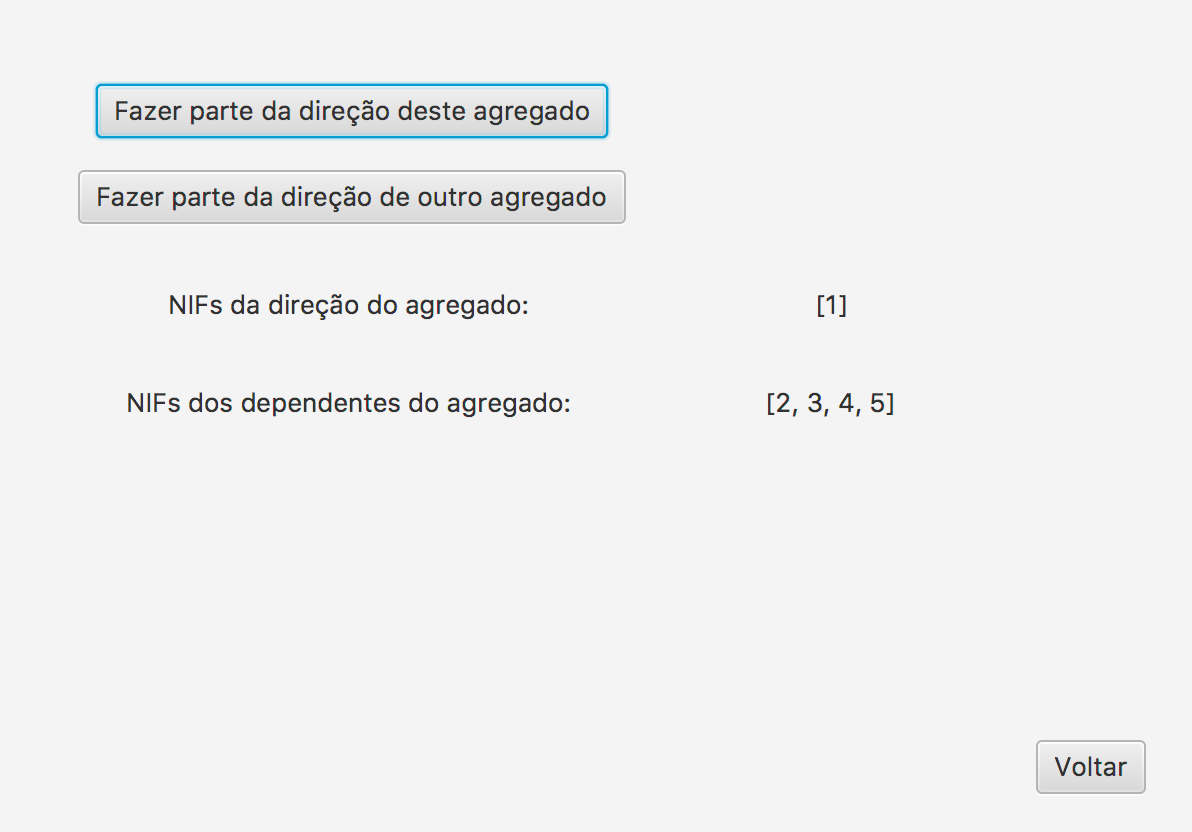
\includegraphics[scale=0.35]{imgs/direcaodoagregado.png}
\caption{Ecrã do Agregado.}
\label{img:direcaodoagregado}
\end{figure}

Um diretor de um agregado pode adicionar dependentes acedendo, a partir da sua dashboard
(Figura~\ref{img:dashboardindividual}), ao separador \textbf{Associar Dependentes}.
Dentro desta aba (apresentada na Figura em seguida) o contribuinte tem que digitar o NIF
do dependente e carregar em Registar.

\begin{figure}[H]
\centering
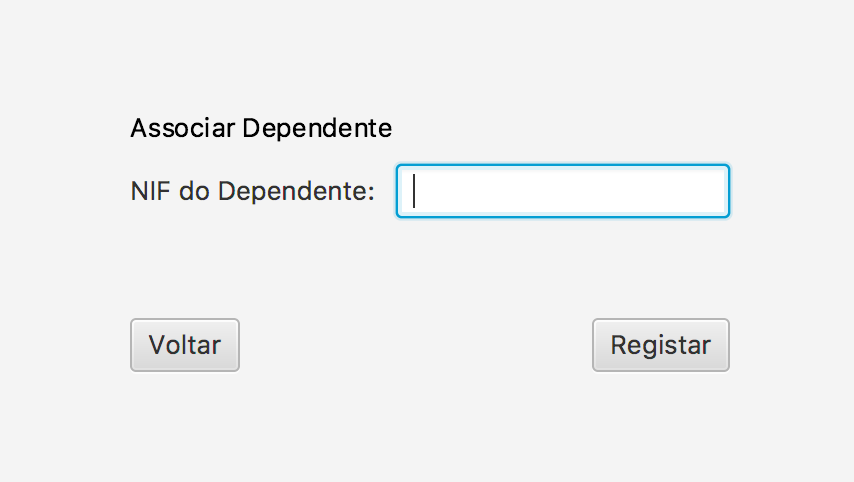
\includegraphics[scale=0.35]{imgs/associardependente.png}
\caption{Ecrã Associar Dependente.}
\label{img:associardependente}
\end{figure}

No entanto algumas regras têm que
ser cumpridas em ambos os casos, passo a enumerar:


\begin{itemize}
\item \textbf{Ser diretor de um agregado:}

\begin{enumerate}
\item Não pode ser dependente de nenhum agregado;
\item Direção do agregado ainda não pode estar cheia
(número de diretores é no máximo 2).
\end{enumerate}


\item \textbf{Ser dependente de um agregado:}

\begin{enumerate}
\item Não fazer parte de nenhum agregado, quer como dependente, quer como diretor;
\item O contribuinte que o está a tentar adicionar tem que ser diretor de um agregado.
\end{enumerate}
\end{itemize}

Assim, quando algum contribuinte individual é adicionado por um diretor a um agregado
as informações do agregado (valores das deduções, despesas, NIFs dos outros membros do
agregado e respetivo número (de dependentes e de diretores)) são atualizadas em ambos
os contribuintes.

\vspace{1cm}

Os contribuintes individuais têm ainda a oportunidade de se associarem a outro agregado,
isto é, por exemplo, se existem dois agregados sendo um deles constituído por um pai e dois
filhos e o outro constituído por uma mãe e um filho tanto o pai como a mãe dos diferentes
agregados podem optar por
se juntarem e com isto juntarem também os seus dependentes, passando a serem um só agregado
com dois pais e três filhos. As informações do novo agregado são respetivamente atualizadas
em todos os membros.

Esta opção está disponível quando o utilizador acede ao botão
\textbf{Fazer parte da direção de outro agregado}, presente na aba
\textbf{Direção do Agregado} (Figura~\ref{img:direcaodoagregado}).
Esta será a dashboard apresentada:

\begin{figure}[H]
\centering
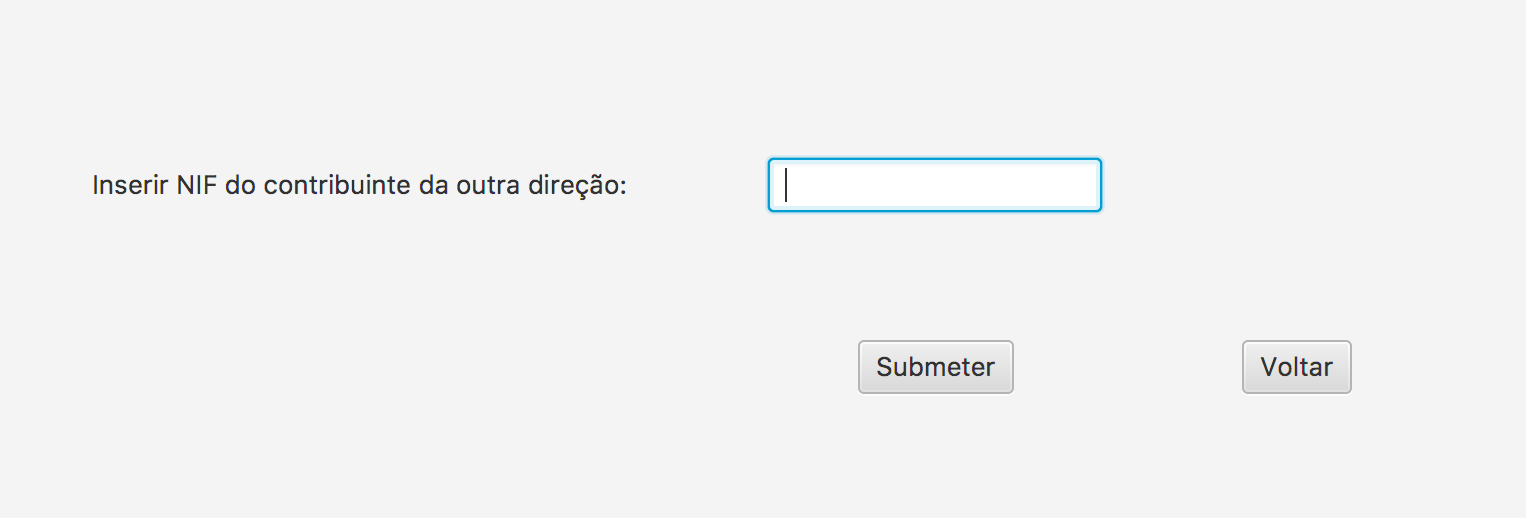
\includegraphics[scale=0.35]{imgs/direcaooutroagregado.png}
\caption{Ecrã intenção de se associar a outro agregado.}
\label{img:direcaooutroagregado}
\end{figure}

É de salientar que terá que ser um dos dois diretores do agregado a adicionar o outro
diretor, e que ambos os agregados só podem ter um membro diretor para deste modo
o agregado se juntar e ficarem os dois como diretores (como já foi mencionado o
número máximo de diretores é 2) .

\vspace{0.2cm}

Esta implementação facilitou o cálculo das deduções e despesas e a
implementação do conceito de Familia Numerosa.



\subsection{Download e Impressão de Facturas}
\label{sec:imprimirfacturas}

Tanto um contribuinte individual como um contribuinte coletivo tem disponível
uma ferramenta, a partir do ecrã de consulta de faturas disponível a cada um,
para fazer download de um fatura, em formato HTML, que poderá
depois ser impressa através de uma navegador de Internet.

\begin{figure}[H]
\centering
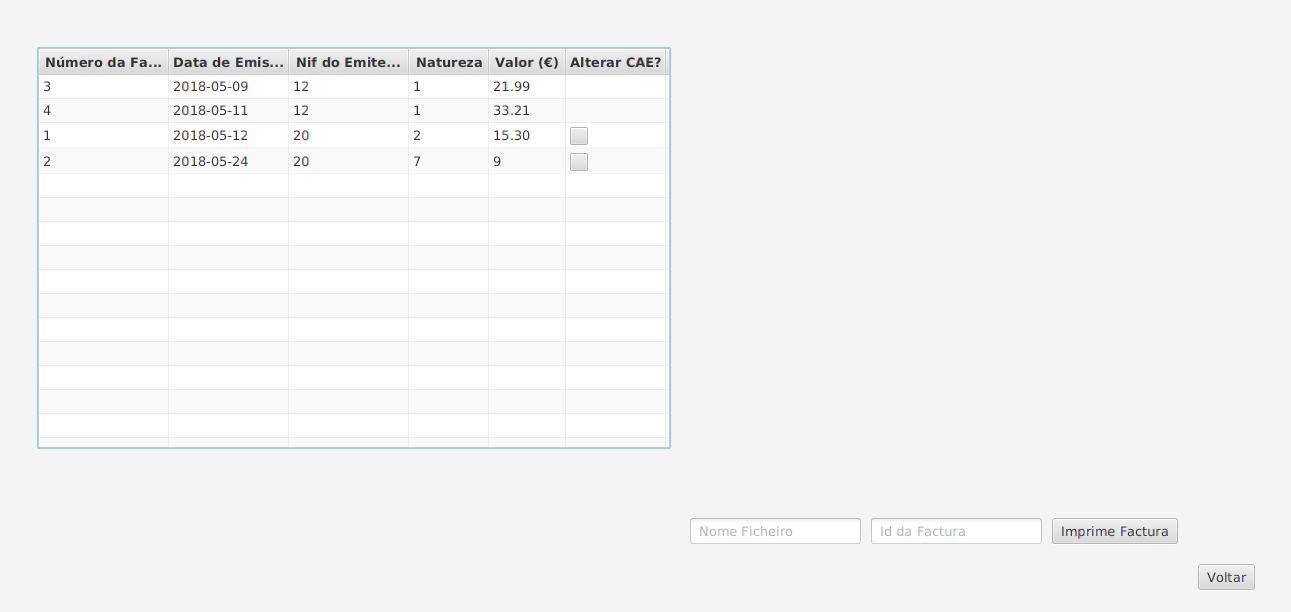
\includegraphics[scale=0.35]{imgs/consultafaturas.png}
\caption{Download de Factura por parte do Contribuinte Individual.}
\label{img:downloadfaturaci}
\end{figure}

\begin{figure}[H]
\centering
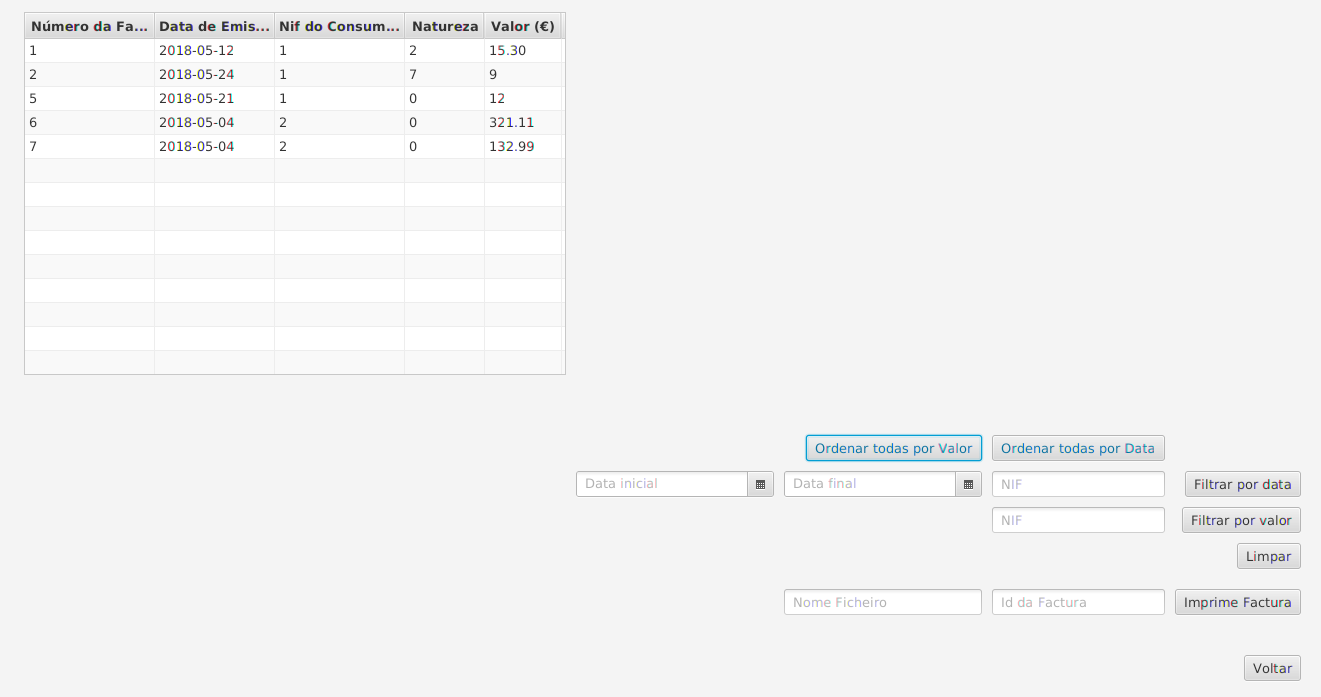
\includegraphics[scale=0.35]{imgs/consultarFaturas.png}
\caption{Download de Factura por parte do Contribuinte Coletivo.}
\label{img:downloadfaturacc}
\end{figure}

Esta é uma funcionalidade relativamente simples, existe na aplicação um
layout de HTML/CSS na qual são introduzidos os dados da factura e das
entidades intervenientes e, de seguida, o resultado é, através do recurso à API
FileOutputStream, impresso para um ficheiro cujo nome pode ou não ser definido
pelo utilizador, em codificação UTF-8.

\begin{figure}[H]
\centering
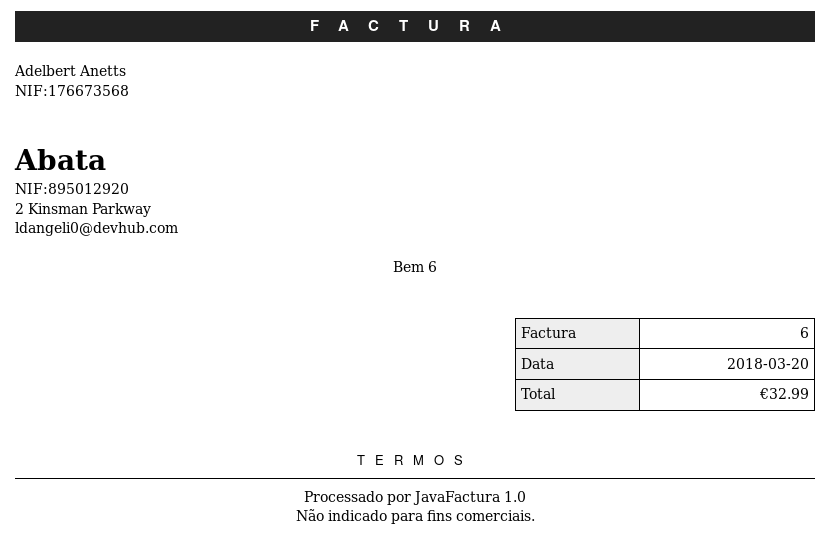
\includegraphics[scale=0.35]{imgs/factura.png}
\caption{Factura HTML.}
\label{img:factura}
\end{figure}

\subsection{Exportar e Importar informação em formato CSV}
\label{sec:csv}

Está disponível ao administrador da aplicação uma ferramenta de importação e
exportação de dados da aplicação. Este poderá fazer um \textit{dump} de todo o
conteúdo através de "Exportar CSV" para o ficheiro à sua escolha. Esta
funcionalidade percorre toda a estrutura de dados da aplicação e imprime todos
os objetos que ela contém para o ficheiro.

\begin{figure}[H]
\centering
\includegraphics[scale=0.35]{imgs/csv.png}
\caption{Ficheiro CSV.}
\label{img:csvfile}
\end{figure}

Poderá também, a qualquer momento carregar dados totais de um aplicação ou
pequena parcelas de dados, como por exemplo, apenas faturas de uma determinada
empresa, para a aplicação. O ficheiro importado é percorrido e para cada
objeto introduzido é feito o \textit{parse} do seus dados e depois é introduzido
na aplicação com recurso aos mesmo métodos usados no registo direto na
aplicação.

\begin{figure}[H]
\centering
\includegraphics[scale=0.35]{imgs/dashboardadmin.png}
\caption{Exportar/Importar CSV.}
\label{img:csv}
\end{figure}


\section{Conclusões}
\label{sec:conclusao}


Face ao problema apresentado e analisando criticamente a solução proposta concluímos
que cumprimos as tarefas, conseguindo atingir os objetivos definidos.
De facto, conseguimos implementar a aplicação que foi pedida.
Em particular pensamos as nossas estruturas de dados de forma a serem facilmente
adaptáveis a situações futuras, nomeadamente quando criamos a classe abstrata AtividadesEconomicas,
fizemo-lo com o intuito de facilitar a inserção de atividades económicas que conferissem direito
a dedução fiscal. Com efeito, para adicionar uma nova atividade, basta criar uma
nova subclasse, extensão da classe AtividadesEconomicas, que contenha
os dados necessários (código, designação, percentagem de dedução e limite) para a sua
implementação. Acresce que o mesmo se passa com o cálculo das deduções, visto que
este está associado ao setor de atividade económica. Com efeito, apesar da superclasse
definir o método calculaDeducao, que é herdado pelas subclasses que não o definem,
a maioria das subclasses de atividades económicas implementa o seu próprio método
calculaDeducao, fazendo-o da forma que considera mais adequada tendo em conta
diversos fatores, tais como a localização da empresa que presta o serviço ou o número
de elementos do agregado familiar.

Do mesmo modo, pensando em alterações futuras, implementamos a classe FamiliaNumerosa
com uma variável de classe que define o limite mínimo de dependentes, porquanto desta
forma podemos facilmente alterar a quantidade de dependentes que constituem uma família
numerosa para efeitos fiscais.
É ainda necessário aumentar a robustez da importação de CSV, que neste momento
tem muitas limitações, para se tornar mais útil a todos os utilizadores, de modo
a, que no futuro pudesse ser possível aos contribuintes fazer uso desta
ferramenta para maior conforto na introdução de dados.


Em suma, não obstante as potenciais melhorias que poderiam ser feitas no
programa, nomeadamente a introdução de diferentes taxas de IVA;
a discriminação dos bens ou serviços prestados, sobre os quais poderia incidir diferentes
taxas de IVA; a possibilidade do contribuinte individual ser capaz
de registar uma fatura emitida por uma empresa; a possibilidade de associar receitas
médicas a faturas de saúde com taxas de IVA superiores a 6\% e, finalmente, a implementação
do sorteio da \emph{Fatura da Sorte}, as quais não implementamos apenas por falta de tempo,
consideramos que o nosso projeto cumpre todos os requisitos pedidos.




\end{document}
